\documentclass[
    doctor,
    truefont, % just turn it on when using Windows
    %nofont, % remember to manally set the fonts
    pdflinks,
    %colorlinks,
    %compact,
    ]{setup/xjtuthesis}

\graphicspath{{figures/}}
\renewcommand{\vec}{}

\usepackage[section]{algorithm}
\usepackage{algorithmic}
\usepackage{hyperref}
\usepackage{tikz}
\usetikzlibrary{arrows}
\usepackage{pdfpages}
\usepackage{subfig}

\begin{document}

% 请修改 meta.tex 中的论文元信息
% 标题,中文
\ctitle{关于微分方程的辛方法和李群方法研究}

% 作者,中文
\cauthor{卢燚}

% 学科,中文,本科生不需要
\csubject{数学}

% 导师姓名,中文
\csupervisor{蒋耀林~~教授}

% 关键词,中文.用全角分号「;」分割
% 研究生的应首先从《汉语主题词表》中摘选
\ckeywords{波形松弛;辛方法;辛波形松弛方法;李群方法;微分方程}

% 提交日期,本科生不需要
%\cproddate{\the\year 年\the\month 月}
\cproddate{2016 年 12 月}

% 论文类型,中文,本科生不需要
% 从理论研究、应用基础、应用研究、研究报告、软件开发、设计报告、案例分析、调研报告、其它中选择
\ctype{应用基础}

% 论文标题,英文
\etitle{Research on Symplectic Method and Lie Group Method of Differential Equations}

% 作者姓名,英文
\eauthor{Yi Lu}

% 学科,英文,本科生不需要
\esubject{Mathematics}

% 导师姓名,英文
\esupervisor{Prof. Yao-Lin Jiang}

% 关键词,英文.用半角分号和一个半角空格「; 」分割
\ekeywords{Waveform relaxation; Symplectic method; Symplectic waveform relaxation method; Lie group method; Differential equations}

% 学科门类,英文
% 从Philosophy(哲学)、Economics(经济学)、Law(法学)、Education(教育学)、Arts(文学)、
%   Science(理学)、Engineering Science(工学)、Medicine(医学)、Management Science(管理学)中选择
\ecate{Science}

% 提交日期,英文,本科生不需要
% 应当和 cproddate 保持一致
%\eproddate{\monthname{\month}\ \the\year}
\eproddate{December\ 2016}

% 论文类型,英文,本科生不需要
% 从Theoretical Research(理论研究)、Application Fundamentals(应用基础)、Applied Research(应用研究)、
%   Research Report(研究报告)、Software Development(软件开发)、Design Report(设计报告)、
%   Case Study(案例分析)、Investigation Report(调研报告)、其它(Other)中选择
\etype{Application Fundamentals}

% 摘要,中文.段间空行
\cabstract{

高性能计算机以及集群的迅猛发展,使数值模拟成为了科学实验和工程实验领域里一个非常重要的工具,
一方面加速了产品产出的速度,另一方面给科学研究提供了极大便利.
随之而来的是不断涌现的新型数值计算方法和对更高精度更高效数值算法的需求.这些年来,数值计算领域的研究如雨后春笋般发展,日新月异.
数值计算的应用,尤其是微分方程数值模拟的应用更是遍及各个重要的工程领域乃至经济金融领域.随着工程和军
事上应用的蓬勃发展,对数值计算的精准性和时效性的要求日益迫切.在大规模集成电路模拟领域以及航空航天
领域,有一类相当重要的问题需要快速准确地求解,这使得针对快速高效数值计算方法的研究变得非常重要.

本文主要针对几类微分方程,研究讨论了辛(Symplectic)方法、辛波形松弛方法、李群方法和李点对称方法,
提出了几种便于实现并且计算速度快的计算方法.详细的研究内容和主要结论如下:

(一) 对于一类特殊类型的电报方程,应用辛方法进行计算.辛方法适用于哈密尔顿系统等具有特殊结构的
系统,然而电报方程本身不具有这样的结构.为了用辛方法计算,以获得更好的数值结果,我们首先使用了一个变换对其进行修正,然后再使用辛方法进行
求解,最后再用逆变换将数值结果变成原方程的数值结果.该算法的设计采用了和傅立叶变换方法类似的思想,即先变换再
求解再逆变换的思想.整体上讲,该方法利用了辛方法的优势,较好地计算了较长时间的电报方程的数值解.

(二) 对拓展 QZK 方程,利用李点对称方法,进行了一些方程的性质分析,并给出了方程的一些约化.李点对称
方法的思想是将李群作用到微分方程上,通过构造特定的变换,进而得到一些方程的性质甚至是精确解.我们根据 Ibragimov
新守恒律定理构造了拓展 QZK 方程的守恒律.同时,找到了一个最优系统的一维子代数,然后对最优子代数
系统进行了相似约化,将 $(2+1)$ 维拓展 QZK 方程约化为含有两个独立变量的线性偏微分方程.

(三) 基于哈密尔顿系统的辛方法,结合波形松弛方法,首次提出了辛波形松弛方法的概念,降低了原始问题隐式辛方法求解过程中的计算复杂程度,同时较辛方法相比缩短了计算时间.该方法利用了波形松弛方法解耦计算的优势,以及辛方法较好的长时间计算稳定性,将二种方法有机结合,达到一举两得的效果.该算法里波形松弛方法用来简化辛方法的求解
过程,辛方法用来指导波形松弛方法中分裂函数的选取,二者相得益彰.在此基础上,对于流形上的李群方程,利用
辛波形松弛方法的设计思想,提出了隐式 RK-MK 方法的波形松弛改造格式.李群方程属于流形上的微分方程,
原本在流形上的方程的解随着时间演变依然在流形上.但是使用传统的数值解法,数值解往往会脱离流形, RK-MK 方法就是使得数值结果依然落到流形上的一类方法,
该方法利用指数映射做到了这一点.然而,对于一些流形上保结构的问题,对 RK-MK 的
隐式格式需求依然会带来求解上的困难,故我们利用辛波形松弛方法的思想,设计出便于计算的格式,较好地解决了此问题.

在本文中,我们提出了一类电报方程的辛方法,哈密尔顿系统的辛波形松弛方法,以及该方法在流形上的一个
改造,并用李群方法来约化偏微分方程.在数值算例上显式出的较好的效果,约化的方程形式得到的化简,都说明了该
算法的有效性.最后,对工作进行了总结并对进一步研究进行了展望.

}

% 摘要,英文.段间空行
\eabstract{

At present, the rapid advancement of high performance computers as well as workstations has pushed numerical
simulation to a highly demanded position both in numerical analysis for science research and in numerical simulation
for industrial production, which reduces the cycle of science research and production. What it brings is numerous
approaches of numerical methods, the refreshing demands of high precision and efficient numerical algorithms as well as
numerous studies in this area. Scientific computation, especially computation for differential equations has been widely applied
in many areas and even in economical areas. As the applications in industrial and
military areas increased, the demands for high precision and real time numerical methods are urgent. Tremendous problems need to be solved
in large scale integrated circuits and space science fields, which emphasizes the importance of fast and efficient computing methods.

In this dissertation, our study focuses on symplectic method, symplectic waveform relaxation method, Lie group
method and Lie point symmetry method. Contributions and major conclusions are listed as follows:

(1) The symplectic method is applied to certain kind of telegraph equations. The symplectic method is often used to solve
Hamiltonian systems, which is not what normal telegraph equations can fit. Here, we take a pre-transform and then
solve it with the symplectic method, and afterwards drag the numerical solution back to the original telegraph equation
by an inverse transform. This idea resembles the idea of the Fourier transform method. They all solve equations in the
frequency domain and apply an inverse transform to bring the solution to the time domain. This method takes
advantage of the symplectic method, so it is expected to have long-term numerical results.

(2) For extended quantum Zakharov-Kuznetsov equations, we get some properties of this equation by the Lie point
symmetry method, and get a reduced equation. The Lie point symmetry method is a method that applies Lie group to differential
equations. With certain transforms, we can get some information of the equation as well as the solution. By the
theory of Ibragimov, a new conservation law is constructed for extended QZK equations. We find an optimal system of one dimensional
Lie subalgebras and reduce the equation with it so that the $(2+1)$ dimensional extended QZK equation is reduced
to a partial differential equation with two independent variables.

(3) Combining the symplectic method and the waveform relaxation method~(WR), we first propose a new method called
symplectic waveform relaxation for Hamiltonian systems, which makes it possible to compute a Hamiltonian system
``with waveform relaxation method''. The advantage is then a faster and easier method for Hamiltonian systems. It takes
advantage of both decoupling feature of the waveform relaxation method and long-term computation
feature of the symplectic method, which is also an organic combination for both. The waveform relaxation method is used to
simplify the symplectic method while the symplectic method is used to instruct how to choose splitting function of the waveform
relaxation method. After that, for Lie group equations on manifolds, based on
the idea of the symplectic waveform relaxation method, we come up with a new method of modifying the RK-MK method
for Lie group equations. Lie group equations are equations that depict flows on manifolds, whose solution lies on manifold.
Classical numerical methods cannot guarantee that the solution lies on the manifold, which is far from expectation.
The RK-MK method is then such a remedy, which uses exponential mapping to drag the solution back to
the manifold. However, some RK-MK schemes cannot ensure another requirement of structure preserving,
which leads to the need of implicit RK-MK. We propose a method to overcome the difficulty of solving with an implicit RK-MK method.

In conclusion, in this dissertation, we use the symplectic method to solve telegraph equations, we use the Lie point symmetry method
to reduce the extended QZK equation and propose a simple method for implicit numerical schemes by waveform relaxation for
Hamiltonian systems as well as for Lie group equations. Numerical experiments show the efficiency of
our numerical methods. The results also show that the reduced equation is easier than the original problems. At last, we give a conclusion
and an outlook.

}


\xjtuchead \xjtuehead \xjtucinfopage \xjtueinfopage \xjtutoc \xjtutoe \clearpage

% 主要符号表,可以没有
\begin{denotation}
    %\iffalse
        \item[$I$]                       单位矩阵
        \item[$\mathbb{R}$]              实数域
        \item[$\mathbb{R}^n$]           $n$~维实欧氏空间
        \item[$\mathbb{C}$]              复数域
        \item[$\mathbb{C}^n$]          $n$~维复欧氏空间
        \item[$\bar{A}$]					$A$~的共轭
        \item[$\wedge$]					楔积
        \item[$a^T$]          矩阵~$a$~的转置
        \item[$\mathcal{G}$]              $\mathcal{G}$~为李群
        \item[$\mathfrak{g}$]              $\mathfrak{g}$~为李代数
        \item[$\mbox{expm}(A)$]                矩阵~$A$~的矩阵指数
        \item[$\mbox{Ad}$]           矩阵的伴随表示
        \item[$\mbox{ad}$]          矩阵伴随表示的导数
        \item[$D$]			$D$~为全导数符号
        \item[$\equiv$]                  恒等号
        \item[$| \cdot |$]               绝对值
        \item[$\| \cdot \|$]             赋范线性空间中元素的范数


    %\fi
\end{denotation}

\xjtucontent

% 绪论
\chapter{绪论}
\echapter{Preface}

\section{研究背景和现状}
\esection{Research Background and State of the Art}

随着计算机软硬件的迅猛发展,计算机形态的日新月异,机器人科学和量子计算机的出现与
蓬勃发展,对高效高性能算法的研究变得越来越重要.性能好的便于求解的算法在工业生产中
起到了决定性的核心作用.算法的计算速度快,实现简单,性能稳定和可并行性已经成为许多领域里
的基本需求,拥有这些算法也就意味着拥有了国家的核心竞争力.在数学领域里,为工程应用中提供
这些高效高性能的算法,其现实意义和重要性是十分明显的.在工程应用中,我们关注这样一类特殊的问题,此类
问题对应具有守恒律的系统,也就对计算效果有特殊的要求.然而,方程的守恒律在通常的数值计算格式
中往往无法直接体现.对于一个本身具有守恒性质的微分方程,只有合理地设计数值格式,才能达到
高效稳定快速这些要求.

本论文对与方程守恒性质相关的一些高性能算法(包括具有守恒性质
或者近似有守恒性质微分方程的辛方法,辛波形松弛方法),李群方法以及微分方程的李点对称方法展开研究,通过改进与创新,获得稳定的易于实现的数值
方法,和微分方程的一些守恒性质.所涉及的方向包括电路模拟,哈密尔顿系统的计算,流形上
的数值计算,和偏微分方程的约化和解析解.

\subsection{电报方程}
\esubsection{Telegraph Equations}

传输线主要用来描述传输无线电频率的交变电流,反映的是当电流频率高到一定程度时的波的性质.
传输线广泛应用在信号传输,产生脉冲和信号过滤等领域.常见的传输线主要有平行线、同轴电缆、
带状线、微带线、波导管、介质波导和光纤,等等.电报方程,也称为传输线方程或电报员方程,
来源于Maxwell方程组,是描述传输线中电流电压属性的一类方程.更具体地讲,电报方程来源于这样的问题,
导体是无限个二端口元件连接而成,每一个元件都是很小的传输线元件.

现有的关于电报方程的求解方法通常分为两大类,第一类是求精确解,第二类是求数值解.精确解只对部分
方程有效,其他部分我们还需要用数值模拟来解决.求数值解的方法,从思想上可以分为两种,第一种是
用解析的方法,将解的波形迭代起来求解,第二种则是离散方程之后的数值计算.解析方法通过迭代波形,
使得结果逐渐逼近真解.常见的解析方法有 Exp-函数方法~\cite{naher2011exp}, Adomian 分解
方法~(ADM)~\cite{adomian1988areview,sheikholeslami2012analytical}, 变分迭代方
法~(VIM)~\cite{wu2013variational} 和同伦摄动方法~(HPM)~\cite{sheikholeslami2012homotopy}. 电报
方程的离散方法常见的有微分二次方法~(DQM)~\cite{jiwari2012numerical}, 交替迭代隐式
方法~(ADI) \cite{cui2013convergence}, 和 WENO 方法 \cite{borges2008improved,shen2014improvement}.
电报方程的系统能量随时间而指数衰减,不具有能量守恒律.经过研究,我们找到了这样一个变换 \cite{polyanin2001handbook}, 能够使电报方程变为
一个守恒的系统,而这种守恒性刚好能让我们利用辛方法进行求解.这样做的好处是能够有效地
求解更长的时间区间,同时能够获得更容易实现的数值格式.

\subsection{拓展 QZK 方程}
\esubsection{Extended QZK Equations}

拓展 quantum Zakharov-Kuznetsov~(QZK) 方程描述了等离子体里的物理现象.对于拓展 QZK 方程的
研究追溯到几年前, Zakharov 和 Kuznetsov \cite{abdou2011quant} 构造了描述由冷离子和热电子构成的
磁等离子体的非线性离子波 (IAWs) 的方程.量子等离子体及其它们的性质获得了越来越多的从理论
物理和实验物理角度的注意,主要由于它们在德布罗伊波长超过德拜波长接近费米波长时的带电载体特性 \cite{abdou2011quant,ahmed2013kinks,bhrawy2013soli,biswas20091soli,biswas2013soli,bluman2010appli,elganaini2011tra,godleswski2004the,guner2015bright,ibragimov2006inte}. 在均匀磁场里的弱非线性离子波的性质由量子 Zakharov-Kuznetsov 方程来刻画.这些年来,许多
研究者的关注越来越多,在不同的量子等离子体模型中研究了磁场的影响 \cite{ibragimov2007anew,iwasaki1990cylin,johnpilai2011sym,khan2008linear,krishnan2010sol,leveque1992num,linares2009well,linares2011local,morris2013soli,moslem2007soli,mothibi2015con,moussa2001simi,munro2014con,munro2000sta,mushtaq2005non,olver2000app,peng2008exact,sabry2009non}.

(2+1) 维 Zakharov-Kuznetsov (ZK) 方程的主要研究手段有正弦余弦方法,拓展双曲正切方法,
同伦分析方法 \cite{linares2009well}, 简化的 Hirota 方法 \cite{biswas2013soli,bluman2010appli}
和映射方法 \cite{morris2013soli}, 等等.带有非线性扩散项和时间相关系数的 (2+1) 维广义
Zakharov-Kuznetsov (gZK) 方程由孤立波拟设方法所研究 \cite{sabry2009non}. (3+1) 维 QZK
方程可以通过辅助方程方法 \cite{ahmed2013kinks} 和拓展 F 展开 (EFE) 方法得到 \cite{munro2000sta}.
在 \cite{ahmed2013kinks} 中作者使用了约化摄动方法正式地得到了拓展 quantum Zakharov-Kuznetsov (extended QZK) 方程
,该方程由广义拓展方法 \cite{guner2015bright}, Jacobi 椭圆正弦和余弦函数 \cite{biswas20091soli}
所研究.李点对称方法和极简方程方法也可以用来研究 Zakharov-Kuznetsov 方程 \cite{leveque1992num}.
此外,对于一类广义 (2+1) 维 Zakharov-Kuznetsov 方程也有类似的工作 \cite{moslem2007soli}.

\subsection{哈密尔顿系统}
\esubsection{Hamiltonian Systems}

在数学上, 哈密尔顿系统是由数学家 Hamilton 构造出来,用来描述物理系统的发展型方程.该系统
的表示方法,巧妙地引入动量的概念,将一个二阶问题转化为维数加倍的一阶问题.该表示
的优点是能够在无法求得该系统的解析解的情况下,阐明一些动力系统的性态.在工程应用中,包括
动力学、分子动力学、流体力学、量子力学、图像处理、天体力学和核工程等领域中的问题,都可以表示成
相应的哈密尔顿系统的形式 \cite{arieh2009afirst}.

对于哈密尔顿系统,有一类比较成熟的,适于计算较长时间区间的方法,即辛方法 \cite{feng2010symplectic}. 辛方法是求解
较长时间区间的哈密尔顿系统的行之有效的方法.用辛方法求解哈密尔顿系统给予人们新的启迪,指引着人们去寻找好的优美的方法.辛方法起源于
de Vogelaere (1956), Ruth (1983)和 冯康 (1985) 的工作 \cite{hairer2006geometric}, 其基本
思想是避开盲目对精度的要求,巧妙地利用哈密尔顿系统的辛结构,将保持该结构作为目标,构造
数值格式.近些年的理论和数值算例都验证了该方法的优越性,系统的数值能量能够保持在系统的
真实值附近波动.

数十年来,辛方法迅速发展起来,方法得到了不断地发扬光大 \cite{calvo1994numerical,leimkuhler2004simulating,hong2006multi,yang2009extended,monovasilis2013exponentially,xin2016birkhoffian,michalas2016numerical,liao2016multi}. 该方法数值结果证实了辛数值积分格式比非辛格式的优越性.因此辛方法在处理多体问题和
其他哈密尔顿系统问题上,有着较好的应用.常用的辛方法有辛欧拉方法,辛 Runge-Kutta 方法,
辛 Runge-Kutta-Nystr{\"o}m 方法 \cite{kalogiratou2014fourth,kalogiratou2015}, 辛 ERKN
方法 \cite{wang2014ahigh}, 哈密尔顿 BVM \cite{brugnano2014multi}, 等等.此外,
关于哈密尔顿系统的研究还有两步波形松弛方法 \cite{hassanzadeh2014two}, 针对非自治
哈密尔顿系统的方法 \cite{hong2000numerical,zhang2010anote}, 随机哈密尔顿方程的
方法 \cite{burrage2014structure,ma2015sto,fan2015using}, 多辛方法 \cite{wang2013multi} 和
最有控制系统的研究 \cite{li2015asym}, 等等.这些方法都直接或间接地利用了辛方法的特性,构造
出了较好的数值格式.我们还知道,辛 Runge-Kutta 方法均为隐式方法 \cite{sanz1988runge}, 即
没有显式的保辛的 Runge-Kutta 法.

\section{主要方法}
\esection{Main Methods}
在本小节,我们对本文中所用到的基本方法做出总结与简单介绍,这些方法包括辛方法,李群方法和波形松弛方法.

\subsection{辛方法}
\esubsection{The Symplectic Method}

辛方法是求解哈密尔顿系统的一类特殊的数值方法,该方法结合哈密尔顿系统的辛结构而提出,在计算过程中有着优秀的特性.

辛方法的定义是基于哈密尔顿系统的特性提出的.为了在数值计算上得到很好的效果,将辛格式定义为在
每个数值时间点上保持 $q$ 与 $p$ 的外微分二形式 $dq_{n+1}\wedge dp_{n+1}=dq_n\wedge dp_n$, 这里含有下指标的 $q$ 和 $p$
分别是在不同离散时间点上的广义位移和广义动量.为了使验证变得容易,有一个与之等价的易于进行验证
操作的定义,即对于一个单步的数值方法 $z_{n+1}=\Phi_h(z_n)$, 保持 $(\nabla\Phi_h)^TJ^{-1}(\nabla\Phi_h)=J^{-1}$.

辛格式的数值格式有很多,最简单的是隐式中点法,辛欧拉法, St\"{o}rmer-Verlet 方法,辛 Runge-Kutta 方法等等.
构造辛格式的方法也有很多,辛 Runge-Kutta 方法就是其中一种,还有基于生成函数的方法,多级单步格式等等.
并且基于保辛格式和保结构的数值方法的研究一直在不断发展.

关于辛方法的理论研究主要有辛 Runge-Kutta 方法的阶数分析,包括根树理论和 B 级数理论;保辛和保能量
的研究及其相互之间的关系研究;反相误差分析理论;哈密尔顿摄动理论;高震荡方程的辛方法;多步法理论;
数值格式的长时间性态理论等等.

\subsection{李群方法}
\esubsection{The Lie Group Method}

李群 \cite{wanner1983fun} 是包含群结构的微分流形.作为群,李群有两个代数运算,乘法和逆.同时作为
微分流形我们要求李群的两个代数作用是光滑映射.李群对应的李代数是李群在单位元处的切空间,李代数
作为一个线性空间,其上包含一个双线性映射,称为李括号,满足反对称交换律和 Jacobi 恒等式.

指数映射是连接李群和李代数的一个纽带,其定义为 $\mathrm{exp}: \mathfrak{g}\to \mathcal{G}$,
式中 $\mathfrak{g}=T\mathcal{G}$ 为 $\mathcal{G}$ 的切空间.这里我们要求有如下关系成立 $\mathrm{exp}(x)\mathrm{exp}(y)=\mathrm{exp}(xy)$.
矩阵李群是李群的一个特例,其群元素均为矩阵,对应的指数映射即为矩阵的指数函数
\begin{equation*}
	\mbox{expm}(A)=\sum_{j=0}^{\infty}\frac{A^j}{j!},
\end{equation*}}
由于其形式和指数函数的定义相同,这也是指数映射得名的原因.

本文中的李群方法是指使用李群作为工具的一系列方法的统称.所涉及的方法有流形上的李群方法和李点对称方法.

\subsubsection*{\textbf{流形上的李群方法}}

本文中我们研究的李群方程是指在流形上的矩阵方程
\begin{equation*}
	Y'=A(t,Y)Y,\quad t\geq 0,\quad Y(0)=Y_0,
\end{equation*}
式中 $Y_0\in G $, $A:\mathbb{R}^+\times G\to \mathfrak{g}$, 这里的 $Y$ 和 $A(t,Y)$ 都是时间相关的 $N\times N$ 的矩阵.

对于流形上的李群方程,我们知道其解的流随着时间依然保持在流形上.
通常来说,我们的数值计算都是在一个空间上进行的,常用的空间是平直的线性欧氏空间.
然而,有些方程具有特殊的意义,这些问题的解存在在一个流形上.可是,在全空间上数值计算的
误差存在会导致计算结果并不在该流形上.为了解决这一类问题,有一类流形上的李群算法被
设计出来,这些算法能够很好地保证数值解落在流形上. Runge-Kutta Munthe-Kaas(RK-MK) 算法就是这样一类方法.李群
方法起初是由 Crouch 和 Grossman \cite{crouch1993numerical} 提出来的,即所谓
的 Crouch-Grossman 方法,该方法得到了一系列地推广
\cite{faleinsen2001multi,zaletkin2010numerical,bulychev2001numerical,buono2003numerical,billo1992numerical}.
后来,在 1996 到 1999 年, Munthe-Kaas  等人提出了该方法的一个改进方法
\cite{mk1996lie,mk1997numerical,mk1998runge,mk1999high}, 即 MK-RK 方法,以及后面的一些推广 \cite{ostermann2010exponential,owren2000the,bruls2012lie,munthe2013onpost,garcla2011onalg}.
Crouch-Grossman 方法和 MK-RK 方法都用到了李群的指数映射,联结了李群这个流形和
李代数之间的关系,并且都利用了 Runge-Kutta 方法这种数值结构,使得阶数可以适当地提高,
而且常规意义下的李群方法均为显式方法,计算较为简便.

\subsubsection*{\textbf{李点对称方法}}

李点对称方法 \cite{olver2000app} 是基于单参数李群,将李群作用在微分方程上的一类方法.起初,该方法根据
李的三个定理,发现可以把常微分方程从高阶化成较低阶,或者求出一些特解.后来逐渐演变为对偏微分方程的约减,
从较高阶化为较低阶,或者从多元化为单元等.该方法是一种求解微分方程特解
或者约化微分方程的方法.其思想是将微分方程放到 Jet 空间中研究,该空间的自变量是原方程的自变量,因
变量和因变量的各阶导数或偏导数.将李群作用到该空间,我们通过某种设计变换的形式,可以程式化地得到
单参数李群,据此经过一系列计算,我们得到一些关于方程的性质或者方程解的性质.

本文中,我们基于 \cite{sjoberg2007dou} 进一步研究拓展 QZK 方程.守恒律在研究微分
方程中扮演了重要角色,因为守恒律往往对应着物理中的守恒律,比如质量守恒、能量守恒、
动量守恒、角动量守恒、电荷守恒或其他运动的约束 \cite{mushtaq2005non,song2013top,song2013dom}.
守恒律可以用来研究非线性偏微分方程解的存在唯一性和解的稳定性 \cite{wang2014soli}, 此外
也有关于数值解的研究 \cite{wazwaz2005exact,wazwaz2008the}. 因此,我们对拓展 QZK 方程研究了
偏微分方程的守恒性质,我们证明了 (2+1) 维拓展 QZK 方程是严格自共轭的,并且构造了其守恒律.
接着,我们给出了一维子代数最优系统.通过相应的相似不变量的相似变换, (2+1) 维拓展 QZK 方程
变为线性的偏微分方程.说明了李点对称方法对于拓展 QZK 方程是有效的,该结果对研究该方程
起到了积极的指导作用.

\subsection{波形松弛方法}
\esubsection{The WR Method}

波形松弛方法来源于对大规模集成电路系统的研究 \cite{lelarasmee1982waveform}. 电路中,我们知道,
有许多电路定理,和等效电路定理,可以将大规模电路转化成若干个等效电路.基于这个思想,才有了波形松弛方法
的雏形,分裂电路系统,迭代求解的过程.我们认为
波形松弛方法主要分为两个部分,选取分裂函数对系统分裂和对分裂后的系统迭代直至收敛
 \cite{jiang2009wr,burrage1995parallel,jacob1985waveform}. 首先,我们需要使用分裂函数
 将规模大的系统划分为较小规模的子系统,这些分裂之后的子系统之间可以是解耦的,因此可以
 并行求解.接下来是迭代,迭代的过程先分别求解子系统,再在系统之间交换信息,进行下一次迭代,
直到收敛.由此可见,波形松弛方法的显著特性是问题解耦和潜在的可并行性.波形松弛方法给我们
指出了一种不同的求解微分方程的迭代方式.它不是简简单单的通过求解离散过后的代数方程组的
松弛方法,而是通过对方程分裂而构造出来的一种函数迭代方法,是``波形''的迭代.波形松弛方法的
一个优点是能够把耦合的系统,通过分裂,在迭代过程中化为非耦合的系统,即解耦,对于一些问题
来讲,这为算法的并行计算提供了条件.同时,我们注意到,在我们计算的过程中,波形松弛方法能够
将一些只能隐式格式求解的问题,化为显式或者半隐式的格式即可求解的问题.

简而言之,波形松弛方法 \cite{jiang2009wr} 作为一个数学工具,思想起源于大规模集成电路的
求解方法.当系统的规模大到一定程度的时候,使用现有的计算资源求解该问题就变得困难,我们
可以通过分裂成更易于求解的小型系统来做.为了达到这个目标,我们选取分裂函数 $F(z,y)$ 使
得 $F(z,z)=f(z)$, 然后将方程中的 $f(z)$ 替换为 $F(z,y)$. 接下来为每一个子
系统选择一个合适的初始迭代,我们将 $F(z,y)$ 中的 $y$ 作为已知函数, $z$ 作为未知函数,这样
每次迭代的计算量就降低了.然而这样的一步计算不会得到系统的真实解,这是由于初值的选取和格式
的设计引起的.这要求我们要通过迭代来保证收敛到方程的真解.通常我们将其
记作 $\dot{z}^{k+1}=F(z^{k+1},z^{k})$, 式中 $k=0,1,\cdots$ 是迭代次数.

\section{论文的主要内容和组织结构}
\esection{Main Results and Organizations of the Dissertation}

本文主要涉及了三部分内容,研究了一类电报方程的辛方法,辛波形松弛方法,流形上改进的李群方法
和李点对称对偏微分方程的约化,主要研究内容和创新点如下:

(一) 在第~2~章,我们提出了一种新的求解带有齐次边界条件的电报方程的方法.该方法有效地利用了一个将非哈密尔顿系统化为哈密尔顿系统的变换,结合了辛方法的特性,得到了较好的效果.本章中,我们讨论了该算法的阶条件,~CFL 条件,长时间性质和局限性.在空间离散上我们取了二阶的离散格式,得到了 $O(\Delta x^2+ \Delta
t^k)$ 的误差界. 该方法的一个优点是利用了辛方法长时间求解的好的性质.另外, 我们的解可以看作一个很优美的哈密尔顿系统乘以一个函数的结果.我们方法的基本思想是先变换,再求解,再逆变换,和傅立叶变换的思想比较类似.数值结果展示了阶条件,算法的有效性和长时间性质.该方法不局限于使用文中提及的辛格式,其他合适的辛格式也可以使用进来.非齐次的问题,需要增加两个分量来求解,该部分在文中注解部分有所提及.

(二) 在第~3~章, 我们将复合变分准则应用到了 (2+1) 维拓展 QZK 方程.应用这些李点对称,我们证明了 (2+1) 维拓展 QZK 方程是自共轭的,并且构造了其守恒律.接着,我们给出了一维子代数最优系统.通过相应的相似不变量的相似变换, (2+1) 维拓展 QZK 方程约化为线性的偏微分方程.

(三) 在第~4~章,我们提出了求解哈密尔顿系统的辛波形松弛方法.该方法指明了针对该系统应该如何选择分裂函数的问题.我们使用窗口加速技术来加速该方法.我们给出了系统哈密尔顿量在迭代下收敛到守恒的量的性质,并在数值结果中验证了这一点.在此基础上,我们对李群方法做出了详细的介绍,分析了其优点和不足,并对隐式的 RK-MK 方法提出了一种改进方法,即用波形松弛方法进行修正.该方法能够缓解隐式 RK-MK 方法的复杂性计算问题,把隐式的计算化为较为简单的显式或者半隐式问题,同时利用窗口计算进行加速.我们还给出了算法的基本流程,通过数值结果说明了该方法的有效性.

在本文的最后,我们总结概括了本文的创新点,并对进一步的研究工作进行了展望.


% 以同样方法添加更多章节
\chapter{一类电报方程的辛方法研究}
\echapter{Study on Symplectic Method for Telegraph Equations}

本章介绍一类含有齐次初边值条件电报方程的辛方法,该方法的思想是利用一个特殊的变换,把不具有守恒性的电报方程,变为具有守恒性质的 Klein-Gordon 方程进行求解.对于变换后的守恒结构,我们结合辛方法进行求解.

传输线主要用来传输无线电频率的交变电流,反映了当电流频率高到一定程度时的波的性质.传输线广泛应用在信号传输,产生脉冲和信号过滤等领域.常见的传输线主要有平行线、同轴电缆、
带状线、微带线、波导管、介质波导和光纤,等等.电报方程,也称为传输线方程或电报员方程,来源于Maxwell方程组,是描述传输线里电流电压属性的一类方程.更具体地讲,电报方程来源于这样的问题,导体由无限个二端口元件连接而成,每一个元件都是很小的传输线元件.一般的传输线方程可以由图~\ref{fig:tele1} 中的等效模型,其关系可根据基尔霍夫电压和电流定律导出~\cite{ludwig2000rf}.

现有的关于求解电报方程的方法通常分为两大类,第一类是求精确解,第二类是求数值解.精确解只对一小部分方程有效,其他问题还需要用数值模拟来解决.求数值解的方法,从思想上可以分为两种,第一种是用解析的方法,将解的波形迭代起来求解,第二种则是离散方程之后的数值计算,即离散求解.解析方法通过迭代波形,使得结果逐渐逼近真解.常见的解析方法有 Exp-函数方法~\cite{naher2011exp}, Adomian 分解方法~(ADM)~\cite{adomian1988areview,sheikholeslami2012analytical}, 变分迭代方法~(VIM)~\cite{wu2013variational} 和同伦摄动方法~(HPM)~\cite{sheikholeslami2012homotopy}. 电报方程的离散方法常见的有微分二次方法~(DQM)~\cite{jiwari2012numerical}, 交替迭代隐式方法~(ADI) \cite{cui2013convergence}, 和 WENO 方法 \cite{borges2008improved,shen2014improvement}.

这里简要介绍各种解析方法的思想. Exp-函数方法是利用行波变换将偏微分方程转换为常微分方程,然后再将常微分方程的解用指数函数展成分式形式,过程中产生了一些待定常数,最后求解待定常数. Adomian 分解方法由 George Adomian 提出,该方法将算子的线性部分和非线性部分分裂开来,再设计迭代格式,是一种逼近真解的解析方法.变分迭代方法是一种迭代方法,主要有三个步骤,构造修正泛函,构造 Lagrange 乘子,确定初始迭代,其中第二步的构造 Lagrange 乘子是最重要的也是最困难的.同伦摄动方法和 Adomian 分解方法开始的步骤类似,将算子的线性部分和非线性部分分裂开来,然后再利用摄动方法,构造一个同伦,摄动的极限就是方程的真解.

常用的离散方法的基本思想如下.微分二次方法是把方程的每一项,包括函数值,及其各阶偏导数值,对于一组特殊的基进行展开,最后确定展开的系数,其衍生的方法有多项式微分二次方法等等.交替迭代隐式方法作为一种隐式差分数值格式,在高维问题的计算中有着较为好的效果,主要擅长计算热传导和扩散类方程.其思想是将一个有限差分格式沿着不同的空间方向分裂成两步,再进行计算.其优点是无条件稳定且时间空间二阶,也有更高阶的格式可以构造. WENO 方法是基于 ENO 方法提出来的,擅长于求解双曲型问题,比如交通流问题,波动类方程,等等.该方法是一种加权求值方法,通过特殊的构造权值,对 ENO 方法进行了改进,该方法对于分片光滑问题有着较好的效果.

本章所研究的是这样一类电报方程
\begin{equation}\label{eq:tele}
\left\lbrace
\begin{aligned}
&\frac{\partial ^2 w(x,t)}{\partial t^2}+k\frac{\partial w(x,t)}{\partial t}=a^2 \frac{\partial ^2 w(x,t)}{\partial x^2} + b w(x,t),\\
&\begin{aligned}
w(x,0)&=g_1(x),&0 \le x \le 1,\\
w_t(x,0)&=g_2(x),&0 \le x \le 1,\\
w(0,t)&=0,&0 \le t \le T,\\
w(1,t)&=0,&0 \le t \le T,
\end{aligned}
\end{aligned}
\right.
\end{equation}
式中 $k > 0$, $a>0$ 和 $b < 0$ 是常数. $g_1(x)$ 和 $g_2(x)$ 是光滑函数, 满足相容性条件 $g_1(0)=0$. $w(x,t) \in \mathbb{R}$ 为所求函数. 此方程对应于如下的一类传输线方程,方程的等效电路图如图~\ref{fig:tele1}. 图中,要求 $a^2 = \frac{1}{L_1C_1}, k= (\frac{R_2^{-1}}{C_1}+\frac{R_1}{L_1}), b =-\frac{R_1R_2^{-1}}{L_1C_1}$.
\begin{figure}[h]
    \centering
    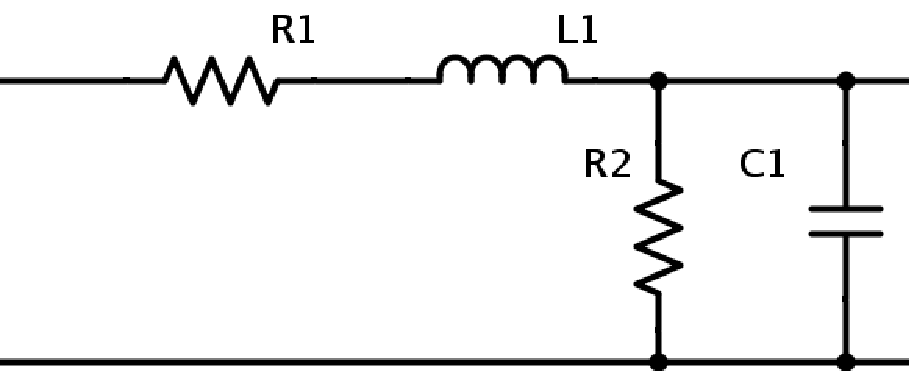
\includegraphics[width=0.5\textwidth]{02/Fig1.pdf}
    \caption{传输线方程的等效电路图}
    \label{fig:tele1}
\end{figure}

在本章中,我们针对具有齐次边界条件的电报方程 \eqref{eq:tele} 进行求解.该求解方法适用于一维和高维问题.本章的基本框架如下.首先在 \ref{sec:02symplectic} 中介绍辛方法.接下来,在 \ref{sec:02telegraph} 中逐步展开介绍我们的方法及其相关理论,数值结果将在 \ref{sec:02numerical} 中给出.最后一部分 \ref{sec:02conclusion} 是小结.

\section{辛的基本概念}\label{sec:02symplectic}
\esection{Introduction to the Symplectic Method}
辛方法 \cite{feng2010symplectic} 是求解较长时间区间的哈密尔顿系统的行之有效的方法.用辛方法求解哈密尔顿系统的做法给予人们新的启迪,指引着人们去寻找好的优美的方法.辛方法起源于 de Vogelaere (1956), Ruth (1983)和 冯康 (1985) 的工作 \cite{hairer2006geometric}, 其基本思想是避开盲目对精度的苛求,巧妙地利用哈密尔顿系统的辛结构,改为保持该结构作为目标,构造数值格式.理论和数值算例都验证了该方法的优越性,系统的数值能量能够保持在系统的真实值附近波动.数十年来,辛方法迅速发展起来,并且得到了不断地发扬光大 \cite{calvo1994numerical,leimkuhler2004simulating,hong2006multi,yang2009extended,monovasilis2013exponentially,xin2016birkhoffian,michalas2016numerical,liao2016multi}. 该方法数值算例证实了辛数值积分格式相比非辛格式的优越性.因此,在处理多体问题和其他哈密尔顿系统问题上,有着较好的应用.

哈密尔顿系统是由数学家 Hamilton 构造出来,用来描述物理系统的发展型方程.该表示的优点是能够在无法求得该系统的解析解的情况下,阐明一些动力系统的性态.在工程应用中, 包括动力学、分子动力学、流体力学、量子力学、图像处理、天体力学、核工程等领域在内的问题,都可以表示成如下的哈密尔顿系统的形式 \cite{arieh2009afirst}
\begin{equation}\label{eq:Hamiltonian}
\left\lbrace
\begin{aligned}
\frac{dq}{dt}&=\frac{\partial H}{\partial p},\\
\frac{dp}{dt}&=-\frac{\partial H}{\partial q},
\end{aligned}
\right.
\end{equation}
式中 $p \in \mathbb{R}^d$ 和 $q \in \mathbb{R}^d$ 为所求函数, $H=H(q,p)$ 是系统的哈密尔顿量.在实际应用中, $d$ 为该哈密尔顿系统的自由度, $q$ 与 $p$ 分别对应系统的广义位移和广义动量.在相空间 $\mathbb{R}^{2d}$ 上的标准辛形式是如下的二微分形式
\begin{equation*}
\omega = \sum_{i=1}^d d q_i \wedge d p_i.
\end{equation*}
保持哈密尔顿系统辛结构的数值方法称之为辛方法,在后面部分会给出准确的定义.常用的辛方法有隐式中点法,交错显式格式,基于 Pad\'{e} 逼近的方法, St\"{o}rmer-Verlet 格式,辛 Runge-Kutta 方法,等等.

在本小节,我们列出了几种具有代表性的辛格式.哈密尔顿系统具有一个守恒的哈密尔顿量 $H(q,p)$, 其中 $q$ 表示位移 $p$ 表示动量.


令 $\Phi_h : \mathbb{R}^{2d} \to \mathbb{R}^{2d}$ 表示时间步进的数值算法进行一步计算的函数, 其中 $d$ 为 $p$ 和 $q$ 的维数. $z_{n+1}=\Phi_h(z_n)$ 其中 $z_n$ 是在第 $n$ 步时间点上数值解.辛方法则是具有以下性质的一类方法.

\begin{definition}[辛方法~\cite{hairer2006geometric}]
\emph{一个单步的数值方法 $z_{n+1}=\Phi_h(z_n)$ 称为辛方法,如果该方法保持二形式
\begin{equation*}
dq_{n+1}\wedge dp_{n+1}=dq_n\wedge dp_n,
\end{equation*}
式中 $z_n=(q_n,p_n)^T,~n=1,2,\cdots$.}
\end{definition}

下面是辛方法的一个等价定义.

\begin{definition}[辛方法~\cite{hairer2006geometric}]\label{def:symplectic}
\emph{一个单步的数值方法 $z_{n+1}=\Phi_h(z_n)$ 称之为辛方法,如果 $\Phi_h$ 的 Jacobian 矩阵满足
\begin{equation*}
(\nabla\Phi_h)^TJ^{-1}(\nabla\Phi_h)=J^{-1}.
\end{equation*}}
\end{definition}

\begin{remark}
{\rm 定义 \ref{def:symplectic} 使得我们能够更容易验证数值格式的辛性质.为了获得更多的,更高阶的辛方法,需要使用生成函数法,见 \cite{hairer2006geometric}.}
\end{remark}

接下来,在这里给出一些辛方法的例子.

\noindent \textbf{隐式中点法}
\begin{equation*}
\frac{z^{n+1}-z^n}{\tau}=J^{-1}H_z(\frac{z^{n+1}+z^n}{2}),
\end{equation*}
为二阶辛方法.

\noindent \textbf{辛欧拉法}
\begin{equation*}
\begin{aligned}
p_{n+1}&=p_n-hH_q(p_{n+1},q_n),\\
q_{n+1}&=q_n+hH_p(p_{n+1},q_n),
\end{aligned}
\quad \text{or} \quad
\begin{aligned}
p_{n+1}&=p_n-hH_q(p_n,q_{n+1}),\\
q_{n+1}&=q_n+hH_p(p_n,q_{n+1}),
\end{aligned}
\end{equation*}
均为一阶方法.

\noindent \textbf{St\"{o}rmer-Verlet 格式}
\begin{equation*}
\begin{aligned}
p_{n+1/2}&=p_n-\frac{h}{2}H_q(p_{n+1/2},q_n),\\
q_{n+1}&=q_n+\frac{h}{2}(H_p(p_{n+1/2},q_n)+H_p(p_{n+1/2},q_{n+1})),\\
p_{n+1}&=p_{n+1/2}-\frac{h}{2}H_q(p_{n+1/2},q_{n+1}),
\end{aligned}
\end{equation*}
和
\begin{equation*}
\begin{aligned}
q_{n+1/2}&=q_n+\frac{h}{2}H_q(p_n,q_{n+1/2}),\\
p_{n+1}&=p_n-\frac{h}{2}(H_p(p_n,q_{n+1/2})+H_p(p_{n+1},q_{n+1/2})),\\
q_{n+1}&=q_{n+1/2}+\frac{h}{2}H_q(p_{n+1},q_{n+1/2}),
\end{aligned}
\end{equation*}
均为二阶方法.

\noindent \textbf{辛 Runge-Kutta 方法}

对于 Runge-Kutta 方法,我们知道, $\nu$ 步的 Runge-Kutta 方法可以写成
\begin{equation*}
  \left\lbrace
    \begin{aligned}
      Y_{n+1}^{r}&=\eta(t_{n})+h\sum_{s=1}^{\nu}a_{rs}f(t_{n+1}^{s},Y_{n+1}^{s}),\quad r=1,\cdots, \nu, \\
      \eta(t_{n+1})&=\eta(t_{n})+h\sum_{s=1}^{\nu}b_{s}f(t_{n+1}^{s},Y_{n+1}^{s}).
    \end{aligned}
  \right.
\end{equation*}

其对应的 Butcher 表可以写成

\begin{center}
  \begin{tabular}{c|cccc}
    $c_1$&$a_{11}$&$a_{12}$&$\cdots$&$a_{1\nu}$\\
    $c_2$&$a_{21}$&$a_{22}$&$\cdots$&$a_{2\nu}$\\
    $\vdots$&$\vdots$&$\vdots$&$\ddots$&$\vdots$\\
    $c_{\nu}$&$a_{\nu 1}$&$a_{\nu 2}$&$\cdots$&$a_{\nu \nu}$\\
    \hline
         &$b_{1}$&$b_{2}$&$\cdots$&$b_{\nu}$
  \end{tabular}
\end{center}

\begin{theorem}{辛 Runge-Kutta 方法\cite{sanz1988runge}}
\emph{如果该 Runge-Kutta 的 Butcher 表满足
\begin{equation*}
  b_ia_{ij}+b_ja_{ji}=b_ib_j,\quad \textrm{对所有}\,\, i,j=1,2,\cdots,\nu,
\end{equation*}
则该 Runge-Kutta 方法是保辛的.}
\end{theorem}

对于辛 Runge-Kutta 方法,它的阶数和对应的 Runge-Kutta 方法的阶数相同,可以用根树理论和B级数理论来求得.

\noindent \textbf{由生成函数构造的辛方法}

根据生成函数的构造理论,能够得到一系列如下的辛格式 \cite{feng2003sym}.

$1$ 阶格式

\begin{equation*}
	p_i^{k+1}= p_i^{k}-hH_{q_i}(p^{k+1},q^{k}),
\end{equation*}
\begin{equation*}
	q_i^{k+1}= q_i^{k}+hH_{p_i}(p^{k+1},q^{k}),
\end{equation*}
式中 $i=1,\ldots,n$.

$2$ 阶格式

\begin{equation*}
	p_i^{k+1}= p_i^{k}-hH_{q_i}(p^{k+1},q^{k})-\frac{h^2}{2}\sum_{j=1}^n(H_{q_j}H_{p_j})_{q_i}(p^{k+1},q^{k}),
\end{equation*}
\begin{equation*}
	q_i^{k+1}= q_i^{k}+hH_{p_i}(p^{k+1},q^{k})+\frac{h^2}{2}\sum_{j=1}^n(H_{q_j}H_{p_j})_{p_i}(p^{k+1},q^{k}),
\end{equation*}
式中 $i=1,\ldots,n$.

$3$ 阶格式

\begin{equation*}
\begin{aligned}
	p_i^{k+1}= &p_i^{k}-hH_{q_i}(p^{k+1},q^{k})-\frac{h^2}{2}\sum_{j=1}^n(H_{q_j}H_{p_j})_{q_i}(p^{k+1},q^{k})\\
	&-\frac{h^3}{6}\sum_{i,j=1}^n(H_{p_lp_j}H_{q_l}H_{q_j}+H_{q_lq_j}H_{p_l}H_{p_j}+H_{p_lq_j}H_{q_l}H_{p_j})_{q_i}(p^{k+1},q^{k}),
\end{aligned}
\end{equation*}
\begin{equation*}
\begin{aligned}
	q_i^{k+1}= &q_i^{k}+hH_{p_i}(p^{k+1},q^{k})+\frac{h^2}{2}\sum_{j=1}^n(H_{q_j}H_{p_j})_{p_i}(p^{k+1},q^{k})\\
	&+\frac{h^3}{6}\sum_{i,j=1}^n(H_{p_lp_j}H_{q_l}H_{q_j}+H_{q_lq_j}H_{p_l}H_{p_j}+H_{p_lq_j}H_{q_l}H_{p_j})_{p_i}(p^{k+1},q^{k}),
\end{aligned}
\end{equation*}
式中 $i=1,\ldots,n$.

\noindent \textbf{可分系统的多级显式方法}

对于可分的哈密尔顿系统, $H(q,p)=V(q)+U(p)$, 该系统可以写成
\begin{equation*}
	\frac{d}{dt}\begin{bmatrix}
	q\\
	p
	\end{bmatrix}=\begin{bmatrix}
	g(p)\\
	f(q)
	\end{bmatrix},
\end{equation*}
有如下一系列的多级显式格式 \cite{qin2011struc}.

$1$阶精度$1$级辛格式
\begin{equation*}
	p^{k+1}=p^{k}+hc_1f(q^{k}),\quad q^{k+1}=q^{k}+hd_1g(p^{k+1}),
\end{equation*}
式中 $c_1=d_1=1$.

$2$阶精度$2$级辛格式
\begin{equation*}
	\left\lbrace \begin{aligned}
		&p_1=p^{k}+hc_1f(q^{k}),\quad q_1=q^{k}+hd_1g(p_1),\\
		&p^{k+1}=p_1+hc_2f(q_1),\quad q^{k+1}=q_1+hd_2g(p^{k+1}),
	\end{aligned}\right.
\end{equation*}
式中 $c_1=0,c_2=1,d_1=d_2=\frac{1}{2}$ 或$d_1=1,d_2=0,c_1=c_2=\frac{1}{2}$.

$3$阶精度$3$级辛格式
\begin{equation*}
	\left\lbrace \begin{aligned}
		&p_1=p^{k}+hc_1f(q^{k}),\quad q_1=q^{k}+hd_1g(p_1),\\
		&p_2=p_1+hc_2f(q_1),\quad q_2=q_1+hd_2g(p_2),\\
		&p^{k+1}=p_2+hc_3f(q_2),\quad q^{k+1}=q_2+hd_3g(p^{k+1}),
	\end{aligned}\right.
\end{equation*}
式中
\begin{equation*}
	c_1=\frac{7}{24},\quad c_2=\frac{3}{4},\quad c_3=-\frac{1}{24},
\end{equation*}
\begin{equation*}
	d_1=\frac{2}{3},\quad d_2=-\frac{2}{3},\quad d_3=1,
\end{equation*}
或
\begin{equation*}
	c_1=1,\quad c_2=-\frac{2}{3},\quad c_3=\frac{2}{3},
\end{equation*}
\begin{equation*}
	d_1=-\frac{1}{24},\quad d_2=\frac{3}{4},\quad d_3=\frac{7}{24}.
\end{equation*}

$4$阶精度$4$级辛格式
\begin{equation*}
	\left\lbrace \begin{aligned}
		&p_1=p^{k}+hc_1f(q^{k}),\quad q_1=q^{k}+hd_1g(p_1),\\
		&p_2=p_1+hc_2f(q_1),\quad q_2=q_1+hd_2g(p_2),\\
		&p_3=p_2+hc_2f(q_2),\quad q_3=q_2+hd_2g(p_3),\\
		&p^{k+1}=p_3+hc_3f(q_3),\quad q^{k+1}=q_3+hd_4g(p^{k+1}),
	\end{aligned}\right.
\end{equation*}
式中
\begin{equation*}
	c_1=0,\quad c_2=c_4=\frac{1}{2}(2+\alpha),\quad c_3=-\frac{1}{4}(1+2\alpha),
\end{equation*}
\begin{equation*}
	d_1=d_4=\frac{1}{6}(2+\alpha),\quad d_2=d_3=\frac{1}{6}(1-\alpha),
\end{equation*}
或
\begin{equation*}
	c_1=\frac{1}{6}(2+\alpha),\quad c_2=c_3=\frac{1}{6}(1-\alpha),\quad c_4=\frac{1}{2}(2+\alpha),
\end{equation*}
\begin{equation*}
	d_1=\frac{1}{3}(2+\alpha),\quad d_2=-\frac{1}{3}(1+2\alpha),\quad d_3=\frac{1}{2}(2+\alpha),\quad d_4=0,
\end{equation*}
这里 $\alpha = 2^{\frac{1}{3}}+2^{-\frac{1}{3}}$.

\noindent \textbf{多级隐式辛方法}

这里举几个多级隐式辛格式 \cite{qin2011struc}
\begin{equation*}
	\left\lbrace \begin{aligned}
		&z^{k+1}=2Y_1-z^k,\\
		&Y_1=z^k+\frac{1}{2}hSY_1,
	\end{aligned}\right.
\end{equation*}

\begin{equation*}
	\left\lbrace \begin{aligned}
		&z^{k+1}=2Y_2-(2Y_1-z^k),\\
		&Y_1=z^k+\frac{1}{4}hSY_1,\\
		&Y_2=2Y_1-z^k+\frac{1}{4}hSY_2,
	\end{aligned}\right.
\end{equation*}

\begin{equation*}
	\left\lbrace \begin{aligned}
		&z^{k+1}=2Y_3-(2Y_2-2Y_1+z^k),\\
		&Y_1=z^k+\frac{1}{2}ahSY_1,\\
		&Y_2=2Y_1-z^k+\frac{1}{2}ahSY_2,\\
		&Y_3=2Y_2-(2Y_1-z^k)+(\frac{1}{2}-a)hSY_3,
	\end{aligned}\right.
\end{equation*}

\begin{equation*}
	\left\lbrace \begin{aligned}
		&z^{k+1}=2Y_4-(2Y_3-2Y_2+2Y_1-z^k),\\
		&Y_1=z^k+\frac{1}{2}b_1hSY_1,\\
		&Y_2=2Y_1-z^k+\frac{1}{2}b_2hSY_2,\\
		&Y_3=2Y_2-(2Y_1-z^k)+\frac{1}{2}b_3hSY_3,\\
		&Y_4=2Y_3-(2Y_2-2Y_1+z^k)+\frac{1}{2}b_4hSY_4,
	\end{aligned}\right.
\end{equation*}
式中 $a=1.351207,~ b_1=-2,703094,~ b_2=-0.536527,~ b_3=1.860681$.

令
\begin{equation*}
	S=\begin{bmatrix}
		0&M_1\\
		I&0
	\end{bmatrix}\quad \text{或} \quad S=\begin{bmatrix}
		0&M_3\\
		M_3&0
	\end{bmatrix},
\end{equation*}
则上面的格式依次有精度 $o(\Delta t+\Delta x^2),~o(\Delta t+\Delta x^2),~o(\Delta t^3+\Delta x^2),~o(\Delta t^4+\Delta x^2)$.

若取
\begin{equation*}
	S=\begin{bmatrix}
		0&M_2\\
		I&0
	\end{bmatrix}\quad \text{或} \quad S=\begin{bmatrix}
		0&M_4\\
		M_4&0
	\end{bmatrix},
\end{equation*}
则上面的格式依次有精度 $o(\Delta t+\Delta x^4),~o(\Delta t^t+\Delta x^4),~o(\Delta t^3+\Delta x^4),~o(\Delta t^4+\Delta x^4)$.
这里
\begin{equation*}
	M_1=\frac{1}{\Delta x^2}\begin{bmatrix}
		-2&1&0&\cdots&\cdots&1\\
		1&-2&1&\cdots&\cdots&0\\
		&\ddots&\ddots&\ddots&&\\
		&&\ddots&\ddots&\ddots&\\
		0&0&\cdots&\cdots&-2&1\\
		1&0&\cdots&\cdots&1&-2
	\end{bmatrix},\quad M_3=\frac{1}{2\Delta x}\begin{bmatrix}
		0&1&0&\cdots&\cdots&-1\\
		-1&0&1&\cdots&\cdots&0\\
		&\ddots&\ddots&\ddots&&\\
		&&\ddots&\ddots&\ddots&\\
		0&0&\cdots&\cdots&0&1\\
		1&0&\cdots&\cdots&-1&0
	\end{bmatrix},
\end{equation*}
\begin{equation*}
	M_2=\frac{1}{12\Delta x^2}\begin{bmatrix}
-30 & 16 & -1 & 0 & 0 & \cdots & \cdots & 0 & -1 & 16 \\
16 & -30 & 16 & -1 & 0 & \cdots & \cdots & 0 & 0 & -1 \\
-1 & 16 & -30 & 16 & -1 & \cdots & \cdots & 0 & 0 & 0 \\
\ddots & \ddots & \ddots & \ddots &   &   &   &   &   &   \\
&\ddots & \ddots & \ddots & \ddots &   &   &   &   &\\
&&\ddots & \ddots & \ddots & \ddots &   &   &   &-1\\
&&&\ddots & \ddots & \ddots & \ddots &   &   &-1\\
-1 & 0 & 0 & \cdots & \cdots & \cdots & -1 & 16 & -30 & 16 \\
16 & -1 & 0 & \cdots & \cdots & \cdots & 0 & -1 & 16 & -30
\end{bmatrix},
\end{equation*}
\begin{equation*}
	M_4=\frac{1}{12\Delta x}\begin{bmatrix}
0 & 8 & -1 & 0 & 0 & \cdots & \cdots & \cdots & 1 & -8\\
-8 & 0 & 8 & -1 & 0 & \cdots & \cdots & \cdots & 0 & 1\\
1 & -8 & 0 & 8 & -1 & \cdots & \cdots & \cdots && \\
\ddots & \ddots & \ddots & \ddots &   &   &   &   && \\
&\ddots & \ddots & \ddots & \ddots &   &   &   &&\\
&&\ddots & \ddots & \ddots & \ddots &   &   && \\
-1 & 0 & 0 & \cdots & \cdots & \cdots & 1 & -8 & 0&8 \\
8&-1 & 0 & 0 & \cdots  & \cdots & \cdots & 1 & -8 & 0
\end{bmatrix}.
\end{equation*}

辛方法是一大类方法的总称,其延伸及其推广包括辛 Runge-Kutta 法 \cite{feng2010symplectic,burrage2014structure}, 辛 RKN 方法 \cite{monovasilis2013exponentially}, 辛 ERKN 方法 \cite{yang2009extended}, 等等.这些方法中一部分为隐式方法,另外,辛 Runge-Kutta 方法均为隐式方法 \cite{sanz1988runge}.

\section{电报方程的辛方法}\label{sec:02telegraph}
\esection{Symplectic Methods for Telegraph Equations}

电报方程的系统能量随时间而指数衰减.经过研究,我们发现了这样一个能够使电报方程 \eqref{eq:tele} 变为一个守恒的系统的变换,而得到的这种守恒性刚好能让方程利用辛方法进行求解.这样做带来的好处是能够有效地求解更长的时间区间,获得更容易实现的数值格式.我们将在 \ref{sec:02transform} 节中详细介绍这种变换.

方程 \eqref{eq:tele} 的差分格式通常可以从两个角度来入手.一种是全离散,也就是说,对空间和时间进行等间距的网格的划分 $x_0=0<x_1<\cdots<x_N=1,~t_0=0<t_1<\cdots<t_n=T$. 之后,能够得到全离散的结果
\begin{equation}\label{eq:fulld}
\frac{w_{i}^{j+1}-2w_{i}^{j}+w_{i}^{j-1}}{\Delta t^2}+k\frac{w_{i}^{j+1}-w_{i}^{j}}{\Delta t}=a^2
\frac{w_{i+1}^{j+1}-2w_{i}^{j+1}+w_{i-1}^{j+1}}{\Delta x^2} + b w_{i}^{j+1},
\end{equation}
式中, $1 \le i \le N-1$ 和 $1 \le j \le n-1$. 式 $w_{i}^{j}$ 分别是在空间和时间格点上的数值,即$w(x_i,t_j)=w_{i}^{j}$.
另外一种则是半离散.如果取等间距的空间网格划分 $x_0=0<x_1<\cdots<x_N=1$, 将得到一个常微分方程组 (ODEs),
\begin{equation*}
\frac{d^2 W_i}{d t^2}+k\frac{d W_i}{d t}=a^2 \frac{W_{i+1}-2W_{i}+W_{i-1}}{\Delta x^2} + b W_i,
\end{equation*}
式中, $1 \le i \le N-1$, 和 $W_i = W(x_i,t)$. 这里,我们采用了时间二阶离散.

令 $W=(W_1,W_2,\cdots,W_{N-1})^T$, 则有
\begin{equation}\label{eq:fd}
\frac{d^2 W}{d t^2}+k\frac{d W}{d t}= -\frac{a^2}{\Delta x^2}SW + b W,
\end{equation}
式中
\begin{equation}\label{eq:s}
S=\begin{pmatrix}
2&-1&&&\\
-1&2&1&&\\
&-1&2&\ddots&\\
&&\ddots&\ddots&-1\\
&&&1&2
\end{pmatrix}.
\end{equation}

为了获得稳定的数值格式,在用差分方法求解方程 \eqref{eq:fd} 的时候,在时间离散上通常采用隐式格式.注意到如果方程 \eqref{eq:tele} 的边界条件适当,则可以将方程 \eqref{eq:fd} 写成哈密尔顿系统的形式.在此条件下,对方程 \eqref{eq:tele} 做一个变换,利用这个变换把方程 \eqref{eq:fd} 中的阻尼项 $k\frac{d W}{d t}$ 去掉.该变换能把一个电报方程变换成 Klein-Gordon 方程,因此能够得到更加容易求解的哈密尔顿系统.

接下来,针对一维和高维两种情况来介绍我们的算法 \ref{alg:tele}. 算法基本分三个步骤,即做变换,离散求解哈密尔顿系统,做逆变换得到数值解.

\begin{algorithm}
\caption{电报方程求解基本算法}
\begin{algorithmic}[1]
\STATE 将电报方程 \eqref{eq:tele} 变换成相应的 Klein-Gordon 方程. 相应地改变初边值条件. \newline
\STATE 离散 Klein-Gordon 方程为哈密尔顿方程组. 使用辛方法求解该哈密尔顿系统,得到 Klein-Gordon 方程的数值解. \newline
\STATE 对该数值解作用逆变换,得到电报方程的数值解.
\end{algorithmic}
\label{alg:tele}
\end{algorithm}

\subsection{变换的选取}\label{sec:02transform}
\esubsection{The Transformation Applied to Telegraph Equations}
现在回忆一下电报方程 \eqref{eq:tele}, 针对电报方程 \eqref{eq:tele} 本身来看,
\begin{equation}\label{eq:telegraph}
\frac{\partial ^2 w}{\partial t^2}+k\frac{\partial w}{\partial t}=a^2 \frac{\partial ^2 w}{\partial x^2} + b w.
\end{equation}

令 $w=e^{\lambda kt}u$, 并将其带入方程 \eqref{eq:telegraph}, 得到变换
$w=e^{-\frac{1}{2}kt}u$, 其中 $\lambda = -\frac{1}{2}$. 参见 \cite{polyanin2001handbook}.

同时,容易得到该变换的逆变换 $u=e^{\frac{1}{2}kt}w$. 注意到该变换和逆变换均不会产生数值上的误差,也就是说,我们算法的误差只隐含在求解哈密尔顿系统那一步里.

\begin{lemma}[由电报方程到 Klein-Gordon 方程的变换 \cite{polyanin2001handbook}]\label{thm:trans}
\emph{令 $w=e^{-\frac{1}{2}kt}u$, 电报方程 \eqref{eq:telegraph} 将变换成为如下的 Klein-Gordon 方程
\begin{equation}\label{eq:kg}
\frac{\partial ^2 u}{\partial t^2}=a^2 \frac{\partial ^2 u}{\partial x^2} + (b+\frac{1}{4}k^2) u.
\end{equation}}
\end{lemma}

对于 $n$ 维情形
\begin{equation}\label{eq:tele2d}
\frac{\partial ^2 w}{\partial t^2}+k\frac{\partial w}{\partial t}=a^2 (\frac{\partial ^2 w}{\partial x_1^2} +\cdots+
\frac{\partial ^2 w}{\partial x_n^2}) + b w,
\end{equation}
我们也可以得到相应的变换.

\begin{theorem}[$n$ 维情形]\label{thm:trans2}
\emph{令 $w=e^{-\frac{1}{2}kt}u$, 电报方程 \eqref{eq:tele2d} 将被变换成如下形式的 Klein-Gordon 方程
\begin{equation}\label{eq:kg2d}
\frac{\partial ^2 u}{\partial t^2}=a^2 (\frac{\partial ^2 u}{\partial x_1^2} +\cdots+ \frac{\partial ^2 u}{\partial x_n^2}) + (b+\frac{1}{4}k^2) u.
\end{equation}}
\end{theorem}

{\textbf{证明}} 注意到 $w=e^{-\frac{1}{2}kt}u$, 并且 $w$ 是电报方程 \eqref{eq:tele2d} 的解. 先来求 $w$ 的各阶偏导数.
\begin{align*}
\frac{\partial w}{\partial t} &= -\frac{1}{2}ke^{-\frac{1}{2}kt}u + e^{-\frac{1}{2}kt}\frac{\partial u}{\partial t},\\
\frac{\partial ^2 w}{\partial t^2} &=\frac{k^2}{4}e^{-\frac{1}{2}kt}u-ke^{-\frac{1}{2}kt}\frac{\partial u}{\partial t}
+e^{-\frac{1}{2}kt}\frac{\partial^2 u}{\partial t^2},\\
\frac{\partial ^2 w}{\partial x_i^2} &=e^{-\frac{1}{2}kt}\frac{\partial ^2 u}{\partial x_i^2},\quad i=1,2,\cdots,n.
\end{align*}

然后将得到的各阶导数代入 \eqref{eq:tele2d}, 两边同时除以 $e^{-\frac{1}{2}kt}$. 这样就得到了方程 \eqref{eq:kg2d}.

证毕.

接下来,需要知道初值和边值条件在该变换下的形式.通过一个简单的计算,即可得到相应的新的初值和边值条件,
\begin{equation}\label{eq:kgfull}
\left\lbrace
\begin{aligned}
&\frac{\partial ^2 u(x,t)}{\partial t^2}=a^2 \frac{\partial ^2 u(x,t)}{\partial x^2} + (b+\frac{1}{4}k^2) u(x,t),\\
&\begin{aligned}
u(x,0)&=g_1(x),&0 \le x \le 1,\\
u_t(x,0)&=g_2(x)+\frac{1}{2}k g_1(x),&0 \le x \le 1,\\
u(0,t)&=0,&0 \le t \le T,\\
u(1,t)&=0,&0 \le t \le T,
\end{aligned}
\end{aligned}
\right.
\end{equation}
式中 $k > 0$, $a>0$ 和 $b < 0$ 是常数. $g_1(x)$ 和 $g_2(x)$ 是光滑函数, $u(x,t) \in \mathbb{R}$ 为所求函数.该变换对高维情形同样适用,在此给出一个二维的例子
\begin{equation*}
\left\lbrace
\begin{aligned}
&\frac{\partial ^2 u(x,y,t)}{\partial t^2}=a^2 (\frac{\partial ^2 u(x,y,t)}{\partial x^2}+ \frac{\partial ^2 u(x,y,t)}{\partial y^2})
+ (b+\frac{1}{4}k^2) u(x,y,t),\\
&\begin{aligned}
u(x,y,0)&=g_1(x,y),&(x,y)\in \Omega,\\
u_t(x,y,0)&=g_2(x,y)+\frac{1}{2}k g_1(x,y),&(x,y)\in \Omega,\\
u(0,t)&=0,&0 \le t \le T,~(x,y)\in \partial\Omega .
\end{aligned}
\end{aligned}
\right.
\end{equation*}

\subsection{哈密尔顿系统的辛方法}
\esubsection{The Symplectic Method for Hamiltonian Systems}
通过观察可以知道,半离散方程 \eqref{eq:kgfull} 得到的常微分方程组可以写成哈密尔顿系统,因此可以使用辛方法来进行求解.通过前面变换(引理 \ref{thm:trans})得到的 Klein-Gordon 方程再进行半离散,就会得到正则的哈密尔顿系统.这也是选择此变换的原因.

\subsubsection{Klein-Gordon 方程的离散}
\esubsubsection{Discretization of Klein-Gordon Equations}
选取等间距的空间格点来进行半离散.取 $0=x_0<x_1<\cdots<x_{N-1}<x_N=1$ 式中 $x_i=i\Delta x,~i = 1,2,\cdots,N$.

令 $u_i(t)=u(x_i,t)$, $U=(u_1,u_2,\cdots,u_{N-1})^T$, 并取 $\frac{\partial u_n}{\partial
x}=\frac{u_{n+1}-2u_n+u_{n-1}}{\Delta x^2}$, 半离散的结果对应着如下的二阶系统
\begin{equation}\label{eq:aftert}
\left\lbrace
\begin{aligned}
&\frac{d^2U}{dt^2}=(-a^2 S+(b+\frac{1}{4}k^2)I) U,\\
&\begin{aligned}
U(0)=&(g_1(x_1),g_1(x_2),\cdots,g_1(x_{N-1}))^T,\\
U_t(0)=&(g_2(x_1)+\frac{1}{2}kg_1(x_1),g_2(x_2)\\
    &+\frac{1}{2}kg_1(x_2),\cdots,g_2(x_{N-1})+\frac{1}{2}kg_1(x_{N-1}))^T,
\end{aligned}
\end{aligned}
\right.
\end{equation}
式中
$S$ 在 \eqref{eq:s} 中定义, $I$ 是单位矩阵.

令 $q(t)=U(t),~ p(t)=U_t(t)$, 可以把二阶 ODE 写成如下一阶 ODE
\begin{equation}\label{eq:ode}
\left\lbrace
\begin{aligned}
\frac{dq}{dt}&=p,\\
\frac{dp}{dt}&=-Mq,
\end{aligned}
\right.
\end{equation}
初值条件为
\begin{equation*}
\left\lbrace
\begin{aligned}
q(0)&=U(0),\\
p(0)&=U_t(0),
\end{aligned}
\right.
\end{equation*}
式中 $M=a^2 S-(b+\frac{1}{4}k^2)I$,
$U(0)=(g_1(x_1),g_1(x_2),\cdots,g_1(x_{N-1}))^T$,
$U_t(0)=(g_2(x_1)+\frac{1}{2}kg_1(x_1),g_2(x_2)+\frac{1}{2}kg_1(x_2),\cdots,g_2(x_{N-1})+\frac{1}{2}kg_1(x_{N-1}))^T$.

可以看到, 方程 \eqref{eq:ode} 符合该形式的哈密尔顿系统 \eqref{eq:Hamiltonian}, 式中
$H(q,p)=\frac{1}{2}p^Tp+\frac{1}{2}q^TMq$, 因此,自然而然地选择辛方法来求解方程 \eqref{eq:aftert}.

对于二维的情形,同样采取等距的空间网格划分,二阶偏导项 $\frac{\partial ^2 u}{\partial x^2} + \frac{\partial ^2
u}{\partial y^2}$ 仍然能够写成一个对称矩阵. 只需要把 $S$ 换成
\begin{equation*}
\begin{pmatrix}
A&-I&&\\
-I&A&\ddots&\\
&\ddots&\ddots&-I\\
&&-I&A
\end{pmatrix}_{(N-1)^2,(N-1)^2},
\end{equation*}
式中
\begin{equation*}
A=\begin{pmatrix}
4&-1&&\\
-1&4&\ddots&\\
&\ddots&\ddots&-1\\
&&-1&4
\end{pmatrix}_{(N-1),(N-1)}.
\end{equation*}

\subsubsection{CFL 条件和阶条件分析}
\esubsubsection{Analysis of the CFL Condition and Order Conditions}
在数学上, Courant-Friedrichs-Lewy~(CFL) 条件是一种保证数值格式收敛的必要条件,尤其是适用于双曲偏微分方程的有限差分格式. CFL 条件的提出源自于对时间相关方程的时间步进数值格式的研究.该条件表明,时间步长必须取得足够小,才能保证计算过程中结果误差不会大得离谱.该条件由 Richard Courant, Kurt Friedrichs 和 Hans Lewy 在1928年的一篇文章中首次提出\cite{courant1967onthe}.本小节将给出 CFL 条件的选取方法,并且得出算法的阶.

对于本算法,因为 Klein-Gordon 方程和波动方程有相似的类型,所以取波动方程的 CFL 条件作为 Klein-Gordon 方程的 CFL 条件
\begin{equation*}
a^2\frac{\Delta t^2}{\Delta x^2}\le 1.
\end{equation*}
类似地,对于 $n$ 维问题,要求满足
\begin{equation*}
a^2 \frac{\Delta t^2}{\Delta x_1^2}+\cdots+a^2 \frac{\Delta t^2}{\Delta x_n^2}\le 1.
\end{equation*}

接下来,考虑相应的数值格式的阶条件,能够得到如下结论.

\begin{theorem}[算法 \ref{alg:tele} 的阶]\label{thm:tele}
\emph{算法 \ref{alg:tele} 在空间上是 $2$ 阶的,时间上是 $k$ 阶的,这里 $k$ 为辛格式的阶数.}
\end{theorem}

{\textbf{证明}} 想要得到算法 \ref{alg:tele} 的阶数,要考虑空间和时间上的离散.在空间方向,误差来源于对 $\frac{\partial^2
u}{\partial x^2}$ 一项的离散.如果取
\begin{equation*}
\frac{\partial^2u}{\partial x^2}\approx \frac{u_{i+1}-2u_i+u_{i-1}}{\Delta x^2},
\end{equation*}
那么可以得到
\begin{equation*}
\ddot{u}=Mu+O(\Delta x^2),
\end{equation*}
式中 $M$ 在公式 \eqref{eq:ode}中定义.

在时间方向,误差阶数取决于辛方法的数值阶数.一个 $k$ 阶的时间步进格式能够获得如下的阶
\begin{equation*}
\ddot{u}=Mu+O(\Delta t^k).
\end{equation*}
综上有
\begin{equation*}
\ddot{u}=Mu+O(\Delta x^2+ \Delta t^k).
\end{equation*}

证毕.

类似地,可以得到 $n$ 维电报方程 \eqref{eq:kg2d} 的阶条件,取等间距的空间网格划分
$0=x_{i,0}<x_{i,1}<\cdots<x_{i,N-1}<x_{i,N}=1,~i=1,2,\cdots,n$ 其中
$x_{i,j}=j\Delta x,~j = 1,2,\cdots,N$, 和二阶的空间离散
\begin{equation*}
\frac{\partial^2u}{\partial x_i^2}\approx \frac{u_{i,j+1}-2u_{i,j}+u_{i,j-1}}{\Delta x_i^2}.
\end{equation*}

\begin{theorem}[$n$ 维情形,算法 \ref{alg:tele} 的阶数]
\emph{算法 \ref{alg:tele} 在空间上是 $2$ 阶,时间上是 $k$ 阶,其中 $k$ 是辛格式的阶数.}
\end{theorem}

{\textbf{证明}} 证明的方法和定理 \ref{thm:tele} 的证明方法类似.

证毕.

此处,可以知道,对于辛方法,如果时间步长取得稍微大一点,仍然可以保持辛结构.然而,这种自由是有约束的,即受 CFL 条件约束.通常地,虽然时间步长理论中可以取得稍微大一些,但是还要考虑算法本身的计算的收敛性.为了保证整体数值结果的阶,还要考虑空间阶数.因此可以看到, CFL 条件和阶条件是两个影响数值解的条件.

二阶的空间离散能够得到一个对称矩阵,这样能够得到性质更好的哈密尔顿系统.所以,我们可以不限定离散格式的选取,其他能够离散成对称矩阵的格式都可以应用到此算法里.对于双线性的系统动能,即当广义位移的导数是广义动量的线性关系时,可以知道,保辛和保能量是等价的,但是,其他情况,没有一种数值算法既保辛又保能量.选取对称的离散的一个原因是,这样的选取能够保证哈密尔顿量即为系统的能量,于是算法既能量守恒又保辛,保持了系统的优美性.然而,在我们的算法里,这种选取并不是必要的.

这样得到的系统可以认为是可分的哈密尔顿系统.也就是说,任何求解可分哈密尔顿系统的方法,均可以用来求解此问题.

\subsection{辛方法的进一步讨论}
\esubsection{Further Discussions on the Symplectic Method}
我们的算法的主要思路是将辛方法这种性质优良的方法应用到电报方程上.然而,并不能直接这样做.原因是电报方程的阻尼项决定了系统不具有守恒性质.通过观察发现,一个将电报方程变为 Klein-Gordon 方程的变换能够使之得以下手,变换之后得到的是易于用辛方法求解的问题.鉴于这种变换的容易操作性,并且变换不会带来误差,我们会得到比较优良的算法.而且,由于辛方法的保结构性质,可以计算相对长一点的时间区间.

我们的算法框架是通过变换,变换成一个易于求解的问题,和逆变换,将求得的结果变回原方程的解.可以知道,傅立叶变换是将方程从时间域变换到频率域的算法.我们的算法和傅立叶变换方法有异曲同工之妙,可以看成在求解过程种做了一个从时间域到某个域的变换.只是使用的变换是一个简单的版本,因为变换和逆变换都很容易操作.

该算法的提出,一方面在于给出电报方法的一个新的解法,另一方面在于强调先变换,再求解,再逆变换的思想,这也是我们算法的核心和主要贡献.类似的方法有傅立叶变换的时域与频域的变换,李群方法的无穷小变换等等.

电报方程属于双曲型方程,因此,通常需要更高阶的方法才能获得较长时间的解.然而,应用了辛方法,可以适当降低对阶数的要求.同时,我们的算法也可以根据需要,构造时间和空间层面相对高阶数的算法.

此外,可以观察到,如果选取了显式的辛格式,那么求解的过程也是显式的,这对于时间相关的偏微分方程来说是有很高稳定性要求才能用的.同时可以知道,基于生成函数 \cite{feng2010symplectic} 的辛方法就有一类方法可以满足显式格式,这为我们格式选取提供了便利.

但是,我们的方法也有一些局限性,其中之一来自于对方程的边界条件的制约.只有一部分问题能够使用我们的方法,另外的部分要用到非自治哈密尔顿系统的辛方法.基本思想就是对非自治哈密尔顿系统做个变换,增加两个分量,得到非自治哈密尔顿系统,再进行求解.

考虑如下的非自治系统
\begin{equation*}
	\frac{dq_i}{dt}=\frac{\partial H}{\partial p_i},
\end{equation*}
\begin{equation*}
	\frac{dp_i}{dt}=-\frac{\partial H}{\partial q_i},
\end{equation*}
式中 $i=1,2,\ldots,n$, 哈密尔顿函数显含 $t$, 即 $H=H(p_1,\ldots,p_n,q_1,\ldots,q_n,t)$. 选择新的参数 $\tau$ 作为新的独立变量,设 $q_{n+1}:=t$ 和 $p_{n+1}=h=-H$, 得到扩充相空间上的方程

\begin{equation*}
	\frac{dq_i}{d\tau}=\frac{\partial H}{\partial p_i},\quad \frac{dp_i}{d\tau}=-\frac{\partial H}{\partial q_i},\quad i=1,2,\ldots,n
\end{equation*}
\begin{equation*}
	\frac{dp_{n+1}}{d\tau} = -\frac{\partial H}{\partial q_{n+1}},
\end{equation*}
\begin{equation*}
	\frac{dq_{n+1}}{d\tau} =1.
\end{equation*}

写成矩阵的形式就是
\begin{equation*}
	\frac{dz}{dt}=J\nabla K(z),\quad J=J_{2n+2}=\begin{bmatrix}
	0&-J_{2n+1}\\
	J_{2n+1}&0
	\end{bmatrix},
\end{equation*}
式中
\begin{equation*}
	\begin{aligned}
		K(z)&=h+H(p_1,\ldots,p_n,q_1,\ldots,q_n,t)\\
		&=p_{n+1}+H(p_1,\ldots,p_n,q_1,\ldots,q_n,q_{n+1}),
	\end{aligned}
\end{equation*}
称为扩充的哈密尔顿函数.

对于非自治的问题,也可以先寻找类似的变换,再借用上面关于非自治系统的求解方法进行求解,这个变换通常是类似的,这里不再赘述.

该变换对于电报方程组来说,需要加一些其他限制.对于方程
\begin{equation*}
\frac{\partial ^2 w}{\partial t^2}+K\frac{\partial w}{\partial t}=M \frac{\partial ^2 w}{\partial x^2} + N w,
\end{equation*}
如果取
\begin{equation*}
w=e^{-\frac{1}{2}Kt}u,
\end{equation*}
则有
\begin{equation*}
\frac{\partial ^2 u}{\partial t^2}= e^{\frac{1}{2}Kt} M e^{-\frac{1}{2}Kt}\frac{\partial ^2 u}{\partial x^2} +
e^{\frac{1}{2}Kt}(N+\frac{1}{4}K^2)e^{-\frac{1}{2}Kt} u,
\end{equation*}
式中 $K,M,N$ 是矩阵. 所以,可以知道需要满足条件 $MK=KM$ 和 $NK=KN$ 才能使用该变换.

\section{数值实验}\label{sec:02numerical}
\esection{Numerical Experiments}

在本节我们对几个电报方程的例子分别利用不同辛方法来求解.其中两个例子是一维的方程,一个是二维的方程.通过数值结果,可以看到阶条件的结果.由于 $a^2$ 较小的时候,数值结果较为容易求解,因而例子中的 $a^2$ 取的相对不那么小,这样能够更好地展示算法的有效性.在例子结尾将对其给出分析.

\subsection{数值算例}
\esubsection{Examples}

\subsection*{算例 1}
在此例中,取方程 \eqref{eq:telegraph} 中的参数为 $k = 8\pi,~a = 2$ 和 $b
= -3\pi^2$.

此例的精确解是 $w(x,t) = e^{-\pi t}sin(\pi x)$. 初值和边值条件分别为
\begin{equation*}
\begin{aligned}
w(x,0)&=\sin(\pi x),\\
w_t(x,0)&=-\pi \sin(\pi x),
\end{aligned}
\end{equation*}
和
\begin{equation*}
\begin{aligned}
w(0,t)&=0,\\
w(1,t)&=0.
\end{aligned}
\end{equation*}

通过变换 $w = e^{-4\pi t}u$, 得到方程 \eqref{eq:kg}, 其中初值条件为
\begin{equation*}
\begin{aligned}
u(x,0)&=\sin(\pi x),\\
u_t(x,0)&=3\pi \sin(\pi x),
\end{aligned}
\end{equation*}
边值条件为
\begin{equation*}
\begin{aligned}
u(0,t)&=0,\\
u_t(1,t)&=0.
\end{aligned}
\end{equation*}

我们用了辛欧拉方法 (一阶),隐式中点法 (二阶) 和 St\"{o}rmer-Verlet 方法 (二阶).作为对比,采用隐式欧拉法来``直接''求解电报方程 \eqref{eq:telegraph}, 并记为``直接方法''.直接方法使用的是全离散格式.针对这个问题,隐式中点法在实际计算过程中是显式求解的,见 \cite{feng2010symplectic}. 我们来检验结果的阶和长时间性质.

\textbf{$\Delta x$ 的阶}

首先,为了得到 $\Delta x$ 的阶,固定一个较小的 $\Delta t$, 然后相应地变化 $\Delta x$. 结果在表 \ref{tab:dx1} 中给出. 这里取 $\Delta t=0.001$ 和 $T=2$,可以看到 St\"{o}rmer-Verlet 方法为二阶的.

\begin{table}[h]
  \centering
\caption{随 $\Delta x$ 的变化,不同方法的误差的无穷范数变化情况比较,其中 $\Delta t=0.001$, $T=2$}
\begin{tabularx}{\linewidth}{XXXXX}
 \toprule[1.5pt]
 $\Delta x$ &直接方法 & 辛欧拉 & 隐式中点 & St\"{o}rmer-Verlet\\
 \midrule[1pt]
 0.1 & 0.0026 & 0.0011 & 0.0025 & 0.0017\\
 0.05 & 0.0010 & 0.0013 & 0.0012 & 4.2103e-04\\
 0.025 & 6.8722e-04 & 0.0014 & 9.2472e-04 & 1.0098e-04\\
 0.0125 & 6.0390e-04 & 0.0015 & 8.4536e-04 & 2.1029e-05\\
 0.00625 & 5.8372e-04 & 0.0015 & 8.2554e-04 & 3.5435e-06\\
 \bottomrule[1.5pt]
\end{tabularx}
  \label{tab:dx1}
\end{table}

\textbf{$\Delta t$ 的阶}

其次,固定一个较小的 $\Delta x$, 相应地变化 $\Delta t$, 得到表 \ref{tab:dt1} 的结果. 此处的参数 $\Delta x$ 和 $\Delta t$ 取值时比较困难. 一方面 CFL 条件要求 $\Delta t$ 取得相对于 $\Delta x$ 小一些.另一方面,为了验证阶条件, $\Delta x$ 一定要比 $\Delta t$ 小才能看到 $\Delta t$ 的变化.

然后我们看一下理论结果里的阶 $O(\Delta x^2+ \Delta t^k)$. 如果 $k =
1$, 我们可以固定很小的 $\Delta x$, 通过变化 $\Delta t$ 来看阶数. 然而,当 $k \ge 2$, 这个阶数不是很容易得到检验. 取 $\Delta x = 0.01$, 结果在表 \ref{tab:dt1} 中给出,可以看到辛欧拉方法为一阶的, St\"{o}rmer-Verlet 方法为二阶的.

\begin{table}[h]
  \centering
\caption{随 $\Delta t$ 的变化,不同方法的误差的无穷范数变化情况比较,其中 $\Delta x=0.01$, $T=2$}
\begin{tabularx}{\linewidth}{XXXXX}
 \toprule[1.5pt]
 $\Delta t$ &直接方法 & 辛欧拉 & 隐式中点 & St\"{o}rmer-Verlet\\
 \midrule[1pt]
 0.01 & 0.0057 & - & 8.3585e-04 & - \\
 0.005 & 0.0029 & 0.0074 & 2.2122e-04 & 1.5288e-04 \\
 0.0025 & 0.0015 & 0.0037 & 6.7965e-05 & 3.0713e-05 \\
 0.00125 & 7.3818e-04 & 0.0018 & 2.9746e-05 & 8.5729e-06 \\
 0.000625 & 3.7797e-04 & 9.0788e-04 & 2.0234e-05 & 1.4851e-05 \\
 \bottomrule[1.5pt]
\end{tabularx}
  \label{tab:dt1}
\end{table}

\textbf{长时间性质}

最后, 固定 $\Delta x$ 和 $\Delta t$, 变化时间区间 $T$ 来检验长时间的性质,得到表 \ref{tab:t1} 中的结果. 这里,步长分别取为 $\Delta x = 0.05$ 和 $\Delta t = 0.001$, 可以看到所有方法长时间性质良好.

\begin{table}[h]
  \centering
\caption{随 $T$ 的变化,不同方法的误差的无穷范数变化情况比较,其中 $\Delta x=0.05$, $\Delta t=0.001$}
\begin{tabularx}{\linewidth}{XXXXX}
 \toprule[1.5pt]
 $T$ &直接方法 & 辛欧拉 & 隐式中点 & St\"{o}rmer-Verlet\\
 \midrule[1pt]
 1 & 0.0010 & 0.0013 & 4.3489e-04 & 1.7282e-04 \\
 10 & 0.0010 & 0.0013 & 4.3489e-04 & 4.2674e-04 \\
 100 & 0.0010 & 0.0013 & 4.3489e-04 & 4.2674e-04 \\
 1000 & 0.0010 & 0.0013 & 4.3489e-04 & 4.2674e-04 \\
 10000 & 0.0010 & 0.0013 & 4.3489e-04 & 4.2674e-04 \\
 \bottomrule[1.5pt]
\end{tabularx}
  \label{tab:t1}
\end{table}

表 \ref{tab:t1} 中的结果对于每种方法随时间变化很小, 主要是因为精确解在 $T$ 足够大的时候趋近于 $0$ 了. 所以在以后的结果中,数值已经被表示为 $0$, 这由 ``IEEE 二进制浮点数算术标准''所定义.

为了更好地呈现误差随时间变化的结果,我们画了在 $[0,5]$ 区间中的误差,见图 \ref{fig:err1}.

\begin{figure}[h]
    \centering
    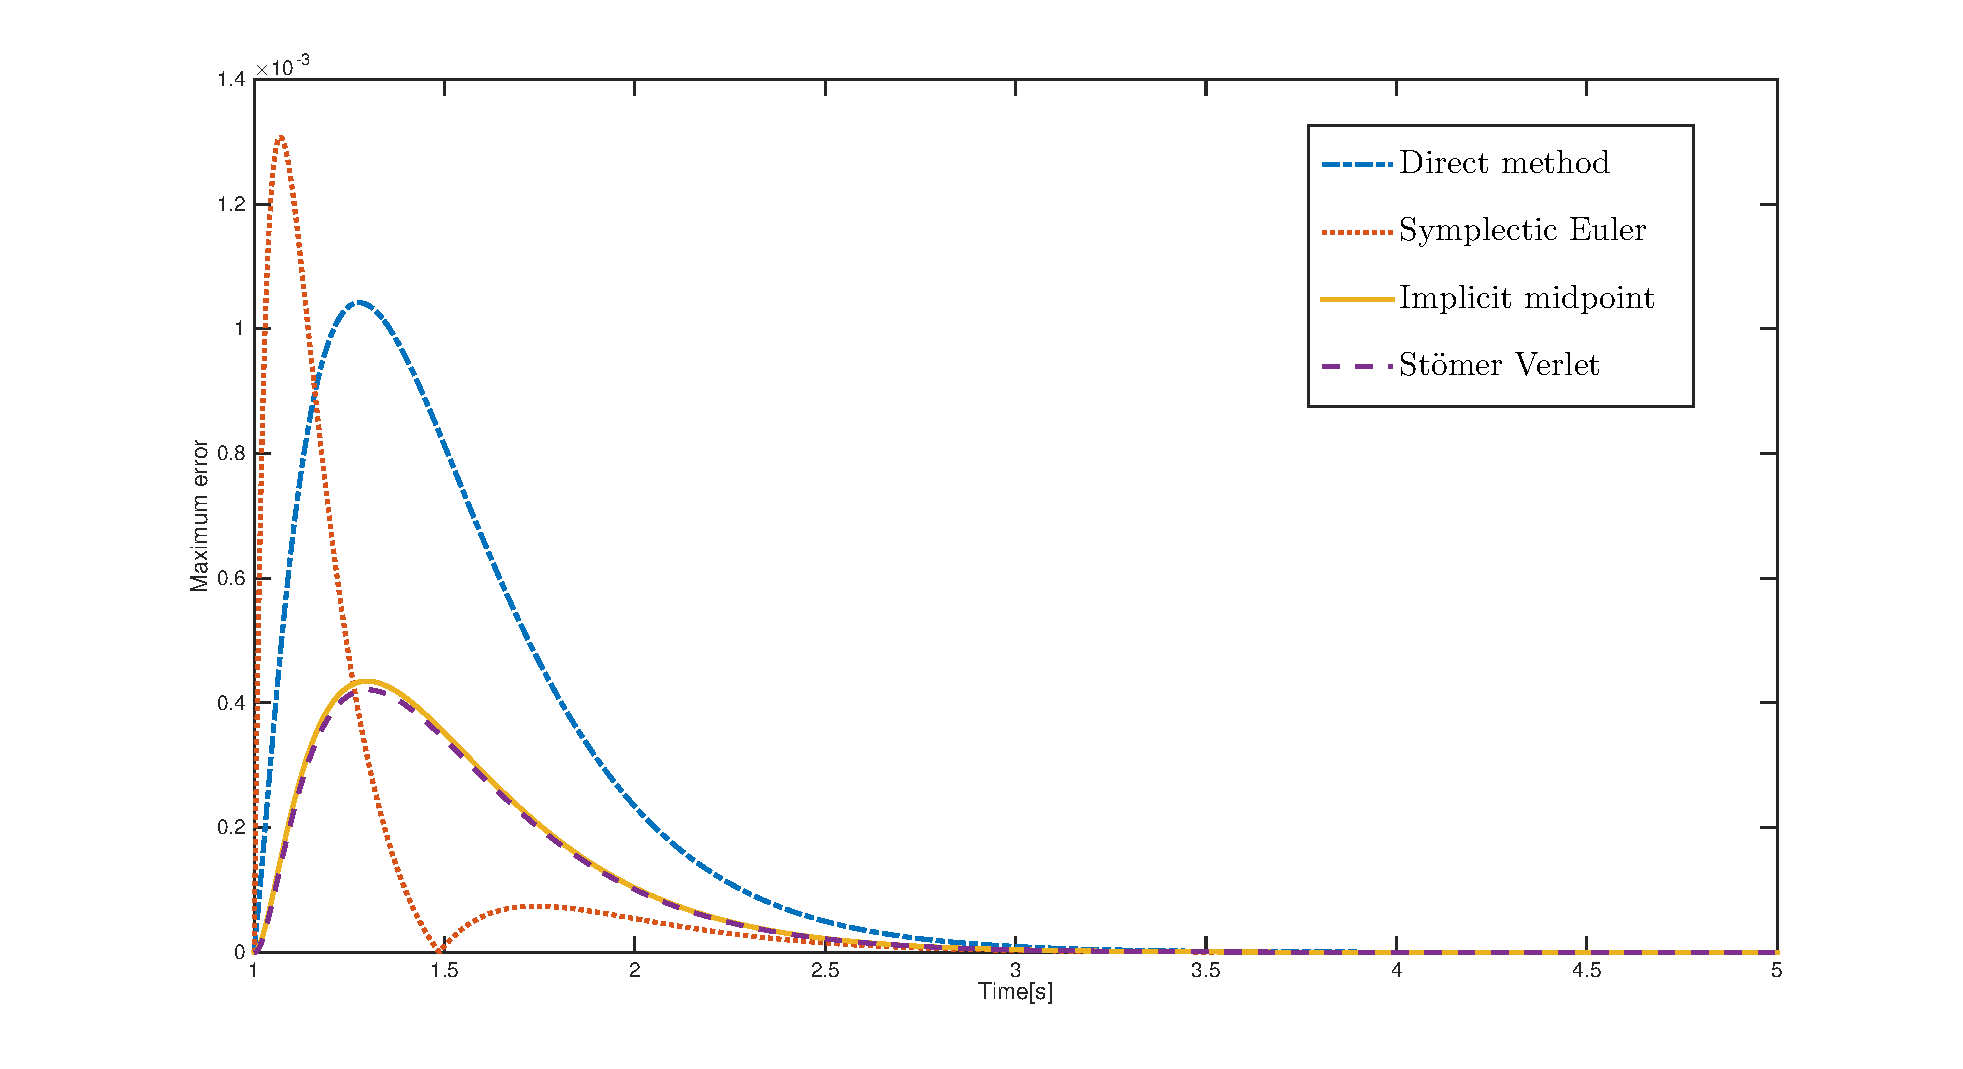
\includegraphics[width=0.8\textwidth]{02/Fig2.pdf}
    \caption{4种方法在 $[0,5]$ 区间的误差无穷范数的变化结果}
    \label{fig:err1}
\end{figure}


\subsection*{算例 2}
在此例中,取方程中的参数为 $a = 100, b
=-100\pi$ 和 $k =30\pi$. 并进行和算例 1 中同样的计算.
精确解为 $e^{-10\pi t}\sin(\pi t)$. 初值和边值条件分别为
\begin{equation*}
\begin{aligned}
w(x,0)&=\sin(\pi x),\\
w_t(x,0)&=-10 \pi \sin(\pi x),
\end{aligned}
\end{equation*}
和
\begin{equation*}
\begin{aligned}
w(0,t)&=0,\\
w(1,t)&=0.
\end{aligned}
\end{equation*}

通过变换 $w=e^{-15\pi t}u$, 得到方程 \eqref{eq:kg}, 其中初值条件为
\begin{equation*}
\begin{aligned}
u(x,0)&=\sin(\pi x),\\
u_t(x,0)&=5\pi \sin(\pi x),
\end{aligned}
\end{equation*}
边值条件为
\begin{equation*}
\begin{aligned}
u(0,t)&=0,\\
u_t(1,t)&=0.
\end{aligned}
\end{equation*}

数值结果如下.

\textbf{$\Delta x$ 的阶}

首先,为了检验 $\Delta x$ 的阶, 固定比较小的 $\Delta t$, 通过相应地变化 $\Delta x$ 来得到. 取 $\Delta t = 0.0001$, 和 $T
= 1$, 结果在表 \ref{tab:dx2} 中给出,可以看到隐式中点法和 St\"{o}rmer-Verlet 方法为二阶的.

\begin{table}[h]
  \centering
\caption{随 $\Delta x$ 的变化,不同方法的误差的无穷范数变化情况比较,其中 $\Delta t=0.0001$, $T=1$}
\begin{tabularx}{\linewidth}{XXXXX}
 \toprule[1.5pt]
$\Delta x$ &直接方法 & 辛欧拉 & 隐式中点 & St\"{o}rmer-Verlet\\
 \midrule[1pt]
 0.1 & 0.6487 & 0.0013 & 0.0013 & 0.0013\\
 0.05 & 0.6496 & 2.7325e-04 & 3.3279e-04 & 3.3271e-04\\
 0.025 & 0.6498 & 6.2785e-05 & 8.3249e-05 & 8.3174e-05\\
 0.0125 & 0.6499 & 8.6850e-05 & 2.0839e-05 & 2.0764e-05\\
 0.00625 & 0.6499 & 9.5203e-05 & 5.2348e-06 & 5.1600e-06\\
 \bottomrule[1.5pt]
\end{tabularx}
  \label{tab:dx2}
\end{table}

\textbf{$\Delta t$ 的阶}

其次,固定较小的 $\Delta x = 0.01$, 相应地变化 $\Delta t$, 得到表 \ref{tab:dt2} 的结果,可以看到直接方法为一阶的.

\begin{table}[h]
  \centering
\caption{随 $\Delta t$ 的变化,不同方法的误差的无穷范数变化情况比较,其中 $\Delta x=0.01$, $T=2$}
\begin{tabularx}{\linewidth}{XXXXX}
 \toprule[1.5pt]
 $\Delta t$ &直接方法 & 辛欧拉 & 隐式中点 & St\"{o}rmer-Verlet\\
 \midrule[1pt]
 0.001 & 0.6467 & 9.7975e-04 & 1.6714e-05 & 9.4887e-06 \\
 0.0005 & 0.6485 & 4.8457e-04 & 1.4153e-05 & 1.2295e-05 \\
 0.00025 & 0.6493 & 2.3809e-04 & 1.3524e-05 & 1.3057e-05 \\
 0.000125 & 0.6498 & 1.1523e-04 & 1.3368e-05 & 1.3251e-05 \\
 0.0000625 & 0.6500 & 5.4100e-05 & 1.3329e-05 & 1.3299e-05 \\
 \bottomrule[1.5pt]
\end{tabularx}
  \label{tab:dt2}
\end{table}

\textbf{长时间性质}

最后,固定 $\Delta x = 0.01$ 和 $\Delta t = 0.001$, 改变时间区间 $T$ 来查看长时间性质,得到表 \ref{tab:t2} 中的结果,可以看到所有方法长时间性质良好.

\begin{table}[h]
  \centering
\caption{随 $T$ 的变化,不同方法的误差的无穷范数变化情况比较,其中 $\Delta x=0.01$, $\Delta t=0.001$}
\begin{tabularx}{\linewidth}{XXXXX}
 \toprule[1.5pt]
 $T$ &直接方法 & 辛欧拉 & 隐式中点 & St\"{o}rmer-Verlet\\
 \midrule[1pt]
 1 & 0.6467 & 9.7975e-04 & 1.6714e-05 & 9.4887e-06 \\
 10 & 0.6467 & 9.7975e-04 & 1.6714e-05 & 9.4887e-06 \\
 100 & 0.6467 & 9.7975e-04 & 1.6714e-05 & 9.4887e-06 \\
 1000 & 0.6467 & 9.7975e-04 & 1.6714e-05 & 9.4887e-06 \\
 \bottomrule[1.5pt]
\end{tabularx}
  \label{tab:t2}
\end{table}

\subsection*{算例 3}
在此例中,我们求解二维的电报方程,
\begin{equation*}
\frac{\partial ^2 w}{\partial t^2}+8\pi \frac{\partial w}{\partial
t}=4 (\frac{\partial ^2 w}{\partial x^2} + \frac{\partial ^2
w}{\partial y^2}) -3\pi^2 w.
\end{equation*}
精确解为 $w(x,t) = e^{-\pi t}sin(\pi x)sin(\pi y)$. 初值和边值条件能够相应地得到,这里不再赘述.

\textbf{$\Delta x$ 的阶}

首先,固定 $\Delta t$, 相应地变化 $\Delta x$, 并取
$\Delta t = 0.0001$ 和 $T = 1$. 得到表 \ref{tab:dx3} 中的结果,可以看到隐式中点法和 St\"{o}rmer-Verlet 方法为二阶的.

\begin{table}[h!]
  \centering
\caption{随 $\Delta x$ 的变化,不同方法的误差的无穷范数变化情况比较,其中 $\Delta t=0.001$, $T=2$}
\begin{tabularx}{\linewidth}{XXXXX}
 \toprule[1.5pt]
 $\Delta x$ &直接方法 & 辛欧拉 & 隐式中点 & St\"{o}rmer-Verlet\\
 \midrule[1pt]
 0.1 & 0.8252 & 0.0018 & 0.0017 & 0.0017\\
 0.05 & 0.8301 & 5.0684e-04 & 4.2688e-04 & 4.2674e-04\\
 0.025 & 0.8314 & 2.0812e-04 & 1.0680e-04 & 1.0667e-04\\
 0.0125 & 0.8317 & 1.5813e-04 & 2.6763e-05 & 2.6625e-05\\
 \bottomrule[1.5pt]
\end{tabularx}
  \label{tab:dx3}
\end{table}

\textbf{$\Delta t$ 的阶}

其次,固定一个较小的 $\Delta x = 0.01$, 相应地变化 $\Delta t$, 得到了表 \ref{tab:dt3} 的结果,可以看到辛欧拉方法为一阶的.

\begin{table}[h]
  \centering
\caption{随 $\Delta t$ 的变化,不同方法的误差的无穷范数变化情况比较,其中 $\Delta x=0.01$, $T=1$}
\begin{tabularx}{\linewidth}{XXXXX}
 \toprule[1.5pt]
 $\Delta t$ &直接方法 & 辛欧拉 & 隐式中点 & St\"{o}rmer-Verlet\\
 \midrule[1pt]
 0.001 & 0.8317 & 0.0015 & 2.5175e-05 & 1.1497e-05 \\
 0.0005 & 0.8317 & 7.3588e-04 & 1.9097e-05 & 1.5646e-05 \\
 0.00025 & 0.8317 & 3.7202e-04 & 1.7581e-05 & 3.0713e-05 \\
 0.000125 & 0.8317 & 1.8992e-04 & 1.7203e-05 & 8.5729e-06 \\
 \bottomrule[1.5pt]
\end{tabularx}
  \label{tab:dt3}
\end{table}

\textbf{长时间性质}

最后,固定 $\Delta x = 0.1$ 和 $\Delta t = 0.001$, 通过变化求解区间长度 $T$ 来查看长时间性质,得到表 \ref{tab:t3} 的结果,可以看到所有方法长时间性质良好.

\begin{table}[h]
  \centering
\caption{随 $T$ 的变化,不同方法的误差的无穷范数变化情况比较,其中 $\Delta x=0.1$, $\Delta t=0.001$}
\begin{tabularx}{\linewidth}{XXXXX}
 \toprule[1.5pt]
 $T$ &直接方法 & 辛欧拉 & 隐式中点 & St\"{o}rmer-Verlet\\
 \midrule[1pt]
 1 & 0.8252 & 0.0026 & 0.0017 & 0.0017 \\
 10 & 0.8599 & 0.0026 & 0.0017 & 0.0017 \\
 100 & 0.8599 & 0.0026 & 0.0017 & 0.0017 \\
 1000 & 0.8599 & 0.0026 & 0.0017 & 0.0017 \\
 \bottomrule[1.5pt]
\end{tabularx}
  \label{tab:t3}
\end{table}

\subsection{结果分析}
\esubsection{Analysis of Results}

根据数值实验的结果,可以得到如下结论.首先,数值结果的全局误差由 CFL 条件和步长来制约.其次,由于全局误差界为 $O(\Delta x^2+ \Delta t^k)$, 能够在数值解上近似地看出阶条件.在这里,可以知道数值结果符合阶条件,和理论值相匹配.第三,长时间性质能够很好地保持.

此外,对于过长时间的计算是不必要的,因为该问题在一定长的时间后数值衰减得很小,超过机器误差的最小值,故不做过长计算.

\begin{remark}
{\rm 注意到,这里我们没有对哈密尔顿量的结果进行比较,因为变化之后,数值上比较大,哈密尔顿量的变化会很灵敏.此时,可能要求比较相对误差,然而该系统的哈密尔顿量保持在常值 $0$, 又使得我们无法使用相对误差作为衡量.因此需要一个更精妙的数值格式来保持,或者寻找一个新的评价标准来分析该方法的效果.然而,根据上述误差结果,我们有理由相信算法的有效性.}
\end{remark}

\section{小结}\label{sec:02conclusion}
\esection{Brief Summary}
在本章中,提出了一种新的求解带有齐次边界条件的电报方程的方法.该方法有效地利用了一个将非哈密尔顿系统化为哈密尔顿系统的变换,结合了辛方法的特性,得到了较好的效果.我们讨论了该算法的阶条件,~CFL 条件,长时间性质和局限性.在空间离散上取了二阶的离散格式,得到了 $O(\Delta x^2+ \Delta
t^k)$ 的误差界. 该方法的优势在于利用了辛方法长时间求解的好的性质.另外, 我们的解可以看作一个很优美的哈密尔顿系统乘以一个函数的结果.我们方法的基本思想是先变换,再求解,再逆变换,和傅立叶变换的思想比较类似.数值结果展示了阶条件,算法的有效性和长时间性质.该方法不局限于使用文中提及的辛格式,其他合适的辛格式也可以使用进来.非齐次的问题,需要增加两个分量来求解,该部分在文中注解部分有所提及.


\chapter{基于李群方法的拓展 QZK 方程研究}
\echapter{Study on Extended QZK Equations Based on the Lie Group Method}

%\section{拓展量子 Zakharov-Kuznetsov 方程简介}
%\esection{Introduction to extended quantum Zakharov-Kuznetsov equation}
2011年, Zakharov 和 Kuznetsov \cite{abdou2011quant} 构造了描述由冷离子和热电子构成的磁等离子体的非线性离子波 (IAWs) 的方程.量子等离子体及其它们的性质从此获得了越来越多的从理论物理和实验物理角度的注意,这是因为它们在德布罗伊波长超过德拜波长接近费米波长时的带电载体特性 \cite{abdou2011quant,ahmed2013kinks,bhrawy2013soli,biswas20091soli,biswas2013soli,bluman2010appli,elganaini2011tra,godleswski2004the,guner2015bright,ibragimov2006inte}. 在均匀磁场里的弱非线性离子波的性质由 quantum Zakharov-Kuznetsov (QZK) 方程来刻画.许多研究者在不同的量子等离子体模型中研究了磁场的影响 \cite{ibragimov2007anew,iwasaki1990cylin,johnpilai2011sym,khan2008linear,krishnan2010sol,leveque1992num,linares2009well,linares2011local,morris2013soli,moslem2007soli,mothibi2015con,moussa2001simi,munro2014con,munro2000sta,mushtaq2005non,olver2000app,peng2008exact,sabry2009non}.

(2+1) 维 Zakharov-Kuznetsov (ZK) 方程的主要研究手段有正弦余弦方法,拓展双曲正切方法,同伦分析方法 \cite{linares2009well}、 简化的 Hirota 方法 \cite{biswas2013soli,bluman2010appli} 和映射方法 \cite{morris2013soli}, 等等.带有非线性扩散项和时间相关系数的 (2+1) 维广义 Zakharov-Kuznetsov (GZK) 方程由孤立波拟设方法所研究 \cite{sabry2009non}. (3+1) 维 QZK 方程可以通过辅助方程方法 \cite{ahmed2013kinks} 和拓展 F 展开 (EFE) 方法得到 \cite{munro2000sta}. 在 \cite{ahmed2013kinks} 中作者使用了约化摄动方法正式地得到了拓展 quantum Zakharov-Kuznetsov (extended QZK) 方程,该方程由广义拓展方法 \cite{guner2015bright}、 Jacobi 椭圆正弦和余弦函数 \cite{biswas20091soli} 所研究.李点对称方法和极简方程方法也可以用来研究 Zakharov-Kuznetsov 方程 \cite{leveque1992num}.此外,对于一类广义 (2+1) 维 Zakharov-Kuznetsov 方程也有类似的工作 \cite{moslem2007soli}.

Wazwaz \cite{elganaini2011tra} 研究了一类新的拓展 (2+1) 维 QZK 方程, (3+1) 维 QZK 方程和 (3+1) 维拓展 QZK 方程.

其中,新的 (2+1) 维拓展 QZK 方程的形式如下:
\begin{equation}\label{eq:eqzk}
u_{t}+auu_{x}+b(u_{xxx}+u_{yyy})+c(u_{xyy}+u_{xxy})=0,
\end{equation}
式中 $a,~b$ 和 $c$ 为常实数, $u(x, y, t)$ 表示等离子体中静电场波的势能.它是空间变量 $x,~y$ 和暂态变量 $t$ 的函数.方程 \eqref{eq:eqzk} 中的第一项为暂态发展项,系数 $a$ 和非线性项的系数 $b$ 和 $c$ 是多维空间扩散系数.

针对上述方程,作者采用了极简形式的 Hirota 方法,得到了多孤子解和爆破解 \cite{biswas2013soli,bluman2010appli}. 李点对称方法也有应用到 \eqref{eq:eqzk} 方程中的相关研究 \cite{sjoberg2007dou}.

在本章中,我们将基于文献 \cite{wang2014soli} 进一步研究拓展 QZK 方程.守恒律在研究微分方程中扮演了重要角色,
在物理中有一些守恒律与之对应,比如质量守恒、能量守恒、动量守恒、角动量守恒、电荷守恒或其他运动的约束 \cite{mushtaq2005non,song2013top,song2013dom}. 守恒律可以用来研究非线性偏微分方程的存在唯一性和解的稳定性 \cite{wang2014soli}, 此外也有关于数值解的研究 \cite{wazwaz2005exact,wazwaz2008the}. 因此,也有必要研究偏微分方程的守恒性质.

本章的结构安排如下.首先,在 \ref{sec:05lie} 中介绍李点对称方法.其次,给出了利用李点对称方法得到的一些结果.在 \ref{sec:05con} 中,根据 Ibragimov 新守恒律定理构造了拓展 QZK 方程的守恒律.接下来,在 \ref{sec:05optimal} 中,找到了一个最优系统的一维子代数.然后在 \ref{sec:05reduction} 中,对最优子代数系统进行了相似约化,将 (2+1) 维拓展 QZK 方程约化为含有两个独立变量的线性偏微分方程.最后做了小结.

\section{李点对称方法}\label{sec:05lie}
\esection{The Lie Point Symmetry Method}
李点对称方法 \cite{peter2000sym,bluman2008symmetry} 基本思想是将李群作为变换群,将代数学中群作用到集合上的思想自然平移过来,其作用对象是微分方程,该作用达到将一个复杂的微分方程变换为较为简单的微分方程的目的.

在此过程中,需要寻找一个变换,寻找该变换是李点对称方法的核心问题之一.一个常用的方法是用李点对称,该方法程式化程度高,将复杂地寻找变换的过程变成了机械的符号计算过程.李点对称的思想是保持变换的每一阶导数和偏导数的形式,这样就能保证方程形式在变换之后和原来方程一致.

下面,首先介绍一些李群变换方法的相关知识.

\subsection{基本概念}
\esubsection{Basic Definitions}
这一章介绍李群的一般性质,下一章要针对矩阵李群进行讨论.
首先从李群的定义开始 \cite{kirillov2008anintro}, 逐步介绍一些李群的性质,以及后面要用到的李代数的相关内容.

\begin{definition}[实的李群]
	\emph{一个实的李群 $\mathcal{G}$ 是一个包含两个结构的集合: $\mathcal{G}$ 是一个群, $\mathcal{G}$ 是一个流形.这两个结构满足如下的条件:
	\begin{itemize}
		\item 群的乘积映射 $\mathcal{G}\times\mathcal{G}\to \mathcal{G}$ 是光滑映射,
		\item 逆映射 $\mathcal{G}\to \mathcal{G}$ 是光滑映射.
	\end{itemize}}
\end{definition}

\begin{definition}[复的李群]
	\emph{一个复的李群 $\mathcal{G}$ 是一个包含两个结构的集合: $\mathcal{G}$ 是一个群, $\mathcal{G}$ 是一个复解析流形.这两个结构满足如下的条件:
	\begin{itemize}
		\item 群的乘积映射 $\mathcal{G}\times\mathcal{G}\to \mathcal{G}$ 是解析映射,
		\item 逆映射 $\mathcal{G}\to \mathcal{G}$ 是解析映射.
	\end{itemize}}
\end{definition}

接下来举一些李群的例子
\begin{description}
	\item[(1)] $R^n~+$;
	\item[(2)] $S^1=\{z\in \mathbb{C}:|z|=1 \},~\times$;
	\item[(3)] $SU(2)=\{A \in GL(2,\mathbb{C})|A\bar{A}^T=1,det A = 1\},~\times$. 能够看出
	\begin{equation*}
		SU(2)=\left\lbrace\begin{pmatrix}
			\alpha&\beta\\
			-\bar{\beta}&\alpha
		\end{pmatrix}:\alpha,\beta\in\mathbb{C},|\alpha|^2+|\beta|^2 = 1
		 \right\rbrace.
	\end{equation*}
\end{description}

接着给出李子群的定义:
\begin{definition}[李子群]
	\emph{李群 $\mathcal{H}$ 是李群 $\mathcal{G}$ 是李子群,如果 $\mathcal{H}$ 是 $\mathcal{G}$ 的浸入子流形,并且是子群.}
\end{definition}

有了李子群的定义,就有了代数里面群的映射、同态、同构等代数工具来研究李群.

\begin{definition}[李群在流形上的作用]
	\emph{李群 $\mathcal{G}$ 在流形 $M$ 上的作用是对于任意 $g\in \mathcal{G}$ 的一个微分同胚映射 $\rho(g) \in \mathrm{Diff}~M$, 满足 $\rho(1) = id$ 和 $\rho(gh)=\rho(g)\rho(h)$ 使得
	\begin{equation*}
        \mathcal{G} \times M \to M : (g, m) \mapto \rho(g).m
	\end{equation*}
	是一个光滑映射,这里 $\mathrm{Diff}~M$ 为 $M$ 上的微分同胚群.}
\end{definition}

\begin{definition}[复李群在复流形上的全纯作用]
	\emph{复李群 $\mathcal{G}$ 在复流形 $M$ 上的全纯作用是对于任意 $g\in \mathcal{G}$ 的一个可逆全纯映射 $\rho(g) \in \mathrm{Diff}~M$, 满足 $\rho(1) = id$ 和 $\rho(gh)=\rho(g)\rho(h)$ 使得
	\begin{equation*}
        \mathcal{G} \times M \to M : (g, m) \mapto \rho(g).m
	\end{equation*}
	是一个全纯映射.}
\end{definition}

李群在流形上的作用是后面研究李群对偏微分方程的变换的基础,李群方法就是单参数变换李群作用到方程上寻找不变量.这里我们给出几个重要的李群在流形上的作用.
\begin{description}
	\item[(1)] 左作用 $L_g : \mathcal{G} \to \mathcal{G}$ 定义为 $L_g (h) = gh$,
	\item[(2)] 右作用 $R_g : \mathcal{G} \to \mathcal{G}$ 定义为 $R_g (h) = hg^{-1}$,
	\item[(3)] 共轭作用 $\mbox{Ad}~g: \mathcal{G} \to \mathcal{G}$ 定义为 $\mbox{Ad}~g(h) = ghg^{−1}$.
\end{description}

接下来,我们介绍一个在李群和李代数之间的一个重要的映射,指数映射 $\mathrm{exp}: \mathfrak{g}\to \mathcal{G}$, 其中 $\mathfrak{g}=T\mathcal{G}$ 为 $\mathcal{G}$ 的切空间,也是李群的李代数,有如下定理.
\begin{theorem}[单参子群的唯一性 \cite{kirillov2008anintro}]
	\emph{设 $\mathcal{G}$ 是一个实数或者复数李群, $\mathfrak{g}=T\mathcal{G}$, 并且取 $x\in\mathfrak{g}$, 那么存在一个唯一李群的映射 $\gamma_x : K \to \mathcal{G}$, 使得
	\begin{equation*}
		\dot{\gamma}_x(0)=x,
	\end{equation*}
式中上面的点代表对 $t$ 求导数.称该映射 $\gamma_x$ 为关于 $x$ 的单参子群.}
\end{theorem}

有了单参子群 $\gamma_x$ ,就可以给出指数映射的定义.
\begin{definition}
	\emph{设 $\mathcal{G}$ 为一个实数或者复数的李群, $\mathfrak{g}=T\mathcal{G}$, 那么,指数映射 $\mathrm{exp}: \mathfrak{g}\to \mathcal{G}$ 定义为
	\begin{equation*}
		\mathrm{exp}(x)=\dot{\gamma}_x(1),
	\end{equation*}
	式中 $\dot{\gamma}_x(t)$ 是单参子群在群的单位元上对 $x$ 的切向量.}
\end{definition}

下面的定理给出了指数映射的一些性质.
\begin{theorem}[指数映射的性质 \cite{kirillov2008anintro}]
\emph{设 $\mathcal{G}$ 为一个实数或者复数的李群, $\mathfrak{g}=T\mathcal{G}$, 则有
\begin{description}
	\item[(1)] $\mathrm{exp}(x) = 1 + x + \ldots$, (即 $\mathrm{exp}(0)=1$, 并且 $\mathrm{exp}_*(0): \mathfrak{g} \to T\mathcal{G} = \mathfrak{g}$ 为单位映射).
	\item[(2)] 指数映射是一个从 $\mathfrak{g}$ 的 $0$ 点的邻域到 $\mathcal{G}$ 的 $1$ 点邻域的微分同胚映射(对于复数李群,为可逆解析映射).局部的逆映射定义为 $\log$.
	\item[(3)] 对任意的 $s,t\in K$, 有 $\mathrm{exp}((t + s)x) = \mathrm{exp}(tx) \mathrm{exp}(sx)$.
	\item[(4)] 对于任意的李群同态 $\psi:\mathcal{G}_1\to \mathcal{G}_2$, 和任意的 $x\in \mathfrak{g}_1$, 有 $\mathrm{exp}(\psi_{*} (x)) = \psi(\mathrm{exp}(x))$.
	\item[(5)] 对任意的 $X\in \mathcal{G}$ 和任意的 $y\in \mathfrak{g}$, 有 $X \mathrm{exp}(y)X^{−1} = \mathrm{exp}(\mbox{Ad}~X .y)$.
\end{description}}
\end{theorem}

指数映射都作用到李群里,因此,不同点的指数映射可以进行乘积作用.不同于指数函数的是,这里不满足
\begin{equation*}
	\mathrm{exp}(x)\mathrm{exp}(y)=\mathrm{exp}(xy),
\end{equation*}
在这里将这种关系记作
\begin{equation*}
	\mathrm{exp}(x)\mathrm{exp}(y)=\mathrm{exp}(\mu(x,y)),
\end{equation*}
关于 $\mu(x,y)$ 有如下定理.

\begin{theorem}[$\mu(x,y)$ 性质 \cite{kirillov2008anintro}]
	\emph{$\mu(x,y)$ 的泰勒展开式为
	\begin{equation*}
		\mu(x,y)=x + y + \lambda(x, y) +\cdots ~,
	\end{equation*}
	式中省略的部分代表阶数大于等于 $3$ 的项,并且 $\lambda:\mathfrak{g}\times\mathfrak{g}\to \mathfrak{g}$ 为双线性反对称映射(满足 $\lambda(x, y) = −\lambda(y, x)$).}
\end{theorem}

定义这种关系为 $[x,y]=2\lambda(x,y)$, 因此有
\begin{equation*}
	\mathrm{exp}(x)\mathrm{exp}(y)=\mathrm{exp}(x+y+\frac{1}{2}[x,y]+\cdots),
\end{equation*}
式中的反对称映射 $[,]:\mathfrak{g}\times\mathfrak{g}\to \mathfrak{g}$ 定义为交换子.

对于交换子,有如下的性质定理.
\begin{theorem}[交换子性质 \cite{kirillov2008anintro}]
\emph{\begin{description}
	\item[(1)] 设 $\psi:\mathcal{G}_1\to \mathcal{G}_2$ 为实数的或者复数的李群之间的映射,并且 $\psi_*:\mathfrak{g}_1\to\mathfrak{g}_2$, 其中 $\mathfrak{g}_1=T\mathcal{G}_1,\mathfrak{g}_2=T\mathcal{G}_2$ 为对应的李群在单位的切空间.那么 $\psi_*$ 保持交换子的运算,即对任意的 $x,y\in \mathfrak{g}_1$ 有
	\begin{equation*}
		\psi_*[x,y]=[\psi_x,\psi_y].
	\end{equation*}
	\item[(2)] 对任意的 $x,y\in \mathfrak{g}$, 在 $\mathfrak{g}=T\mathcal{G}$ 上李群 $\mathcal{G}$ 的自共轭算子满足
	\begin{equation*}
		\mbox{Ad}~g([x,y]) = [\mbox{Ad}~g.x,\mbox{Ad}~g.y].
	\end{equation*}
	\item[(3)] $\mathrm{exp}(x)\mathrm{exp}(y)\mathrm{exp}(-x)\mathrm{exp}(-y)=\mathrm{exp}([x,y]+\cdots)$, 其中省略的部分是三阶或三阶以上的项.
\end{description}}
\end{theorem}

作为一个例子,可以看到,如果 $\mathcal{G} \subset GL(n, \mathbb{K})$, 以至于 $\mathfrak{g} \subset \mathfrak{gl}(n, \mathbb{K})$, 那么,该交换子有如下的形式 $[x, y] = xy − yx$.

可以看出
\begin{equation*}
	\mbox{Ad}:\mathcal{G}\to GL(\mathfrak{g}).
\end{equation*}
于是有如下的性质定理.

\begin{theorem}[共轭关系 \cite{kirillov2008anintro}]\label{thm:adjoint}
	\emph{定义 $\mbox{ad}=\mbox{Ad}_*:\mathfrak{g}\to\mathfrak{gl}(\mathfrak{g})$ 为 $\mbox{Ad}$ 的切映射,那么有
	\begin{description}
		\item[(1)] $\mbox{ad}~x.y = [x, y]$;
		\item[(2)] $\mbox{Ad}(\mathrm{exp}~x) = \mathrm{exp}(\mbox{ad}~x)$.
	\end{description}}
\end{theorem}

对于这里的交换子,有如下的雅可比恒等式:
\begin{theorem}[雅可比恒等式 \cite{kirillov2008anintro}]
	\emph{设 $G$ 为实数的或复数的李群, $\mathfrak{g}=TG$, 并且设交换子 $[,]:\mathfrak{g}\times\mathfrak{g}\to \mathfrak{g}$ 按照前面所定义.那么该交换子满足如下的雅可比恒等式.
	\begin{equation*}
		[x, [y, z]] = [[x, y], z] + [y, [x, z]].
	\end{equation*}
	雅可比恒等式还有如下的几种形式
	\begin{equation*}
		[x, [y, z]] + [y, [z, x]] + [z, [x, y]] = 0.
	\end{equation*}
	\begin{equation*}
		\mbox{ad}~x.[y, z] = [\mbox{ad}~x.y, z] + [y, \mbox{ad}~x.z].
	\end{equation*}
	\begin{equation*}
		\mbox{ad}~[x, y] = \mbox{ad}~x~\mbox{ad}~y − \mbox{ad}~y~\mbox{ad}~x.
	\end{equation*}}
\end{theorem}

有了雅可比恒等式的概念,就可以给出李代数的定义了.
\begin{definition}[李代数]
	\emph{数域 $\mathbb{K}$ 上的李代数是一个 $\mathbb{K}$ 上的向量空间,在它上面定义了一个双线性映射 $[,]:\mathfrak{g}\times\mathfrak{g}\to \mathfrak{g}$, 该算子是一个反对称的算子 $[x, y] = −[y, x]$, 并且满足雅可比恒等式.}
\end{definition}

然后再给出子代数的定义.
\begin{definition}
	\emph{设 $\mathfrak{g}$ 为数域 $\mathbb{K}$ 上的李代数,一个子空间 $\mathfrak{h}\subset \mathfrak{g}$ 称作李子代数,如果它在交换子下封闭.即,对于任意的 $x,y\in \mathfrak{h}$, 有 $[x,y]\in\mathfrak{h}$.}
\end{definition}

设 $\psi^t:M\to M$ 为一簇单参数的微分同胚映射,则对于每个点 $m\in M$, $\psi^t(m)$ 可以看成一条 $M$ 上的曲线,因此 $\frac{d}{dt}\psi^t(m)\in T_mM$ 是在 $M$ 上 $m$ 点的切向量.换句话说, $\frac{d}{dt}\psi^t$ 是 $M$ 上的一个向量场.因此,可以很自然地定义 $\mathrm{Diff}~M$ 的李代数为 $\mathrm{Vect}~M$, 即 $M$ 上的所有光滑向量的空间.

指数映射这里又是什么?如果 $\xi\in \mathrm{Vect}~M$ 为一个向量场,那么 $\mathrm{exp}(t\xi)$ 为一簇单参微分同胚映射,它们的导数是向量场 $\xi$. 因此该向量场为如下微分方程的解
\begin{equation*}
	\frac{d}{dt}\psi^t(m)|_{t=0}=\xi(m).
\end{equation*}

换句话说, $\psi^t$ 是向量场 $\xi$ 随时间变化的一个流.定义为
\begin{equation*}
	\mathrm{exp}(t\xi)=\Psi_{\xi}^t.
\end{equation*}

关于向量场的李代数,有如下的性质定理.
\begin{theorem}[李代数性质 \cite{kirillov2008anintro}]
\emph{\begin{description}
	\item[(1)] 设 $\xi,\eta \in \mathrm{Vect}~M$ 为 $M$ 上的向量场,则存在唯一的向量场,这里记作 $[\xi,\eta]$ 满足
	\begin{equation*}
		\Psi_{\xi}^t\Psi_{\eta}^s\Psi_{\xi}^{-t}\Psi_{\eta}^{-s}=\Psi_{[\xi,\eta]}^{ts}+\cdots,
	\end{equation*}
	式中省略的项为阶数大于等于 $3$ 的项.
	\item[(2)] 该交换子定义了向量空间上的一个李代数.
	\item[(3)] 交换子还可以用如下任意一个公式定义.
	\begin{equation*}
		[\xi,\eta]=\frac{d}{dt}(\Psi_{\xi}^t)_*\eta,
	\end{equation*}
	\begin{equation*}
		\partial_{[\xi,\eta]}f=\partial_{\eta}(\partial_{\xi}f)-\partial_{\xi}(\partial_{\eta}f),\quad f\in C^{\infty}(M),
	\end{equation*}
	\begin{equation*}
		[\sum f_i\partial_i,\sum g_j\partial_j]=\sum_{i,j}(g_i\partial_i(f_j)-f_i\partial_i(g_j))\partial_j,
	\end{equation*}
	式中 $\partial_{\xi}(f)$ 为函数 $f$ 沿向量场 $\xi$ 的方向导数, $\partial_i=\frac{\partial}{\partial x_i}$ 对局部坐标系$\{x^i\}$.
\end{description}}
\end{theorem}

\begin{definition}[一维子代数最优系统]
    \emph{我们称一组 $s$-参数子代数构成最优系统,如果其中每一个 $s$-参数子代数 $\mathfrak{g}$ 在共轭表示意义下是唯一的.该组 $s$-参数子代数称为一维子代数最优系统.}
\end{definition}

有了这些李群和李代数的基础知识,就可以介绍李群方法.

\subsection{无穷小变换}
\esubsection{Infinitesimal Transformations}
无穷小变换是李群方法的关键,可以说,有了无穷小变换,才能有李群方法这套理论工具,不需要其他更多的条件,就可以算出几乎所有需要的量.无穷小变换作为一个微分下的产物,很适合利用程式计算,在符号计算中有所应用.我们从无穷小变换的定义开始叙述.

\begin{definition}[单参数李变换群]
\emph{单参数变换群 $x^{*}=X(x;\epsilon)$ 如果满足:
\begin{description}
\item [(1)] $\epsilon$ 是连续参数,当 $\epsilon = 0$ 时, $x^{*}=x$.
\item [(2)] $X$ 关于 $x$ 无穷次可微,且为 $\epsilon$ 的解析函数.
\item [(3)] $\phi (\epsilon,\delta)$ 为 $\epsilon$ 和 $\delta$ 的解析函数.
\end{description}
则称为单参数李变换群.}
\end{definition}

对单参数李变换群
\begin{equation}\label{eq:liet}
x^{*}=X(x;\epsilon)
\end{equation}
中的 $\epsilon$ 在 $\epsilon=0$ 处展开,取到一阶项
\begin{equation*}
x+\epsilon \xi(x),
\end{equation*}
式中
\begin{equation*}
\xi(x)=\left.\frac{\partial X(x;\epsilon)}{\partial \epsilon}\right|_{\epsilon=0}.
\end{equation*}
称 $x+\epsilon \xi(x)$ 为单参数李变换群的\textbf{无穷小变换}.

可以看到,无穷小变换包含了单参数李变换群的直到一阶导数的性质,这对研究李群上的切空间,尤其是李代数来说是足够了的.后面将会看到,利用无穷小变换可以计算出点对称的许多重要的量,对求解偏微分方程的李群方法来说,这是最关键的一点.

接下来,给出三个李基本定理 \cite{bluman2008symmetry}.
\begin{theorem}[李第一基本定理]
\emph{存在参数化$\tau(\epsilon)$, 使得李变换群 \eqref{eq:liet} 等价于一阶常微分方程初值问题
\begin{equation*}
\frac{dx^*}{dt}=\xi(x^*),
\end{equation*}
并且,当 $\tau=0$ 时有
\begin{equation*}
x^*=x.
\end{equation*}
特别地,
\begin{equation*}
\tau(\varepsilon)=\int_0^{\varepsilon}\Gamma(\varepsilon ')\,\mathrm{d}\varepsilon ',
\end{equation*}
式中
\begin{equation*}
\Gamma(\varepsilon)=\left.\frac{\partial(a,b)}{\partial b}\right|_{(a,b)=(\varepsilon^{-1},\varepsilon)},
\end{equation*}
\begin{equation*}
\Gamma(0)=1.
\end{equation*}}
\end{theorem}

李第一基本定理同时告诉了我们如何去寻找一个参数变换,使得李群中乘积运算的形式更加简单,这样也能够便利其他量的计算.我们给出一个例子说明如何使用李第一基本定理.

对于伸缩变换的李群
\begin{equation*}
	x^*=(1+\varepsilon)x,
\end{equation*}
\begin{equation*}
	y^*=(1+\varepsilon)^2y,\quad -1<\varepsilon<\infty.
\end{equation*}
对应李群的乘法为 $\psi(a,b)=a+b+ab$, 并且 $\varepsilon^{-1}=-\varepsilon/(1+\varepsilon)$. 这里 $\partial \psi(a,b)/\partial b=1+a$, 因此
\begin{equation*}
	\Gamma(\varepsilon) = \left.\frac{\partial \psi(a,b)}{\partial b}\right|_{(a,b)=(\varepsilon^{-1},\varepsilon)}=1+\varepsilon^{-1}=\frac{1}{1+\varepsilon}.
\end{equation*}
设 $\mathbf{x}=(x,y)$, 则伸缩变换群变成了 $\mathbf{X}(\mathbf{x};\varepsilon)=((1+\varepsilon)x,(1+\varepsilon)^2y)$. 因此 $\partial \mathbf{X}(\mathbf{x};\varepsilon)/\partial \varepsilon=(x,2(1+\varepsilon)y)$, 并且
\begin{equation*}
	\xi(\mathbf{x})=\left.\frac{\partial \mathbf{X}(\mathbf{x};\varepsilon)}{\partial \varepsilon}\right|_{\varepsilon=0}=(x,2y).
\end{equation*}
因此,变换后的方程化为
\begin{equation*}
	\frac{dx^*}{d\varepsilon}=\frac{x^*}{1+\varepsilon},\quad \frac{dy^*}{d\varepsilon}=\frac{2y^*}{1+\varepsilon},
\end{equation*}
并且在 $\varepsilon=0$ 处有
\begin{equation*}
	x^*=x,\quad y^*=y.
\end{equation*}
通过一个参数变换
\begin{equation*}
	\tau=\int_{0}^{\varepsilon}\Gamma(\varepsilon ')d\varepsilon '=\int_{0}^{\varepsilon}\frac{1}{1+\varepsilon '}d\varepsilon ' = \log(1+\varepsilon),
\end{equation*}
单参数李群变成
\begin{equation*}
	x^*=e^x,
\end{equation*}
\begin{equation*}
	y^*=e^{2y},\quad -\infty<\varepsilon<\infty,
\end{equation*}
并且李群的乘积运算变为
\begin{equation*}
	\psi(\tau_1,\tau_2)=\tau_1+\tau_2.
\end{equation*}

\begin{theorem}[李第二基本定理]
\emph{$r$ 参数李变换群的任意两个无穷小生成元的换位子也是无穷小生成元,并且有
\begin{equation}\label{eq:liec}
[X_\alpha,X_\beta] =\sum_{\gamma=1}^{r}C_{\alpha\beta}^{\gamma}X_{\gamma},
\end{equation}
式中 $C_{\alpha\beta}^{\gamma}$ 为结构常数, $\alpha,\beta,\gamma=1,2,\cdots,r.$}
\end{theorem}

\begin{theorem}[李第三基本定理]
\emph{由转化关系 \eqref{eq:liec} 定义的结构常数满足关系
\begin{equation*}
C_{\alpha\beta}^{\gamma}=-C_{\beta\alpha}^{\gamma},
\end{equation*}
\begin{equation*}
\sum_{\rho=1}^{r}[C_{\alpha\beta}^{\rho}C_{\rho\gamma}^{\delta}+C_{\beta\gamma}^{\rho}C_{\rho\alpha}^{\delta}+C_{\gamma\alpha}^{\rho}C_{\rho\beta}^{\delta}]=0.
\end{equation*}}
\end{theorem}

李第一基本定理说明了,复杂的非线性变换,可以通过一阶展开,并变换参数,在局部等价于形式统一的一阶常微分方程.李第二基本定理和李第三基本定理是说李群对应一个李代数,且其结构常数满足一些关系.

\subsection{无穷小生成元及其延拓}
\esubsection{Infinitesimals and Prolongations}
无穷小生成元是由无穷小变换所定义的一个算子.
\begin{definition}[无穷小生成元]
\emph{	单参数李变换群的无穷小生成元是这样一个算子
	\begin{equation*}
		X=X(\mathbf{x})=\xi(\mathbf{x})\cdot \nabla = \sum_{i=1}^{n}\xi_i(\mathbf{x})\frac{\partial}{\partial x_i},
	\end{equation*}
	式中 $\nabla$ 为梯度算子
	\begin{equation*}
		\nabla=\left(\frac{\partial}{\partial x_1},\frac{\partial}{\partial x_2},\cdots,\frac{\partial}{\partial x_n}\right).
	\end{equation*}}
\end{definition}

对于任意可微函数 $F(\mathbf{x})$
\begin{equation*}
	XF(\mathbf{x})=X(\mathbf{x})F(\mathbf{x})=\xi(\mathbf{x})\cdot \nabla F(\mathbf{x}) = \sum_{i=1}^{n}\xi_i(\mathbf{x})\frac{\partial F(\mathbf{x})}{\partial x_i}.
\end{equation*}
注意到 $X(\mathbf{x})=\xi(\mathbf{x})$.

对于单个自变量单个因变量的单参李群
\begin{equation*}
\begin{aligned}
x^*&=X(x,y;\varepsilon)=x+\epsilon \xi(x,y)+O(\varepsilon^2),\\
y^*&=Y(x,y;\varepsilon)=y+\epsilon \eta(x,y)+O(\varepsilon^2),
\end{aligned}
\end{equation*}
其相应的无穷小生成元为
\begin{equation*}
X=\xi(x,y)\frac{\partial}{\partial x}+\eta(x,y)\frac{\partial}{\partial y}.
\end{equation*}

其无穷小生成元的 $k$ 阶延拓为
\begin{equation*}
\begin{aligned}
X^{(k)}=\xi(x,y)&\frac{\partial}{\partial x}+\eta(x,y)\frac{\partial}{\partial y}+\eta^{(1)}(x,y,y_1)\frac{\partial}{\partial y_1}+\cdots \\
&\eta^{(k)}(x,y,y_1,\cdots,y_k)\frac{\partial}{\partial y_k},
\end{aligned}
\end{equation*}
式中$k=1,2,\cdots$ . $\{\eta^{(k)}\}$ 可以根据如下定理进行计算.

\begin{definition}[全导数算子]
\begin{equation*}
\frac{D}{Dx}=\frac{\partial}{\partial x}+y_1\frac{\partial}{\partial y}+y_2\frac{\partial}{\partial y_1}+\cdots+y_{n+1}\frac{\partial}{\partial y_{n}}+\cdots~.
\end{equation*}
\end{definition}

\begin{theorem}[$\eta^{(k)}$ 的计算 \cite{bluman2008symmetry}]
\emph{\begin{equation*}
\eta^{(k)}(x,y,y_1,\cdots,y_k) = \frac{D\eta^{(k-1)}}{Dx}-y_k \frac{D\xi(x,y)}{Dx},
\end{equation*}
式中
\begin{equation*}
\eta^{0}=\eta(x,y).
\end{equation*}}
\end{theorem}

对于 $n$ 个自变量单个因变量的单参李群,自变量记为 $x=(x_1,x_2,\ldots,x_n)$, 因变量记为 $u=u(x)$
\begin{equation*}
\begin{aligned}
x_i^*&=X_i(x,u;\varepsilon)=x_i+\epsilon \xi_i(x,u)+O(\varepsilon^2),\\
u^*&=U(x,u;\varepsilon)=u+\epsilon \eta(x,u)+O(\varepsilon^2),
\end{aligned}
\end{equation*}
$i=1,2,\ldots,n$. 其相应的无穷小生成元为
\begin{equation*}
X=\xi_i(x,u)\frac{\partial}{\partial x_i}+\eta(x,u)\frac{\partial}{\partial u},
\end{equation*}
式中 $\xi_i(x,u)\frac{\partial}{\partial x_i}$ 表示对指标 $i$ 的求和.

其无穷小生成元的 $k$ 阶延拓为
\begin{equation*}
\begin{aligned}
X^{(k)}=\xi_i(x,u)&\frac{\partial}{\partial x_i}+\eta(x,u)\frac{\partial}{\partial u}+\eta_i^{(1)}(x,u,u_1)\frac{\partial}{\partial u_1}+\cdots \\
&\eta^{(k)}_{i_1i_2\cdots i_{k-1}}\frac{\partial}{\partial u_{i_1i_2\cdots i_{k-1}}},
\end{aligned}
\end{equation*}
式中 $k=1,2,\cdots$ . $\{\eta^{(k)}\}$ 可以根据如下定理进行计算.

\begin{definition}[全导数算子]
\emph{\begin{equation*}
D_i=\frac{D}{Dx_i}=\frac{\partial}{\partial x_i}+u_1\frac{\partial}{\partial u}+u_{ij}\frac{\partial}{\partial u_j}+\cdots+u_{ii_1i_2\cdots i_n}\frac{\partial}{\partial u_{i_1i_2\cdots i_n}}+\cdots~.
\end{equation*}}
\end{definition}

\begin{theorem}[$\eta^{(k)}$ 的计算 \cite{bluman2008symmetry}]
\emph{\begin{equation*}
\begin{aligned}
\eta_i^{(1)}=D_i\eta-(D_i\xi_j)u_j,\quad i=1,2,\ldots,n ;\\
\eta^{(k)}_{i_1i_2\cdots i_k} = D_{i_k}\eta_{i_1i_2\cdots i_{k-1}}^{(k-1)}-(D_{i_k}\xi_j)u_{i_1i_2\cdots i_{k-1}j},
\end{aligned}
\end{equation*}
式中 $i_l=1,2,\ldots,n$. $l=1,2,\ldots,k$. $k=2,3,\ldots~.$}
\end{theorem}

$n$ 个自变量 $n$ 个因变量的单参李群可以对照 $n$ 个自变量单个因变量的情形,唯一区别是将因变量 $u$ 化为多个分量,而对每个分量,延拓的公式是一样的,此处不再展开.

如上的延拓方式被称为点对称的延拓,因为这样的延拓能够保证延拓之后的各阶导数关系在符号程度上成立.例如记
\begin{equation*}
	y_k=y^{(k)}=\frac{d^ky}{dx^k},
\end{equation*}
并且满足
\begin{equation*}
	dy=y_1dx,
\end{equation*}
和
\begin{equation*}
	dy_k=y_{k+1}dx.
\end{equation*}
变换之后的导数 $y_k^*$ 满足
\begin{equation*}
	dy^*=y^*_1dx^*,
\end{equation*}
和
\begin{equation*}
	dy_k^*=y^*_{k+1}dx^*.
\end{equation*}
同理,对于多个自变量的方程,甚至多个因变量的方程,也要保证这样的条件.

\subsection{偏微分方程的不变性}
\esubsection{Invariance of Partial Differential Equations}
为了引入微分方程的不变性,首先引入不变函数的概念.
\begin{definition}[不变函数]
	\emph{一个无穷可微函数 $F(\mathbf{x})$ 叫做李群作用下的不变函数,当且仅当对于任意群变换,有
	\begin{equation*}
		F(\mathbf{x^*})\equiv F(\mathbf{x}).
	\end{equation*}
如果 $F(\mathbf{x})$ 是群作用下的不变函数,称 $F(\mathbf{x})$ 是群作用下的不变量,也称 $F(\mathbf{x})$ 在群作用下是不变的.}
\end{definition}

对于不变函数,有如下定理.
\begin{theorem}[不变函数 \cite{bluman2008symmetry}]
	\emph{$F(\mathbf{x})$ 在群的作用下是不变的,当且仅当
	\begin{equation*}
		XF(\mathbf{x})\equiv 0.
	\end{equation*}}
\end{theorem}

对于偏微分方程,有如下类似的结果.
\begin{theorem}[偏微分方程不变形的无穷小准则 \cite{bluman2008symmetry}]
	\emph{令
	\begin{equation*}
		X=\xi_i(x,u)\frac{\partial}{\partial x_i}+\eta(x,u)\frac{\partial}{\partial u}
	\end{equation*}
	为李点变换的生成元,设
	\begin{equation*}
\begin{aligned}
X^{(k)}=\xi_i(x,u)&\frac{\partial}{\partial x_i}+\eta(x,u)\frac{\partial}{\partial u}+\eta^{(1)}(x,u,\partial u)\frac{\partial}{\partial u_i}+\cdots \\
&\eta^{(k)}_{i_1i_2\cdots i_k}(x,u,\partial u,\cdots,\partial ^k u)\frac{\partial}{\partial u_{i_1i_2\cdots i_k}},
\end{aligned}
\end{equation*}
为无穷小生成元的 $k$ 阶延拓.则单参李点对称群被偏微分方程所接受,当且仅当
\begin{equation*}
	X^{(k)}F(x,u,\partial u,\cdots,\partial ^k u)=0,
\end{equation*}
在
\begin{equation*}
	F(x,u,\partial u,\cdots,\partial ^k u)=0
\end{equation*}
时成立.}
\end{theorem}

对于偏微分方程,给出不变解的概念.
\begin{definition}
	\emph{$u=\Theta(x)$ 是被单参数李群所接受的偏微分方程的不变解,当且仅当
	\begin{description}
		\item[(1)] $u=\Theta(x)$ 是无穷小变换的不变解.
		\item[(2)] $u=\Theta(x)$ 是偏微分方程的解.
	\end{description}}
\end{definition}

根据定义,可以看到, $u=\Theta(x)$ 是不变解,当且仅当
\begin{description}
	\item[(1)] 当 $u=\Theta(x)$ 时 $X(u-\Theta(x))=0$, 即
	\begin{equation*}
		\xi_i(x,\Theta(x))\frac{\partial \Theta(x)}{\partial x_i}=\eta(x,\Theta(x)).
	\end{equation*}
	\item[(2)] 当 $u=\Theta(x)$ 时, $F(x,u,\partial u,\cdots,\partial ^k u)=0$ 即
	\begin{equation*}
		F(x,\Theta(x),\partial \Theta(x),\cdots,\partial ^k \Theta(x))=0.
	\end{equation*}
\end{description}

上面的说明,能够看出知道,可以从两个角度来入手解决问题.
\begin{description}
	\item[(1) 不变形式方法] 首先需要求解关于 $u=\Theta(x)$ 的一阶偏微分方程,解相应的特征方程
	\begin{equation*}
		\frac{dx_1}{\xi_1(x,u)}=\frac{dx_2}{\xi_2(x,u)}=\cdots=\frac{dx_n}{\xi_n(x,u)}=\frac{du}{\eta(x,u)}.
\end{equation*}
根据该方程,可以给出通解 $u=\Theta(x)$ 的一个隐式不变形式
\begin{equation*}
	v(x,u)=\Psi(y_1(x,u),y_2(x,u),\cdots,y_{n-1}(x,u)),
\end{equation*}
式中 $\Psi$ 为任意可微函数.这里可以寻找关于自变量 $y_1,y_2,\cdots,y_{n-1}$ 和因变量 $v$ 的函数.最后将得到的 $v$ 代入原偏微分方程里可以得到约化的方程.
	\item[(2) 直接代入方法] 该方法相比之下更有效,尤其是在不能求得不变曲面的特征方程时,不变形式方法无法使用.假设 $\xi_n(x,u)\neq 0$, 方程可以写作
	\begin{equation*}
		\frac{\partial u}{\partial x_n}=\frac{\eta(x,u)}{\xi_n(x,u)}-\sum_{i=1}^{n-1}\frac{\xi_i(x,u)}{\xi_n(x,u)}\frac{\partial u}{\partial x_i}.
	\end{equation*}
	把上式代入方程中,即可得到一个 $n-1$ 个自变量的约化方程,其中 $x_n$ 作为参数.此时,任意的方程的约化解都定义了偏微分方程的不变解,也就得到了它在李点变换群下无穷小生成元的不变解.
\end{description}

最后,要给出在约化偏微分方程中比较重要的一个结果,对于 $k$ 阶微分方程
\begin{equation*}
	u_{i_1i_2\cdots i_l}=f(x,u,\partial u,\cdots,\partial ^k u),
\end{equation*}
式中 $f(x,u,\partial u,\cdots,\partial ^k u)$ 不显含 $u_{i_1i_2\cdots i_l}$, 可以知道该方程接受一个形如
\begin{equation*}
	X=\xi_i(x,u)\frac{\partial}{\partial x_i}+\eta(x,u)\frac{\partial}{\partial u}
\end{equation*}
的无穷小变换,并且有如下形式的 $k$ 阶延拓
\begin{equation*}
\begin{aligned}
X^{(k)}=\xi_i(x,u)&\frac{\partial}{\partial x_i}+\eta(x,u)\frac{\partial}{\partial u}+\eta^{(1)}(x,u,\partial u)\frac{\partial}{\partial u_i}+\cdots \\
&\eta^{(k)}_{i_1i_2\cdots i_k}(x,u,\partial u,\cdots,\partial ^k u)\frac{\partial}{\partial u_{i_1i_2\cdots i_k}},
\end{aligned}
\end{equation*}
当且仅当,如果 $u$ 满足 $u_{i_1i_2\cdots i_l}=f(x,u,\partial u,\cdots,\partial ^k u)$, 则
\begin{equation*}
	\eta_{i_1i_2\cdots i_l}^{(l)}=\xi_j\frac{\partial f}{\partial x_j}+\eta\frac{\partial f}{\partial u}+\eta_j^{(1)}\frac{\partial f}{\partial u_j}+\cdots+\eta_{j_1j_2\cdots j_k}^{(k)}\frac{\partial f}{\partial u_{j_1j_2\cdots j_k}}.
\end{equation*}

此外,很容易验证
\begin{description}
	\item[(1)] $p\geq 2$ 时, $\eta_{j_1j_2\cdots j_p}^{(p)}$ 对于 $\partial^pu$ 是线性的.
	\item[(2)] $\eta_{j_1j_2\cdots j_p}^{(p)}$ 是 $\partial u,\partial^2u,\cdots,\partial^pu$ 的多项式,其系数对于 $\xi(x,u),~\eta(x,u)$ 到最高 $p$ 阶导数是齐次的.
\end{description}

\section{拓展 QZK 方程的李群方法主要结果}
\esection{Main Results of Extended QZK Equations by Lie Group Method}

\subsection{拓展 QZK 方程的守恒律}\label{sec:05con}
\esubsection{Conservation Laws of Extended QZK Equations}
在本小节里,我们得到了 \eqref{eq:eqzk} 方程的守恒律,采用的手段是 Ibragimov 的新守恒律定理 \cite{wazwaz2012soli,yan2009per}.

采用如下符号表示和相关结果,详见 \cite{wazwaz2012soli,yan2009per,yasar2010con,zakharov1974on}. 定义 $m$ 个含有 $n$ 个独立自变量 $x=(x^1,x^2,\cdots,x^n)$ 的 $r$ 阶  ($r\geq1$) PDE 系统为
\begin{equation}\label{eq:system}
F_\alpha(x,u,u_{(1)},\cdots,u_{(r)})=0,~ \alpha=1,2,\cdots,m,
\end{equation}
式中, $x=(x^1,x^2,\cdots,x^n)$ 自变量,其的分量为 $x^i$, $u=(u^1,u^2,\cdots,u^n)$ 为因变量,其分量为 $u^\beta$.

\begin{definition}[形式 Lagrangian]
	\emph{方程 \eqref{eq:system} 的形式 Lagrangian 定义为
	\begin{equation*}
		L=vF(x,u,u_{(1)},\cdots,u_{(r)}),
	\end{equation*}
	式中 $v$ 是一个新的因变量.}
\end{definition}

因此,方程 \eqref{eq:system} 的共轭方程有如下形式
\begin{equation}\label{eq:adjoint}
	F^*\equiv \frac{\delta L}{\delta u} = 0,
\end{equation}
式中 $\displaystyle \frac{\delta}{\delta u}$ 为如下形式的欧拉算子
\begin{equation*}
	\frac{\delta}{\delta u} = \frac{\partial}{\partial u}+\sum_{s=1}^{\infty}(-1)^{s}D_{i_1}\cdots D_{i_r}\frac{\partial}{\partial u_{i_1\cdots i_r}},
\end{equation*}
式中, $s=\sum_{j=1}^{r}i_j$.

系统 \eqref{eq:system} 有一个李点对称,其无穷小生成元为
\begin{equation}\label{eq:infi}
X=\xi^i(x,u)\frac{\partial}{\partial x^i}+\eta^\beta(x,u)\frac{\partial}{\partial u^\beta},
\end{equation}
如果在系统 \eqref{eq:system} 的解空间上满足 $XF_\alpha=0$.

向量 $C=(C^1,C^2,\cdots,C^n)$ 是系统 \eqref{eq:system} 的守恒向量,如果在系统 \eqref{eq:system} 的解空间上满足
\begin{equation}\label{eq:div}
divC\equiv D_i(C^i)=0.
\end{equation}
表达式 \eqref{eq:div} 是系统 \eqref{eq:system} 的一个守恒律,这里 $D_i$ 是对变量 $x^i$ 的全导数.

\begin{theorem}[守恒向量 \cite{wazwaz2012soli,yan2009per}]
\emph{系统 \eqref{eq:system} 的李点对称算子 \eqref{eq:infi} 能够得到一个守恒向量 $C=(C^1,C^2,\cdots,C^n)$, 可以由下面的公式得到
\begin{equation*}
\begin{aligned}
C^i&=L\xi^i+W^\alpha \bigg[\frac{\partial L}{\partial u^\alpha_i}-D_j(\frac{\partial L}{\partial u^\alpha_{ij}})+D_jD_k(\frac{\partial L}{\partial u^\alpha_{ijk}})-\cdots\bigg]\\
&+D_j(W^\alpha)\bigg[\frac{\partial L}{\partial u^\alpha_{ij}}-D_k(\frac{\partial L}{\partial u^\alpha_{ijk}})+\cdots\bigg]+D_jD_k(W^\alpha)\bigg[\frac{\partial L}{\partial u^\alpha_{ijk}}\bigg]+\cdots,\\
\end{aligned}
\end{equation*}
式中 $W^\alpha=\eta^\alpha-\xi^ju^\alpha_j$ 和 $L=v^\alpha F_\alpha(x,u,v,u_{(1)},v_{(1)},\cdots,u_{(r)},v_{(r)})$, 是系统的形式 Lagrangian.其中 $v= (v^1,v^2,\cdots,v^m)$ 是对偶变量, $\alpha=1,2,\cdots, m$.}
\end{theorem}

首先给出严格自共轭的定义,然后要证明方程 \eqref{eq:eqzk} 是严格自共轭的.

\begin{definition}[严格自共轭]
	\emph{微分方程 \eqref{eq:system} 是严格自共轭的,如果令 $v=u$, 其所有的解 $u$ 均满足自共轭方程 \eqref{eq:adjoint}.}
\end{definition}

% \begin{definition}[非线性自共轭]
% 	\emph{微分方程 \eqref{eq:system} 是非线性自共轭的,如果取如下代换,其所有的解 $u$ 均满足自共轭方程 \eqref{eq:adjoint}
% 	\begin{equation*}
% 		v=\varphi(x,u,u_{(1)},\cdots,u_{(r)}),\quad \varphi \neq 0,
% 	\end{equation*}
% 	式中 $\varphi$ 为一个非零函数.}
% \end{definition}
%
% \begin{definition}[拟自共轭]
% 	\emph{微分方程 \eqref{eq:system} 是拟自共轭的,如果取如下代换,其所有的解均满足自共轭方程 \eqref{eq:adjoint}
% 	\begin{equation*}
% 		v=h(u),\quad h'(u)\neq 0.
% 	\end{equation*}}
% \end{definition}

\begin{theorem}
\emph{方程 \eqref{eq:eqzk} 是严格自共轭的.}
\end{theorem}

{\textbf{证明}} 方程 \eqref{eq:eqzk} 的 Lagrangian 方程写成如下形式:
\begin{equation}\label{eq:lag}
L=v[u_{t}+auu_{x}+b(u_{xxx}+u_{yyy})+c(u_{xyy}+u_{xxy})],
\end{equation}
式中 $v$ 是对偶变量.

根据方程 \eqref{eq:lag}, 能得到
\begin{align*}
\frac{\partial L}{\partial u}=au_{x}v,~\frac{\partial L}{\partial u_{t}}=v, ~\frac{\partial L}{\partial u_{x}}=auv,~
\frac{\partial L}{\partial u_{xxx}}=\frac{\partial L}{\partial u_{yyy}}=bv,~\frac{\partial L}{\partial u_{xyy}}=\frac{\partial L}{\partial u_{xxy}}=cv.
\end{align*}

方程 \eqref{eq:eqzk} 的共轭方程可以写成
\begin{equation*}
\begin{aligned}
F^{*}&=\frac{\delta}{\delta u}[vF]=0;\\
F^{*}&=\frac{\partial L}{\partial u}-D_{x}\frac{\partial L}{\partial u_{x}}-D_{t}\frac{\partial L}{\partial u_{t}}-(D_{x})^{3}\frac{\partial L}{\partial u_{xxx}}\\
&-(D_{y})^{3}\frac{\partial L}{\partial u_{yyy}}-D_{x}D_{y}D_{y}\frac{\partial L}{\partial u_{xyy}}-D_{x}D_{x}D_{y}\frac{\partial L}{\partial u_{xxy}}=0,\\
\end{aligned}
\end{equation*}
即
\begin{equation}\label{eq:fstar}
F^{*}=-[v_{t}+auv_{x}+b(v_{xxx}+v_{yyy})+c(v_{xyy}+v_{xxy})]=0.
\end{equation}

在方程 \eqref{eq:fstar} 中令 $v=u$, 可以得到拓展QZK 方程
\begin{equation*}
u_{t}+auu_{x}+b(u_{xxx}+u_{yyy})+c(u_{xyy}+u_{xxy})=0.
\end{equation*}
因此,拓展 QZK 方程是严格自共轭的.

证毕.

接下来,根据 Ibragimov \cite{wazwaz2012soli,yan2009per} 的思想,构造方程 \eqref{eq:eqzk} 新的守恒律.根据李点对称方法,假设有如下的单参数李群
\begin{equation*}
	\begin{aligned}
		t^*&=t+\varepsilon \tau(x,y,t,u)+O(\varepsilon^2),\\
		x^*&=x+\varepsilon \xi(x,y,t,u)+O(\varepsilon^2),\\
		y^*&=y+\varepsilon \eta(x,y,t,u)+O(\varepsilon^2),\\
		u^*&=u+\varepsilon \phi(x,y,t,u)+O(\varepsilon^2),
	\end{aligned}
\end{equation*}
其对应的向量场为
\begin{equation*}
	V=\tau(x,y,t,u)\frac{\partial}{\partial t}+\xi(x,y,t,u)\frac{\partial}{\partial x}+\eta(x,y,t,u)\frac{\partial}{\partial y}+\psi(x,y,t,u)\frac{\partial}{\partial u}.
\end{equation*}
如果该向量场生成元生成方程 \eqref{eq:eqzk} 的李点对称,则有
\begin{equation*}
	\left. Pr^{(3)}V(\Delta_1)\right|_{\Delta_1=0}=0.
\end{equation*}
也就是可以化为
\begin{equation*}
	\phi^t+a\phi u_x + au\phi^x + b\phi^{xxx} + b\phi^{yyy}+c\phi^{xyy}+c\phi^{xxy}=0.
\end{equation*}
结合延拓的形式,我们有
\begin{equation*}
	\begin{aligned}
		\tau&=3c_1t+c_2,\\
		\xi&=\frac{c_1}{3}x+c_3t+c_4,\\
		\eta&=\frac{c_1}{3}y+c_5,\\
		\phi&=\frac{-2ac_1u+3c_3}{3a}.
	\end{aligned}
\end{equation*}
因此,方程 \eqref{eq:eqzk} 的李点对称表示为 \cite{wang2014soli}
\begin{equation*}
	X_{1}=\frac{\partial}{\partial x},~X_{2}=\frac{\partial}{\partial y},~X_{3}=\frac{\partial}{\partial t},~X_{4}=x\frac{\partial}{\partial x}+3t\frac{\partial}{\partial t}+y\frac{\partial}{\partial y}-2u\frac{\partial}{\partial u}, ~X_{5}=t\frac{\partial}{\partial x}+\frac{1}{a}\frac{\partial}{\partial u}.
\end{equation*}

\begin{description}
 \item[(1)] 首先考虑方程 \eqref{eq:eqzk} 的李点对称 $X_{1}=\frac{\partial}{\partial x}$. 其守恒向量的分量为
\begin{equation*}
\begin{aligned}
c^{x}&=uu_t-cu_xu_{yy}+cu_yu{xx}+cu_yu_{xy};\\
c^{y}&=-bu_xu{yy}+cu{xx}u_y+bu_yu_{xy}-cu_yu_{xxx}-cu_yu_{xxy}-buu_{xyy};\\
c^{t}&=-uu_x.
\end{aligned}
\end{equation*}
 \item[(2)] 类似地, $X_{2}=\frac{\partial}{\partial y}$ 对应的李点对称守恒向量为
\begin{equation*}
\begin{aligned}
c^{x}&=-a^2u_y-bu_yu_{xx}+bu_xu_{xy}+cu_xu_{yy}-buu_{xxy}-cuu_{xyy}-cuu_{yyy};\\
c^{y}&=uu_t+au^2u_x+bu_{xxx}-cu_yu_{xx}+cu_xu_{xy}+cu_xu_{yy};\\
c^{t}&=-uu_y.
\end{aligned}
\end{equation*}
 \item[(3)] 对应于 $X_{3}=\frac{\partial}{\partial t}$, 有如下结果
\begin{equation*}
\begin{aligned}
c^{x}&=-au^2u_t-bu_{xx}u_t-cu_{xy}u_t-cu_{yy}u_t+bu_{xt}u_x+cu_{tx}u_y+cu_{ty}u_x+cu_{ty}u_y\\
&~~~~-buu_{xxt}-cuu_{txy}-cuu_{tyy};\\
c^{y}&=-cu_tu_{xx}-cu_{xt}u_t-bu_{yy}u_t+cu_xu_{tx}+cu_yu_{tx}+cu_xu_{ty}+bu_yu_{ty}-cuu_{txx}\\
&~~~~-cuu_{txy}-buu_{tyy};\\
c^{t}&=au^2u_x+buu_{xxx}+buu_{yyy}+cuu_{xyy}+cuu_{xxy}.
\end{aligned}
\end{equation*}
  \item[(4)] 对应于 $X_{4}=x\frac{\partial}{\partial x}+3t\frac{\partial}{\partial t}+y\frac{\partial}{\partial y}-2u\frac{\partial}{\partial u}$, 守恒向量为
\begin{equation*}
\begin{aligned}
c^{x}&=xu(u_{t}+auu_{x}+bu_{yyy})-(2u+xu_{x}+yu_{y}+3tu_{t})(au^2+bu_{xx}+cu_{xy}+cu_{yy})\\
&+(3u_{x}+xu_{xx}+yu_{xy}+3tu_{tx})(bu_{x}+cu_{y})+(3u_{y}+xu_{xy}+yu_{yy}+3tu_{ty})(cu_{x}+cu_{y})\\
&-(4u_{xx}+yu{xxy}+3tu_{txx})bu-(4u_{xy}+yu{xyy}+3tu_{txy})cu\\
&-(4u_{yy}+yu{yyy}+3tu_{tyy})cu;\\
c^{y}&=yu(u_{t}+auu_{x}+bu_{xxx})-(2u+xu_{x}+yu_{y}+3tu_{t})(cu_{xx}+cu_{xy}+bu_{yy})\\
&+(3u_{x}+xu_{xx}+yu_{xy}+3tu_{tx})(cu_{x}+cu_{y})+(3u_{y}+xu_{xy}+yu_{yy}+3tu_{ty})(cu_{x}+bu_{y})\\
&-(4u_{xx}+xu_{xxx}+3tu_{txx})cu-(4u_{xy}+xu_{xxy}+3tu_{txy})cu\\
&-(4u_{yy}+xu_{xyy}+3tu_{tyy})bu;\\
c^{t}&=3btuu_{t}u_{xxx}+3(b+c)tuu_{yyy}+3ctuu_{xyy}-3atu^2uu_x-2xuu_x-yu_y-2u^2.
\end{aligned}
\end{equation*}

\item[(5)] 最后,考虑 $X_{5}=t\frac{\partial}{\partial x}+\frac{1}{a}\frac{\partial}{\partial u}$, 可以得到
\begin{equation*}
\begin{aligned}
c^{x}&=btuu_{yyy}+ctuu_{xyy}-ctu_{x}u_{xx}-ctu_{x}u_{yy}+ctu_{y}u_{xx}+\frac{b}{a}u_{xx}+\frac{c}{a}u_{xy}\\
&~~~+\frac{c}{a}u_{yy}+tuu_t+u^2;\\
c^{y}&=\frac{c}{a}u_{xx}+\frac{c}{a}u_{xy}+\frac{b}{a}u_{yy}-ctu_{x}u_{xy}-btu_{x}u_{yy}+ctu_{y}u_{xx}-ctuu_{xxx}-ctuu_{xxy};\\
c^{t}&=\frac{1}{a}u-tu_{x}u.\\
\end{aligned}
\end{equation*}
\end{description}

\subsection{拓展 QZK 方程的一维子代数最优系统}\label{sec:05optimal}
\esubsection{Optimal Systems of 1D Subalgebras for Extended QZK Equations}
在本小节,我们将采用文献 \cite{peter2000sym} 中的方法来推导出方程 \eqref{eq:eqzk} 的一维子代数最优系统.根据定理 \ref{thm:adjoint} 可知,其共轭变换为
\begin{equation*}
	\mbox{Ad}(\exp(\varepsilon X_i))X_j=X_j-\varepsilon[X_i,X_j]+\frac{\varepsilon^2}{2}[X_i,[X_i,X_j]]-\cdots,
\end{equation*}
式中 $[X_i,X_j]=X_iX_j-X_jX_i$ 是李代数的交换子, $\varepsilon$ 为参数.

接下来,来构造方程 \eqref{eq:eqzk} 的一维子代数最优系统.其李代数的共轭表示见表 \ref{tab:table1}.

\begin{table}[!h]
\centering
\caption{{无穷小生成元的共轭表示}}
\label{tab:table1}
\begin{tabularx}{\linewidth}{XXXXXX}
\toprule[1.5pt]
$\mbox{Ad}(\exp(\varepsilon *))(*)$&$X_{1}$&$X_{2}$&$X_{3}$&$X_{4}$&$X_{5}$\\
\midrule[1pt]
$X_{1}$&$X_{1}$&$X_{2}$&$X_{3}$&$X_{4}-\varepsilon X_{1}$&$X_{5}$\\
$X_{2}$&$X_{1}$&$X_{2}$&$X_{3}$&$X_{4}-\varepsilon X_{2}$&$X_{5}$\\
$X_{3}$&$X_{1}$&$X_{2}$&$X_{3}$&$X_{4}-3\varepsilon X_{3}$&$X_{5}-a\varepsilon X_{1}$\\
$X_{4}$&$e^{\varepsilon}X_{1}$&$e^{\varepsilon}X_{2}$&$e^{3\varepsilon}X_{3}$&$X_{4}$&$e^{-2\varepsilon}X_{5}$\\
$X_{5}$&$X_{1}$&$X_{2}$&$X_{3}+a\varepsilon X_{1}$&$X_{4}+2\varepsilon X_{5}$&$X_{5}$\\
\bottomrule[1.5pt]
\end{tabularx}
\end{table}

\begin{theorem}
\emph{方程 \eqref{eq:eqzk} 的一个一维子代数最优系统为
\begin{equation*}
	mX_{3}+nX_{4}+X_{5},~ X_{4}, X_{3},~ X_{3}-X_{2}, ~X_{3}+X_{2}, ~lX_{1}+X_{2}, ~X_{1},
\end{equation*}
式中 $m,n,l\in \mathbf{R}$ 为任意非零常数.}
\end{theorem}

{\textbf{证明}} 给定一个非零向量
\begin{equation*}
	X=\beta_{1}X_{1}+\beta_{2}X_{2}+\beta_{3}X_{3}+\beta_{4}X_{4}+\beta_{5}X_{5}.
\end{equation*}
然后通过使用合适的共轭映射来尽可能地化简更多的 $\beta_i$.

情形 1:

首先假设 $\beta_5\neq 0.$ 对 $X$ 做尺度变换使得 $\beta_5=1$. 作用于 $\mbox{Ad}(\exp{(\frac{\beta_2}{\beta_4} X_2)})$ 和 $\mbox{Ad}(\exp{(\frac{\beta_1}{\beta_4} X_1)})$ 能够得到
\begin{equation*}
	\widetilde{X}=\mbox{Ad}(\exp{(\frac{\beta_2}{\beta_4} X_2)})\circ \mbox{Ad}(\exp{(\frac{\beta_1}{\beta_4} X_1)}) X=\beta_{3}X_{3}+\beta_{4}X_{4}+X_{5}.
\end{equation*}
此结果已为最简形式.因此,每一个由 $X$ 生成的一维的子代数,如果满足 $\beta_5\neq 0 $, 则它等价于由
\begin{equation*}
	\beta_{3}X_{3}+\beta_{4}X_{4}+X_{5}
\end{equation*}
生成的子代数,式中 $\beta_{3}, \beta_{4} \in \mathbf{R}$ 为任意非零常数.

情形 2:

其余的一维子代数应该由这样的向量生成 $\beta_5=0, ~\beta_4\neq 0$. 同样地,取 $\beta_4=1$, 有,非零向量 $X=\beta_{1}X_{1}+\beta_{2}X_{2}+\beta_{3}X_{3}+X_{4}$ 等价于如下映射地 $\widetilde{X}$
\begin{equation*}
	\widetilde{X}= \mbox{Ad}(\exp{(\frac{\beta_3}{3} X_3)})\circ \mbox{Ad}(\exp{(\beta_2 X_2)})\circ \mbox{Ad}(\exp{(\beta_1 X_1)}) X=X_{4}.
\end{equation*}
因此,每个一维子代数由满足条件 $\beta_5=0,~ \beta_4\neq 0$ 的 $X$ 生成,等价于该子代数由 $X_{4}$ 生成.

情形 3:

进一步,如果 $\beta_5=0,~\beta_4=0,$ 且 $\beta_3\neq 0$, 取 $\beta_3=1$,有 $X$ 等价于在共轭变换下的 $\widetilde{X}$
\begin{equation*}
\begin{aligned}
\widetilde{X}&=\mbox{Ad}(\exp(\varepsilon X_{4}))\circ \mbox{Ad}(\exp{(\frac{-\beta_1}{a} X_1)}) X\\
&=e^{\varepsilon}\beta_{2}X_{2}+e^{3\varepsilon}X_{3}.
\end{aligned}
\end{equation*}
此处为一个标量乘以 $\widetilde{X}=e^{-2\varepsilon}\beta_{2}X_{2}+X_{3}$. 所以,根据 $\beta_{2}$ 的符号,可以取 $X_{2}$ 的系数为 $+1,~-1,~0$ 中的一个.因此, $X$ 中满足 $\beta_5=0,~\beta_4=0$ 的子代数等价于由
\begin{equation*}
	X_{3}, ~X_{3}-X_{2}, ~X_{3}+X_{2}
\end{equation*}
生成的子代数.

情形 4:

接下来,考虑 $\beta_5=\beta_4=\beta_3=0$ 的情形.取 $\beta_2=1$, 于是 $\widetilde{X}=\beta_{1}X_{1}+X_{2}$. 如果用 $\mbox{Ad}(\exp({\varepsilon X_4)})$ 作用于 $\widetilde{X}$, 有
\begin{equation*}
	\widetilde{X}=\mbox{Ad}(\exp{(\varepsilon X_1)}) X=\beta_{1}X_{1}+X_{2}.
\end{equation*}

因此 $X$ 中满足 $\beta_5=\beta_4=\beta_3=0$ 的子代数,等价于由
\begin{equation*}
	\beta_{1}X_{1}+X_{2}
\end{equation*}
生成的子代数,式中 $\beta_{1} \in \mathbf{R}$ 为任意非零常数.

情形 5:

最后一种情形, $\beta_{2}=\beta_{3}=\beta_{4}=\beta_{5}=0$, 可以类似地得到它等价于由 $X_1$ 生成.

所以,方程 \eqref{eq:eqzk} 的一个一维子代数最优系统为
\begin{equation*}
	mX_{3}+nX_{4}+X_{5}, ~X_{4},~ X_{3}, ~X_{3}-X_{2},~ X_{3}+X_{2},~ lX_{1}+X_{2}, ~X_{1},
\end{equation*}
式中 $m,n,l\in \mathbf{R}$ 为任意非零常数.

证毕.

\subsection{拓展 QZK 方程的约化}\label{sec:05reduction}
\esubsection{Reduction of Extended QZK Equations}
在本小节中,使用得到的一维子代数来约化方程 \eqref{eq:eqzk}.
\begin{description}

\item[(1)] $X_3-X_2=\frac{\partial}{\partial t}-\frac{\partial}{\partial y}.$

对不变曲面条件进行积分
\begin{equation*}
	\frac{dx}{0}=\frac{dy}{-1}=\frac{dt}{1}=\frac{du}{0},
\end{equation*}
得到相似变换 $u=\phi(f,g)$, 其中相似变量为 $f=x,~g=t+y$.
将相似变换 $u=\phi(f,g)$ 代入方程 \eqref{eq:eqzk}, 得到约化方程
\begin{equation*}
	\phi_g+a\phi \phi_f+b(\phi_{fff}+\phi_{ggg})+c(\phi_{fgg}+\phi_{ffg})=0.
\end{equation*}

\item[(2)]$X_3+X_2=\frac{\partial}{\partial t}+\frac{\partial}{\partial y}.$

对不变曲面条件进行积分
\begin{equation*}
	\frac{dx}{0}=\frac{dy}{1}=\frac{dt}{1}=\frac{du}{0},
\end{equation*}
得到相似变换 $u=\phi(f,g)$, 其中相似变量为 $f=x,~g=t-y$.
将相似变换 $u=\phi(f,g)$ 代入方程 \eqref{eq:eqzk}, 得到约化方程
\begin{equation*}
	\phi_g+a\phi \phi_f+b(\phi_{fff}-\phi_{ggg})+c(\phi_{fgg}-\phi_{ffg})=0.
\end{equation*}

\item[(3)]$\beta_1X_1+X_2=\beta_1\frac{\partial}{\partial x}+\frac{\partial}{\partial y}.$

对不变曲面条件进行积分
\begin{equation*}
	\frac{dx}{\beta_1}=\frac{dy}{1}=\frac{dt}{0}=\frac{du}{0},
\end{equation*}
得到相似变换 $u=\phi(f,g)$, 其中相似变量为 $f=y-\beta_1x,~g=t$.
将相似变换 $u=\phi(f,g)$ 代入方程 \eqref{eq:eqzk}, 得到约化方程
\begin{equation*}
	\phi_g-a\beta_1\phi \phi_f+(b-b\beta_1^3-c\beta_1+c\beta_1^2)\phi_{fff}=0.
\end{equation*}
\end{description}


\section{小结}\label{sec:05conclusion}
\esection{Brief Summary}
在本章中,将复合变分准则应用到了 (2+1) 维拓展 QZK 方程.应用这些李点对称,证明了 (2+1) 维拓展 QZK 方程是严格自共轭的,并且构造了其守恒律.接着,给出了一维子代数最优系统.通过相应的相似不变量的相似变换, (2+1) 维拓展 QZK 方程约化为线性的偏微分方程.


\chapter{基于波形松弛的辛方法和李群方法研究}
\echapter{Symplectic Method and Lie Group Method Based on the WR Method}

%\section{Introduction}\label{sec:introduction}
%\esection{Introduction}
在本章,我们针对哈密尔顿系统和李群方程,基于波形松弛方法提出一种新的求解方法.哈密尔顿系统的形式如下
\begin{equation}\label{eq:hal0}
  \left\lbrace
    \begin{aligned}
      \frac{dq}{dt}&=H_p,\\
      \frac{dp}{dt}&=-H_q,
    \end{aligned}
  \right.
\end{equation}
式中 $p,q \in \mathbb{R}^d$ 为 $d$ 维的所求函数, $H(q,p)$ 是系统的哈密尔顿函数.根据理论物理知识可知,哈密尔顿系统 \eqref{eq:hal0} 可以看成由 Euler-Lagrangian 方程写在相空间下的系统 \cite{frankel2011geometry}. 属于这类系统的实例有动力学系统, Klein-Gordon 方程 \cite{nakanishi2011global}, Korteweg-de Vries~(KdV) 方程 \cite{abdalla2012three}, 等等. $p$ 和 $q$ 分别代表广义坐标里的位移和动量.

每个守恒的哈密尔顿系统都有一个守恒量,也就是说,系统的哈密尔顿函数 $H(q,p)$ 不随时间变化,即
\begin{equation*}
  \frac{dH}{dt}={H_q}^T\frac{dq}{dt}+{H_p}^T\frac{dp}{dt}={H_q}^TH_p+{H_p}^T(-H_q)=0.
\end{equation*}

对于每个哈密尔顿系统,辛形式,通常定义为 $\omega = dp \wedge dq$, 是一个常量.辛几何算法是保持辛形式的数值算法,属于数值的范畴,也称之为辛方法.辛方法擅长求解长时间区间的哈密尔顿系统 \cite{feng2010symplectic,hairer2006geometric}. 它立足于保持每个时间阶段的哈密尔顿函数  $H(q,p)$, 即 $H(q_{n+1},p_{n+1})=H(q_n,p_n)$, 而不是过分地追求解的阶数.这种思想在求解星体运动问题上得到了较好的数值结果.

常用的辛方法有辛欧拉方法,辛 Runge-Kutta 方法,辛 Runge-Kutta-Nystr{\"o}m 方法 \cite{kalogiratou2014fourth,kalogiratou2015}, 辛 ERKN 方法 \cite{wang2014ahigh}, 哈密尔顿 BVM \cite{brugnano2014multi}, 等等.此外,相关的关于哈密尔顿系统的研究还有两步波形松弛方法 \cite{hassanzadeh2014two}, 针对非自治哈密尔顿系统的方法 \cite{hong2000numerical,zhang2010anote}, 随机哈密尔顿方程的方法 \cite{burrage2014structure,ma2015sto,fan2015using}, 多辛方法 \cite{wang2013multi} 和最优控制系统的研究 \cite{li2015asym}, 等等.另外可以知道,辛 Runge-Kutta 方法均为隐式方法 \cite{sanz1988runge}.

李群方程,在本章所涉及的方程,是一类特殊形式的矩阵方程
\begin{equation*}
	Y'=A(t,Y)Y,\quad t\geq 0,\quad Y(0)=Y_0,
\end{equation*}
式中 $Y_0\in G $, $A:\mathbb{R}^+\times G\to \mathfrak{g}$, 这里的 $Y$ 和 $A(t,Y)$ 都是时间相关的 $N\times N$ 的矩阵.由于多数问题都能归结为矩阵形式的微分方程,因此这里只需研究矩阵微分方程即可.

对于普通的常微分方程
\begin{equation*}
	y'=f(t,y),\quad t\geq 0,\quad y(0)=y_0,\quad y_0 \in \mathbb{R}^n,
\end{equation*}
有许多成熟的数值算法,比如欧拉法(显式或者隐式),梯形法, Runge-Kutta 法等等.这些方法在数值模拟和仿真领域起到了重要的作用.但是,对于李群方程,可以知道方程的解还在流形上,这些方法就显得无力,因为误差会使结果偏离流形,如图 \ref{fig:explicit}. 相比之下,\textbf{李群方法}的效果会落到流形上,如图 \ref{fig:midpoint}. 在本章,为了简单,把流形上的李群方法也叫做李群方法.

\begin{figure}[h!]
  \centering
  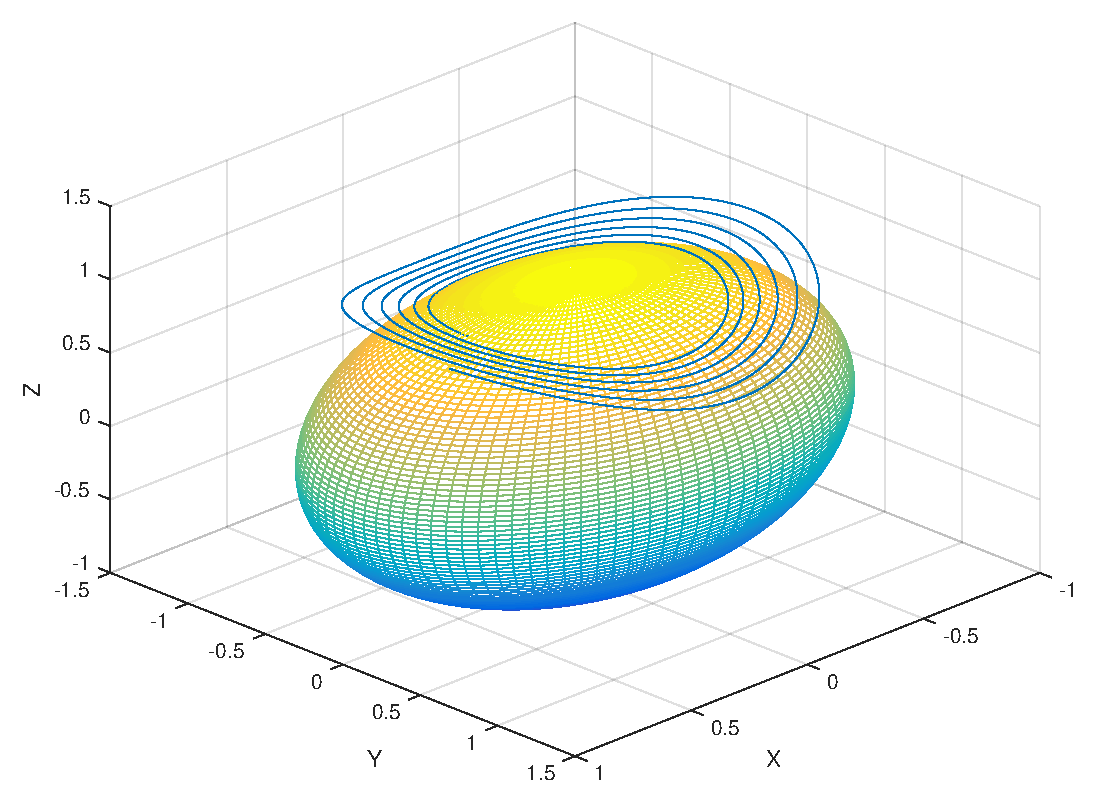
\includegraphics[width=0.7\textwidth]{03/explicit.pdf}
  \caption{非李群方法的数值结果}
  \label{fig:explicit}
\end{figure}

\begin{figure}[h!]
  \centering
  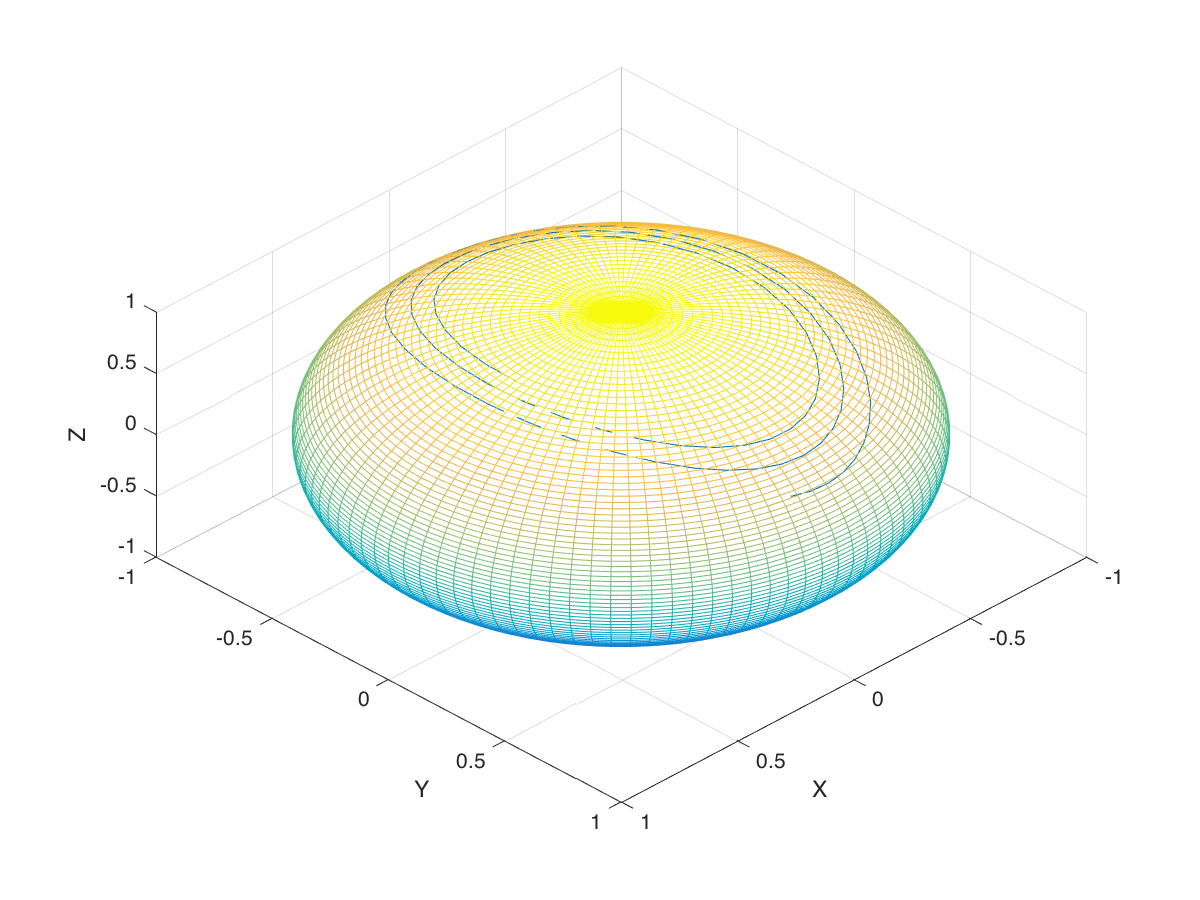
\includegraphics[width=0.7\textwidth]{03/cg2.png}
  \caption{李群方法的数值结果}
  \label{fig:midpoint}
\end{figure}

在本章,我们将用波形松弛方法 \cite{jiang2009wr} 来求解这个哈密尔顿系统 \eqref{eq:hal0}, 波形松弛方法的内容将在 \ref{sec:03wrintro} 中介绍.为了获得更好的数值效果,使用辛方法作为指导工具设计数值格式.

在这里,把结合了辛方法和波形松弛方法的方法叫做\textbf{辛波形松弛方法}.它是传统意义上的波形松弛方法的一个特例,将辛格式作为模型进行逼近,通过运用波形松弛方法解耦的特性,使计算过程更简单.波形松弛方法使问题求解相对隐式方法来说更加容易,同时,辛方法指导了波形松弛方法如何进行解耦.

为了能更好地求解长时间区间的问题,引入窗口加速技术 \cite{jiang2006windowing,ladics2015error}. 窗口技术能够有效地减少波形松弛方法地迭代次数,同时能够保持辛方法的优秀特性.在 \cite{jiang2006windowing} 中作者给出了如何选取窗口长度,另外,窗口技术使得并行求解更加容易 \cite{liu2011waveform}.

接下来,对辛波形松弛方法做进一步地探讨和拓展.该改进基于前面讨论的波形松弛方法对辛格式的改进,更进一步研究波形松弛数值格式在其他保持结构的问题里会有哪些实际可行的应用.对流形上的保结构的数值格式进行波形松弛方法地``改造'',以得到较为容易实现且速度较快的数值格式.

这里我们将给出求解流形上数值方法 RK-MK \cite{arieh2005liegroup} 的一个改进,该方法的``波形松弛化''说明了波形松弛方法在改造数值格式时的意义.这种改造一方面利用了波形松弛方法的解耦,迭代,实现简单等优点,同时还在通过迭代逼近数值格式,保持了原数值格式的优秀特性.

通常来说,我们的数值计算都是在一个空间上进行的,而常用的空间是平直的线性欧式空间.然而,有些方程具有特殊的意义,这些问题的解存在在一个流形上.可是,在全空间上数值计算的误差存在会导致计算结果并不在该流形上.为了解决这一类问题,有一类流形上的李群算法被设计出来,这些算法能够很好地保证数值解落在流形上.上面提到的 RK-MK 算法就是这样一类方法.

然而,即使是李群方法,其数值结果会落到流形上,有些情况也并非令人满意,图 \ref{fig:rkmk2} 中的数值结果虽然保持在流形上了,但是并不是原问题应有的数值解,数值解只是在流形上出现了误差.
\begin{figure}[h!]
  \centering
  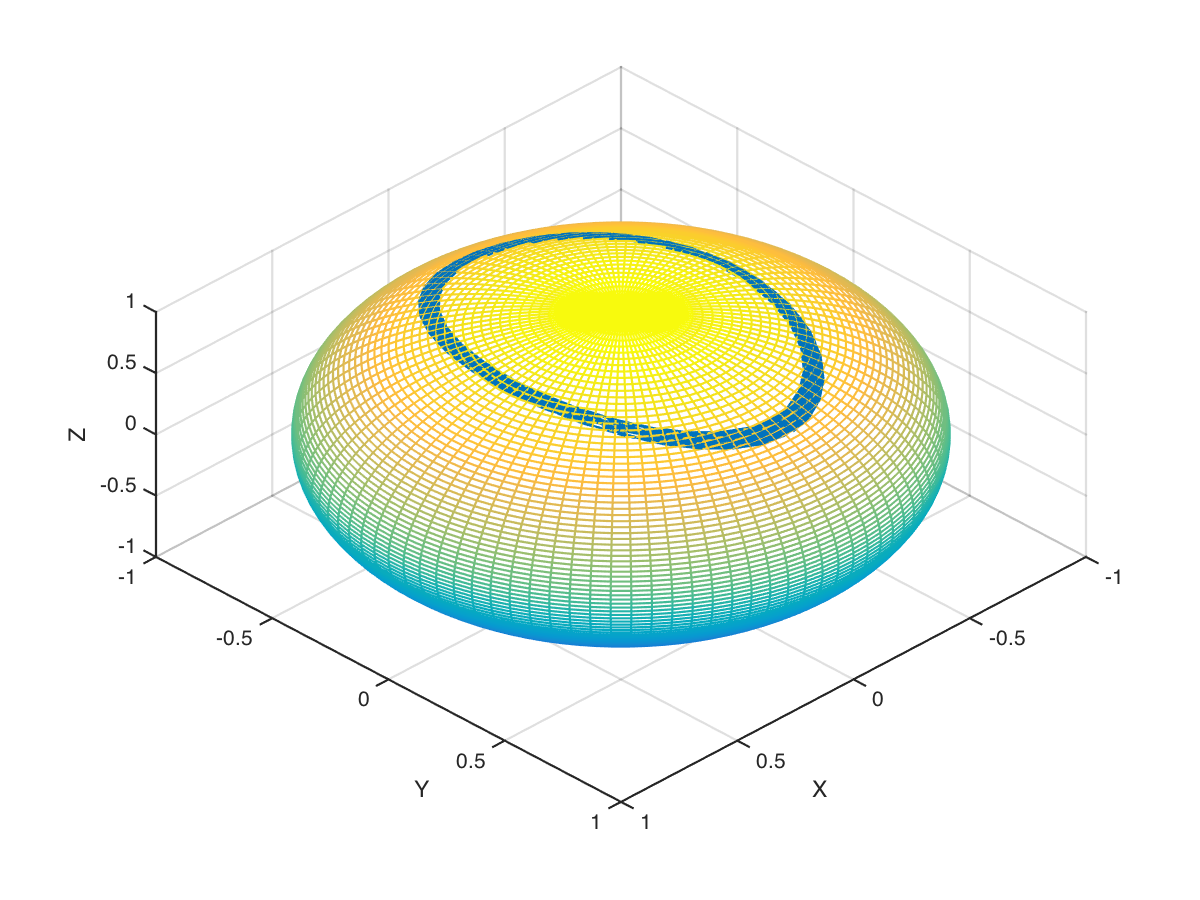
\includegraphics[width=0.7\textwidth]{03/rkmk2.png}
  \caption{较高阶李群方法的数值结果}
  \label{fig:rkmk2}
\end{figure}

根据哈密尔顿系统的理论,事实上,这种偏差可以由类似于辛方法的一类重要的李群方法来解决.根据辛积分理论,辛 Runge-Kutta 方法只有隐式的格式,这里可能需要隐式的 RK-MK 方法才能保持数值解在流形上保结构.

李群方法起初是由 Crouch 和 Grossman \cite{crouch1993numerical} 提出来的,即所谓的 Crouch-Grossman 方法,该方法得到了一系列地推广 \cite{faleinsen2001multi,zaletkin2010numerical,bulychev2001numerical,buono2003numerical,billo1992numerical}. 后来,在 1996 到 1999 年, Munthe-Kaas  等人提出了该方法的一个改进方法 \cite{mk1996lie,mk1997numerical,mk1998runge,mk1999high}, 即 MK-RK 方法,以及后面的一些推广 \cite{ostermann2010exponential,owren2000the,bruls2012lie,munthe2013onpost,garcla2011onalg}. Crouch-Grossman 方法和 MK-RK 方法都用到了李群的指数映射,联结了李群这个流形和李代数之间的关系,并且都利用了 Runge-Kutta 方法这种数值结构,使得阶数可以适当地提高,而且常规意义下的李群方法均为显式方法,计算较为简便.

我们要对隐式的 RK-MK 方法做出一些波形松弛类修正,使得数值方法能够具有较好的长时间稳定性,并且在计算上尽可能地简便,便于实现.该方法的思想来自于上一章对辛方法的波形松弛类改进,和对 RK-MK 方法的理解.在计算过程中,不可避免地要引入窗口技术来加速.

本章的结构如下.首先在小节 \ref{sec:03wrintro} 中,对波形松弛方法进行简单介绍.在小节 \ref{sec:03wrhal} 中,分析了辛波形松弛方法,并给出了以下两个辛波形松弛方法的离散数值格式.同时,分析了系统哈密尔顿函数的守恒性,并介绍了窗口技术的选取问题.在小节 \ref{sec:04wrmani} 中,将对流形上的李群方法进行介绍,并且介绍 Crouch-Grossman 方法与 RK-MK 方法的相关理论,并陈述我们的修正算法.在小节 \ref{sec:03numerical} 中,给出了四个例子来说明问题.最后,做了一个总结.

\section{波形松弛方法基本概念}\label{sec:03wrintro}
\esection{Introduction to the WR Method}

波形松弛方法来源于对大规模集成电路系统的研究 \cite{lelarasmee1982waveform}. 我们认为该方法分为两个部分,分裂和迭代.首先,需要使用分裂函数将大规模的系统划分为较小规模的子系统.接下来是迭代,迭代的过程先分别求解子系统,再在系统之间交换信息,进行下一次迭代,直到收敛.由此可见,波形松弛方法的显著特性是问题解耦和潜在的可并行性.

波形松弛方法给我们指出了一种不同的求解微分方程的迭代方式.它不是简简单单的通过求解离散过后的代数方程组的松弛方法,而是通过对方程分裂而构造出来的一种函数迭代方法,是``波形''的迭代.考虑如下的一阶常微分方程
\begin{equation}\label{eq:03ode}
\left\{
\begin{aligned}
\frac{dx(t)}{dt}&=f(x(t),t),\\
x(0)&=x_{0}.
\end{aligned}
\right.
\end{equation}

波形松弛方法的基本思想是找到一个分裂函数 $F(u,v,t)$ 满足 $F(u,u,t)=f(u,t)$, 这样如下方程
\begin{equation*}
\left\{
\begin{aligned}
\frac{dx^{k+1}(t)}{dt}&=F(x^{k+1}(t),x^{k}(t),t),\\
x^{k+1}(0)&=x_{0},
\end{aligned}
\right.
\end{equation*}
就能够快速求解并且更容易求解.不能逃避的一件事情是,在分裂函数 $F(u,v,t)$ 下,迭代后的函数序列 $x^{k}(t)$ 要收敛到原方程 \eqref{eq:03ode} 的解.

波形松弛方法的一个优点是能够把耦合的系统,通过分裂,在迭代过程中化为非耦合的系统,即解耦,对于一些问题来讲,这为算法的并行计算提供了条件.同时,注意到,在计算的过程中,波形松弛方法能够将一些只能隐式格式求解的问题,化为显式或者半隐式的格式即可求解的问题.

一些常见的分裂函数取法有 Gauss-Jacobi 波形松弛方法, Gauss-Seidel 波形松弛方法,等等.作为一个例子,如果记 $u=(u_{1},u_{2},\ldots,u_{n})^{T}, v=(v_{1},v_{2},\ldots,v_{n})^{T}$, 并且方程的形式为
\begin{equation*}
\left\{
\begin{aligned}
\frac{dx_{1}(t)}{dt}&=f_{1}(x_{1}(t),x_{2}(t),\ldots,x_{n}(t),t),\\
\frac{dx_{2}(t)}{dt}&=f_{2}(x_{1}(t),x_{2}(t),\ldots,x_{n}(t),t),\\
\ldots&\ldots\ldots\ldots\ldots\ldots\ldots\\
\frac{dx_{n}(t)}{dt}&=f_{n}(x_{1}(t),x_{2}(t),\ldots,x_{n}(t),t),\\
x_{1}(0)&=x_{1,0},x_{2}(0)=x_{2,0},\ldots,x_{n}(0)=x_{n,0},
\end{aligned}
\right.
\end{equation*}
Gauss-Jacobi 波形松弛方法和 Gauss-Seidel 波形松弛方法的分裂函数分别为
\begin{align}\label{eq:wr}
&F_{i}(u,v,t)=f_{i}(v_{1},v_{2},\ldots,v_{i-1},u_{i},v_{i+1},\ldots,v_{n},t)\quad \text{(Gauss-Jacobi~WR)},\\
&F_{i}(u,v,t)=f_{i}(u_{1},u_{2},\ldots,u_{i-1},u_{i},v_{i+1},\ldots,v_{n},t)\quad \text{(Gauss-Seidel~WR)}.
\end{align}

简而言之,波形松弛方法 \cite{jiang2009wr} 作为一个数学工具,思想起源于大规模集成电路的求解方法.当系统的规模大到一定程度的时候,使用现有的计算资源求解该问题就变得困难,可以通过分裂成更易于求解的小型系统来计算.为了达到这个目标,选取分裂函数 $F(z,y)$ 使得 $F(z,z)=f(z)$, 然后将方程 \eqref{eq:hal0} 中的 $f(z)$ 替换为 $F(z,y)$. 接下来为每一个子系统选择一个合适的初始迭代,将 $F(z,y)$ 中的 $y$ 作为已知函数, $z$ 作为未知函数,这样每次迭代的计算量就降低了.然而,由于初值的选取和格式的设计,这样的一步计算不会得到系统的真实解.这要通过迭代来保证收敛到方程的真解.通常将迭代方程记作 $\dot{z}^{k+1}=F(z^{k+1},z^{k})$, 其中 $k=0,1,\cdots$ 是迭代次数.


\section{哈密尔顿系统的辛波形松弛方法}\label{sec:03wrhal}
\esection{Symplectic WR Methods for Hamiltonian Systems}
在本小节,我们分析哈密尔顿系统 \eqref{eq:hal0} 的辛波形松弛方法.把方程 \eqref{eq:hal0} 写成如下形式
\begin{equation}\label{eq:hal1}
\dot{z}=f(z),
\end{equation}
式中 $z=(q,p)^T$ 为区间 $[0,T]$ 上的未知函数, $f(z)$ 是方程 \eqref{eq:hal0} 右端函数.

对于波形松弛方法,需要取一个分裂函数 $F(x,y)$ 使得 $F(z,z)=f(z)$. 该分裂函数用于对系统 \eqref{eq:hal1} 进行解耦.对波形松弛方法,有如下的结果.

\begin{theorem}[\cite{jiang2009wr}]\label{thm:wr}
	\emph{如果 \eqref{eq:hal1} 的分裂函数 $F(x,y)$ 对变量 $x$ 和 $y$ 是 Lipschitz 连续的,那么波形松弛方法收敛.}
\end{theorem}

\subsection{连续时间的辛波形松弛方法}
\esubsection{The Continuous-time Symplectic WR Method}
辛波形松弛方法属于传统波形松弛方法的特例.所以定理 \ref{thm:wr} 自动成立.接下来,我们进一步研究哈密尔顿函数 $H$ 的变化情况.

\begin{theorem}
\emph{如果辛波形松弛方法收敛,并且 \eqref{eq:hal1} 里的右端函数 $f$ 有界,则哈密尔顿函数收敛到常函数.}
\end{theorem}

{\textbf{证明}} 记 $H_0$ 为系统的哈密尔顿函数.因为该哈密尔顿 $H_0$ 为常函数,有
\begin{equation*}
\frac{dH_0}{dt}=0.
\end{equation*}
记 $H^{k+1}$ 为第 $k+1$ 此迭代的哈密尔顿函数,即
\begin{equation*}
H^{k+1}=H(q^{k+1},p^{k+1}),
\end{equation*}
式中 $q^{k+1}$ 和 $p^{k+1}$ 为第 $k+1$ 步的位移和动量函数.

接下来,来看函数 $H^{k+1}-H_0$ 的导数.
\begin{equation*}
\begin{aligned}
\frac{d(H^{k+1}-H_0)}{dt}=&H_q(z^{k+1})^TF_1(z^{k+1},z^{k})-H_q(z)^TF_1(z,z)\\
&+H_p(z^{k+1})^TF_2(z^{k+1},z^{k})-H_p(z)^TF_2(z,z),
\end{aligned}
\end{equation*}
式中 $F_1$ 和 $F_2$ 分别是 $H_p$ 和 $-H_q$ 的分裂函数.

于是,有
\begin{equation*}
\begin{aligned}
\|H_q(z^{k+1})^TF_1(z^{k+1},z^{k})&-H_q(z)^TF_1(z,z)\|\\
&=\|H_q(z^{k+1})^TF_1(z^{k+1},z^{k})-H_q(z)^TF_1(z^{k+1},z^{k})\\
&+H_q(z)^TF_1(z^{k+1},z^{k})-H_q(z)^TF_1(z,z^{k})\\
&+H_q(z)^TF_1(z,z^{k})-H_q(z)^TF_1(z,z)\|\\
&\le\|H_q(z^{k+1})^TF_1(z^{k+1},z^{k})-H_q(z)^TF_1(z^{k+1},z^{k})\|\\
&+\|H_q(z)^TF_1(z^{k+1},z^{k})-H_q(z)^TF_1(z,z^{k})\|\\
&+\|H_q(z)^TF_1(z,z^{k})-H_q(z)^TF_1(z,z)\|\\
&\le A_1\|z^{k+1}-z\|+B_1\|z^{k}-z\|,
\end{aligned}
\end{equation*}
式中 $A_1$ 和 $B_1$ 是常数.

类似地,有
\begin{equation*}
\|H_q(z^{k+1})^TF_1(z^{k+1},z^{k})-H_q(z)^TF_1(z,z)\|\le A_2\|z^{k+1}-z\|+B_2\|z^{k}-z\|,
\end{equation*}
式中 $A_2$ 和 $B_2$ 是常数.

因此
\begin{equation*}
\frac{d\|H^{k+1}-H_0\|}{dt}\le (A_1+A_2)\|z^{k+1}-z\|+(B_1+B_2)\|z^{k}-z\| \to 0.
\end{equation*}

上面最后一个等号成立是因为波形松弛方法的收敛性.注意到 $H^{k+1}(z(0))=H_0(z(0))$, 定理即可获得证明.

证毕.

\subsection{离散时间的辛波形松弛方法}
\esubsection{The Discrete-time Symplectic WR Method}
离散的数值格式并不能够很直接地看出来.为了构造离散格式,必须同时兼顾辛格式和分裂函数.假设一个单步的辛格式为
\begin{equation*}
z_{n+1}=z_{n}+h g(z_{n+1},z_{n}),
\end{equation*}
其相应的辛波形松弛方法即为
\begin{equation}\label{eq:discrete}
z_{n+1}^{k+1}=z_{n}^{k+1}+h \tilde{F}(z_{n+1}^{k+1},z_{n+1}^{k},z_{n}^{k+1},z_{n}^{k}),
\end{equation}
式中 $\tilde{F}(x,y,x,y)=F(x,y)$ 和 $\tilde{F}(x,x,y,y)=g(x,y)$.

\begin{theorem}
\emph{如果辛波形松弛方法收敛,并且辛格式对变量 $z_{n}$ 和 $z_{n+1}$ Lipschitz 连续,那么辛波形松弛方法的哈密尔顿函数收敛到离散格式的哈密尔顿函数.}
\end{theorem}

{\textbf{证明}} 记 $H^{k+1}_{n+1}$ 为 $H(z_{n+1}^{k+1})$, $H_{n+1}$ 为 $H(z_{n+1})$ 其中 $z_{n+1}^{k+1}$ 和 $z_{n+1}$ 分别为辛波形松弛方法和辛方法的数值解.

说离散的辛波形松弛方法是收敛的,如果满足 $\|z_{n+1}^{k+1} - z_{n+1}\| \to 0~(k \to \infty)$.

注意到
\begin{equation*}
\begin{aligned}
\|H^{k+1}_{n+1}-H_{n+1}\|&=\|H(z_{n}^{k+1}+h \tilde{F}(z_{n+1}^{k+1},z_{n+1}^{k},z_{n}^{k+1},z_{n}^{k}))-H(z_{n+1})\|\\
&\le \|\tilde{H}(z_{n+1}^{k+1},z_{n+1}^{k},z_{n}^{k+1},z_{n}^{k})-\tilde{H}(z_{n+1},z_{n+1}^{k},z_{n}^{k+1},z_{n}^{k})\|\\
&+\|\tilde{H}(z_{n+1},z_{n+1}^{k},z_{n}^{k+1},z_{n}^{k})-\tilde{H}(z_{n+1},z_{n+1},z_{n}^{k+1},z_{n}^{k})\|\\
&+\|\tilde{H}(z_{n+1},z_{n+1},z_{n}^{k+1},z_{n}^{k})-\tilde{H}(z_{n+1},z_{n+1},z_{n},z_{n}^{k})\|\\
&+\|\tilde{H}(z_{n+1},z_{n+1},z_{n},z_{n}^{k})-\tilde{H}(z_{n+1},z_{n+1},z_{n},z_{n})\|\\
&+\|\tilde{H}(z_{n+1},z_{n+1},z_{n},z_{n})-H(z_{n+1})\|,\\
\end{aligned}
\end{equation*}
式中 $\tilde{H}(x,y,z,w)=z+h \tilde{F}(x,y,z,w)$ 为数值辛格式,所以有
\begin{equation*}
\tilde{H}(z_{n+1},z_{n+1},z_{n},z_{n})=H(z_{n+1}).
\end{equation*}

因此,有
\begin{equation*}
\|H^{k+1}_{n+1}-H_{n+1}\|\le C(\|z_{n+1}^{k+1}-z_{n+1}\|+ \|z_{n+1}^{k}-z_{n+1}\|+ \|z_{n}^{k+1}-z_{n}\|+ \|z_{n}^{k}-z_{n}\|),
\end{equation*}
式中 $C$ 为常数.上面的不等式表明 $\|H^{k+1}_{n+1}-H_{n+1}\| \to 0$ 随着 $k \to \infty$.

证毕.

\subsubsection{辛欧拉波形松弛方法}
\esubsubsection{Symplectic Euler Waveform Relaxation Method}
对于哈密尔顿函数 \eqref{eq:hal0} 和辛欧拉方法 \cite{hairer2014challenges}
\begin{equation}\label{eq:symeuler1}
  \begin{array}{c}
    q_{n+1}=q_{n}+hH_{p}(q_{n},p_{n+1}),\\
    p_{n+1}=p_{n}-hH_{q}(q_{n},p_{n+1}).
  \end{array}
\end{equation}

将 Jacobi 波形松弛方法作为分裂函数,有
\begin{equation*}
  \left\{
    \begin{aligned}
      q_{1,n+1}^{(k+1)}&=q_{1,n}^{(k+1)}+hH_{p_{1}}(q_{1,n}^{(k+1)},q_{2,n}^{(k)},\ldots,q_{d,n}^{(k)},p_{1,n+1}^{(k)},p_{2,n+1}^{(k)},\ldots,p_{d,n+1}^{(k)}),\\
      q_{2,n+1}^{(k+1)}&=q_{2,n}^{(k+1)}+hH_{p_{2}}(q_{1,n}^{(k)},q_{2,n}^{(k+1)},\ldots,q_{d,n}^{(k)},p_{1,n+1}^{(k)},p_{2,n+1}^{(k)},\ldots,p_{d,n+1}^{(k)}),\\
      \ldots&\ldots\ldots\ldots\ldots\ldots\ldots\\
      q_{d,n+1}^{(k+1)}&=q_{d,n}^{(k+1)}+hH_{p_{d}}(q_{1,n}^{(k)},q_{2,n}^{(k)},\ldots,q_{d,n}^{(k+1)},p_{1,n+1}^{(k)},p_{2,n+1}^{(k)},\ldots,p_{d,n+1}^{(k)}),\\
      p_{1,n+1}^{(k+1)}&=p_{1,n}^{(k+1)}-hH_{q_{1}}(q_{1,n}^{(k)},q_{2,n}^{(k)},\ldots,q_{d,n}^{(k)},p_{1,n+1}^{(k+1)},p_{2,n+1}^{(k)},\ldots,p_{d,n+1}^{(k)}),\\
      p_{2,n+1}^{(k+1)}&=p_{2,n}^{(k+1)}-hH_{q_{2}}(q_{1,n}^{(k)},q_{2,n}^{(k)},\ldots,q_{d,n}^{(k)},p_{1,n+1}^{(k)},p_{2,n+1}^{(k+1)},\ldots,p_{d,n+1}^{(k)}),\\
      \ldots&\ldots\ldots\ldots\ldots\ldots\ldots\\
      p_{d,n+1}^{(k+1)}&=p_{d,n}^{(k+1)}-hH_{q_{d}}(q_{1,n}^{(k)},q_{2,n}^{(k)},\ldots,q_{d,n}^{(k)},p_{1,n+1}^{(k)},p_{2,n+1}^{(k)},\ldots,p_{d,n+1}^{(k+1)}).\\
    \end{aligned}
  \right.
\end{equation*}
如果 $p,q \in \mathbb{R}$, 那么上面的方法化为
\begin{equation}\label{eq:schemejacobi}
  \begin{aligned}
    q_{n+1}^{(k+1)}&=q_{n}^{(k+1)}+hH_{p}(q_{n}^{(k+1)},p_{n+1}^{(k)}),\\
    p_{n+1}^{(k+1)}&=p_{n}^{(k+1)}-hH_{q}(q_{n}^{(k)},p_{n+1}^{(k+1)}).
  \end{aligned}
\end{equation}
类似地,使用 Gauss-Seidel WR 波形松弛方法作为分裂函数,有
\begin{equation*}
  \left\{
    \begin{aligned}
      q_{1,n+1}^{(k+1)}&=q_{1,n}^{(k+1)}+hH_{p_{1}}(q_{1,n}^{(k+1)},q_{2,n}^{(k)},\ldots,q_{d,n}^{(k)},p_{1,n+1}^{(k)},p_{2,n+1}^{(k)},\ldots,p_{d,n+1}^{(k)}),\\
      q_{2,n+1}^{(k+1)}&=q_{2,n}^{(k+1)}+hH_{p_{2}}(q_{1,n}^{(k+1)},q_{2,n}^{(k+1)},\ldots,q_{d,n}^{(k)},p_{1,n+1}^{(k)},p_{2,n+1}^{(k)},\ldots,p_{d,n+1}^{(k)}),\\
      \ldots&\ldots\ldots\ldots\ldots\ldots\ldots\\
      q_{d,n+1}^{(k+1)}&=q_{d,n}^{(k+1)}+hH_{p_{d}}(q_{1,n}^{(k+1)},q_{2,n}^{(k+1)},\ldots,q_{d,n}^{(k+1)},p_{1,n+1}^{(k)},p_{2,n+1}^{(k)},\ldots,p_{d,n+1}^{(k)}),\\
      p_{1,n+1}^{(k+1)}&=p_{1,n}^{(k+1)}-hH_{q_{1}}(q_{1,n}^{(k+1)},q_{2,n}^{(k+1)},\ldots,q_{d,n}^{(k+1)},p_{1,n+1}^{(k+1)},p_{2,n+1}^{(k)},\ldots,p_{d,n+1}^{(k)}),\\
      p_{2,n+1}^{(k+1)}&=p_{2,n}^{(k+1)}-hH_{q_{2}}(q_{1,n}^{(k+1)},q_{2,n}^{(k+1)},\ldots,q_{d,n}^{(k+1)},p_{1,n+1}^{(k+1)},p_{2,n+1}^{(k+1)},\ldots,p_{d,n+1}^{(k)}),\\
      \ldots&\ldots\ldots\ldots\ldots\ldots\ldots\\
      p_{d,n+1}^{(k+1)}&=p_{d,n}^{(k+1)}-hH_{q_{d}}(q_{1,n}^{(k+1)},q_{2,n}^{(k+1)},\ldots,q_{d,n}^{(k+1)},p_{1,n+1}^{(k+1)},p_{2,n+1}^{(k+1)},\ldots,p_{d,n+1}^{(k+1)}).
    \end{aligned}
  \right.
\end{equation*}
如果 $p,q \in \mathbb{R}$, 则上面的方法化为
\begin{equation}\label{eq:schemegauss}
  \begin{aligned}
    q_{n+1}^{(k+1)}&=q_{n}^{(k+1)}+hH_{p}(q_{n}^{(k+1)},p_{n+1}^{(k)}),\\
    p_{n+1}^{(k+1)}&=p_{n}^{(k+1)}-hH_{q}(q_{n}^{(k+1)},p_{n+1}^{(k+1)}).
  \end{aligned}
\end{equation}

从形式上来看,如果忽略下角标 $p$ 和 $q$, 这个格式可以看成波形松弛方法,如果忽略上角标则可以看成是辛欧拉方法.

\subsubsection{辛 Runge-Kutta 波形松弛方法}
\esubsubsection{The Symplectic Runge-Kutta WR Method}
对于 Runge-Kutta 方法,使用了一个将 Runge-Kutta 方法和波形松弛方法结合的策略 \cite{bellen1993use,bellen1994contractivity}. 可以知道, $\nu$ 步的 Runge-Kutta 方法可以写成
\begin{equation*}
  \left\lbrace
    \begin{aligned}
      Y_{n+1}^{r}&=\eta(t_{n})+h\sum_{s=1}^{\nu}a_{rs}f(t_{n+1}^{s},Y_{n+1}^{s}),\quad r=1,\cdots, \nu, \\
      \eta(t_{n+1})&=\eta(t_{n})+h\sum_{s=1}^{\nu}b_{s}f(t_{n+1}^{s},Y_{n+1}^{s}).
    \end{aligned}
  \right.
\end{equation*}

其对应的 Butcher 表可以写成

\begin{center}
  \begin{tabular}{c|cccc}
    $c_1$&$a_{11}$&$a_{12}$&$\cdots$&$a_{1\nu}$\\
    $c_2$&$a_{21}$&$a_{22}$&$\cdots$&$a_{2\nu}$\\
    $\vdots$&$\vdots$&$\vdots$&$\ddots$&$\vdots$\\
    $c_{\nu}$&$a_{\nu 1}$&$a_{\nu 2}$&$\cdots$&$a_{\nu \nu}$\\
    \hline
         &$b_{1}$&$b_{2}$&$\cdots$&$b_{\nu}$
  \end{tabular}
\end{center}

如果该 Runge-Kutta 的 Butcher 表满足
\begin{equation*}
  b_ia_{ij}+b_ja_{ji}=b_ib_j,\quad \textrm{对所有}\,\, i,j=1,2,\cdots,\nu,
\end{equation*}
则该 Runge-Kutta 方法是保辛的.

这里,采用如下的辛波形松弛方法 \cite{bellen1993use}
\begin{equation*}
  \left\lbrace
    \begin{aligned}
      Y_{n+1}^{r,(k+1)}&=\eta^{(k+1)}(t_{n})+h\sum_{s=1}^{\nu}a_{rs}F(t_{n+1}^{s},Y_{n+1}^{s,(k+1)},Y_{n+1}^{s,(k)}),\quad r=1,\cdots, \nu, \\
      \eta^{(k+1)}(t_{n+1})&=\eta^{(k+1)}(t_{n})+h\sum_{s=1}^{\nu}b_{s}F(t_{n+1}^{s},Y_{n+1}^{s,(k+1)},Y_{n+1}^{s,(k)}).
    \end{aligned}
  \right.
\end{equation*}

根据构造辛波形松弛方法的策略,可以将 Gauss-Jacobi~波形松弛方法 (WRGJ),和 Gauss-Seidel~波形松弛方法(WRGS) 应用于 Runge-Kutta方法,得到相应的 WRGJRK 和 WRGSRK 方法.

所以 WRGJRK 方法为, 对于 $i=1,\cdots,2d$
\begin{equation*}
  \left\lbrace
    \begin{aligned}
      Y_{r,i}^{(k+1)}=&\eta_{i}^{(k+1)}(t_{n})+h\sum_{s=1}^{\nu}a_{rs}f_i(t_{n+1}^{s},Y_{s,1}^{(k)},\cdots,\\
      &Y_{s,i-1}^{(k)},Y_{s,i}^{(k+1)},Y_{s,i+1}^{(k)},\cdots,Y_{s,2d}^{(k)}),\quad r=1,\cdots, \nu, \\
      \eta_{i}^{(k+1)}(t_{n+1})=&\eta_{i}^{(k+1)}(t_{n})+h\sum_{s=1}^{\nu}b_{s}f_i(t_{n+1}^{s},Y_{s,1}^{(k)},\cdots,\\
      &Y_{s,i-1}^{(k)},Y_{s,i}^{(k+1)},Y_{s,i+1}^{(k)},\cdots,Y_{s,2d}^{(k)}).
    \end{aligned}
  \right.
\end{equation*}

WRGSRK 方法为, 对于 $i=1,\cdots,2d$
\begin{equation*}
  \left\lbrace
    \begin{aligned}
      Y_{r,i}^{(k+1)}=&\eta_{i}^{(k+1)}(t_{n})+h\sum_{s=1}^{\nu}a_{rs}f_i(t_{n+1}^{s},Y_{s,1}^{(k+1)},\cdots,\\
      &Y_{s,i-1}^{(k+1)},Y_{s,i}^{(k+1)},Y_{s,i+1}^{(k)},\cdots,Y_{s,2d}^{(k)}),\quad r=1,\cdots, \nu, \\
      \eta_{i}^{(k+1)}(t_{n+1})=&\eta_{i}^{(k+1)}(t_{n})+h\sum_{s=1}^{\nu}b_{s}f_i(t_{n+1}^{s},Y_{s,1}^{(k+1)},\cdots,\\
      &Y_{s,i-1}^{(k+1)},Y_{s,i}^{(k+1)},Y_{s,i+1}^{(k)},\cdots,Y_{s,2d}^{(k)}).
    \end{aligned}
  \right.
\end{equation*}

把这些方法作用于哈密尔顿系统,有如下的 WRGJRK 格式, 对于 $i=1,\cdots,d$, $r=1,\cdots,\nu$
\begin{equation}\label{eq:schemerkjacobi}
  \left\lbrace
    \begin{aligned}
      Q_{r,i}^{(k+1)}&=q_{i}^{(k+1)}(t_{n})+h\sum_{s=1}^{\nu}a_{rs}H_{p,i}(Q_{s,1}^{(k)},\cdots,Q_{s,i-1}^{(k)},\\
                            &Q_{s,i}^{(k+1)},Q_{s,i+1}^{(k)},\cdots,Q_{s,d}^{(k)},P_{s,1}^{(k)},\cdots,P_{s,d}^{(k)}),\\
      P_{r,i}^{(k+1)}&=p_{i}^{(k+1)}(t_{n})-h\sum_{s=1}^{\nu}a_{rs}H_{q,i}(Q_{s,1}^{(k)},\cdots,Q_{s,d}^{(k)},\\
                            &P_{s,1}^{(k)},\cdots,P_{s,i-1}^{(k)},P_{s,i}^{(k+1)},P_{s,i+1}^{(k)}\cdots,P_{s,d}^{(k)}),\\
      q_{i}^{(k+1)}(t_{n+1})&=q_{i}^{(k+1)}(t_{n})+h\sum_{s=1}^{\nu}b_{s}H_{p,i}(Q_{s,1}^{(k)},\cdots,Q_{s,i-1}^{(k)},\\
                            &Q_{s,i}^{(k+1)},Q_{s,i+1}^{(k)},\cdots,Q_{s,d}^{(k)},P_{s,1}^{(k)},\cdots,P_{s,d}^{(k)}),\\
      p_{i}^{(k+1)}(t_{n+1})&=p_{i}^{(k+1)}(t_{n})-h\sum_{s=1}^{\nu}b_{s}H_{q,i}(Q_{s,1}^{(k)},\cdots,Q_{s,d}^{(k)},\\
                            &P_{s,1}^{(k)},\cdots,P_{s,i-1}^{(k)},P_{s,i}^{(k+1)},P_{s,i+1}^{(k)}\cdots,P_{s,d}^{(k)}),\\
    \end{aligned}
  \right.
\end{equation}

和 WRGSRK 格式, 对于 $i=1,\cdots,d$, $r=1,\cdots,\nu$
\begin{equation*}
  \left\lbrace
    \begin{aligned}
      Q_{r,i}^{(k+1)}&=q_{i}^{(k+1)}(t_{n})+h\sum_{s=1}^{\nu}a_{rs}H_{p,i}(Q_{s,1}^{(k+1)},\cdots,Q_{s,i-1}^{(k+1)},\\
                            &Q_{s,i}^{(k+1)},Q_{s,i+1}^{(k)},\cdots,Q_{s,d}^{(k)},P_{s,1}^{(k)},\cdots,P_{s,d}^{(k)}),\\
      P_{r,i}^{(k+1)}&=p_{i}^{(k+1)}(t_{n})-h\sum_{s=1}^{\nu}a_{rs}H_{q,i}(Q_{s,1}^{(k+1)},\cdots,Q_{s,d}^{(k+1)},\\
                            &P_{s,1}^{(k+1)},\cdots,P_{s,i-1}^{(k+1)},P_{s,i}^{(k+1)},P_{s,i+1}^{(k)}\cdots,P_{s,d}^{(k)}),\\
      q_{i}^{(k+1)}(t_{n+1})&=q_{i}^{(k+1)}(t_{n})+h\sum_{s=1}^{\nu}b_{s}H_{p,i}(Q_{s,1}^{(k+1)},\cdots,Q_{s,i-1}^{(k+1)},\\
                            &Q_{s,i}^{(k+1)},Q_{s,i+1}^{(k)},\cdots,Q_{s,d}^{(k)},P_{s,1}^{(k)},\cdots,P_{s,d}^{(k)}),\\
      p_{i}^{(k+1)}(t_{n+1})&=p_{i}^{(k+1)}(t_{n})-h\sum_{s=1}^{\nu}b_{s}H_{q,i}(Q_{s,1}^{(k+1)},\cdots,Q_{s,d}^{(k+1)},\\
                            &P_{s,1}^{(k+1)},\cdots,P_{s,i-1}^{(k+1)},P_{s,i}^{(k+1)},P_{s,i+1}^{(k)}\cdots,P_{s,d}^{(k)}).\\
    \end{aligned}
  \right.
\end{equation*}

\subsection{离散时间的辛波形松弛方法的进一步讨论}
\esubsection{Further Discussions on the Discrete-time Symplectic WR Method}
接下来,对格式 \eqref{eq:schemejacobi} 做出简要分析.格式 \eqref{eq:schemegauss} 可以给出类似的结果.

对于波形松弛方法来说,需要给出一个初始猜测 $q_{i}^{(0)},~p_{i}^{(0)}~\text{for}~i=0,1,\ldots,N$, 其中 $i$ 是时间网格的指标.选定了初始迭代之后,就得到了如下的波形松弛格式的算法.通常来说,初始迭代可以取作 $q_{i}^{(0)}=q_{0},~p_{i}^{(0)}=p_{0}.$

\begin{algorithm}
\caption{辛欧拉波形松弛方法}
\label{alg:alg1}
\begin{algorithmic}
    \STATE 设置初始迭代值 $q_{i}^{(0)}, p_{i}^{(0)} \text{for}~i=0,1,\ldots,N.$
    \WHILE{达到容许的误差}
        \STATE 使用数值格式 \eqref{eq:schemejacobi}, 用 $q^{(k)},~p^{(k)}$ 求解 $q^{(k+1)},~p^{(k+1)}$.
    \ENDWHILE
\end{algorithmic}
\end{algorithm}


\begin{theorem}[算法 \eqref{alg:alg1} 的收敛性]\label{thm:sj}\\
\emph{如果 $H_{p}$ 和 $H_{q}$ 对变量 $p$ 和 $q$ Lipschitz 连续,即,
\begin{equation*}
  \begin{aligned}
    \|H_{p}(q_{1},p)-H_{p}(q_{2},p)\| &\le M_{q} \|q_{1}-q_{2}\|, \\
    \|H_{p}(q,p_{1})-H_{p}(q,p_{2})\| &\le M_{p} \|p_{1}-p_{2}\|, \\
    \|H_{q}(q_{1},p)-H_{q}(q_{2},p)\| &\le L_{q} \|q_{1}-q_{2}\|, \\
    \|H_{q}(q,p_{1})-H_{q}(q,p_{2})\| &\le L_{p} \|p_{1}-p_{2}\|, \\
  \end{aligned}
\end{equation*}
那么格式 \eqref{eq:schemejacobi} 收敛.}
\end{theorem}

{\textbf{证明}} 记 $\epsilon_{q,n}^{(k)}=q_{n}^{(k)}-q_{n}$ 和 $\epsilon_{p,n}^{(k)}=p_{n}^{(k)}-p_{n}$, 然后将式 \eqref{eq:schemejacobi} 和 \eqref{eq:symeuler1} 相减,得到
  \begin{equation*}
    \begin{aligned}
      \epsilon_{q,n+1}^{(k+1)}&=\epsilon_{q,n}^{(k+1)}+h(H_{p}(q_{n}^{(k+1)},p_{n+1}^{(k)})-H_{p}(q_{n},p_{n+1})),\\
      \epsilon_{p,n+1}^{(k+1)}&=\epsilon_{p,n}^{(k+1)}-h(H_{q}(q_{n}^{(k)},p_{n+1}^{(k+1)})-H_{q}(q_{n},p_{n+1})).
    \end{aligned}
  \end{equation*}
  然后,记 $e_{p,n}^{k}=\|\epsilon_{p,n}^{(k)}\|$, 然后应用 Lipschitz 条件,有
  \begin{equation*}
    \begin{aligned}
      e_{q,n+1}^{k+1}&\le e_{q,n}^{k+1}+hM_{q}e_{q,n}^{k+1}+hM_{p}e_{p,n+1}^{k},\\
      e_{p,n+1}^{k+1}&\le e_{p,n}^{k+1}+hL_{q}e_{q,n}^{k}+hL_{p}e_{p,n+1}^{k+1}.
    \end{aligned}
  \end{equation*}
  令 $\alpha=\frac{1}{1-hL_{p}}$, $\beta=\frac{hL_{q}}{1-hL_{p}}$, $\gamma=1+hM_{q}$ 和 $\theta=hM_{p}$, 有
  \begin{equation*}
    \begin{aligned}
      e_{q,n+1}^{k+1}&\le \gamma e_{q,n}^{k+1}+\theta e_{p,n+1}^{k},\\
      e_{p,n+1}^{k+1}&\le \alpha e_{p,n}^{k+1}+\beta e_{q,n}^{k}.
    \end{aligned}
  \end{equation*}
  注意到 $e_{q,0}^{k}=0, e_{p,0}^{k}=0$, 能够得到
  \begin{equation*}
    \begin{aligned}
      e_{q,n+1}^{k+1}&\le \gamma^{n}\theta e_{p,1}^{k}+\gamma^{n-1}\theta e_{p,2}^{k}+\ldots+\gamma \theta e_{p,n}^{k}+\theta e_{p,n+1}^{k},\\
      e_{p,n+1}^{k+1}&\le \alpha^{n-1}\beta e_{q,1}^{k}+\alpha^{n-2}\beta e_{q,2}^{k}+\ldots+\alpha \beta
      e_{q,n-1}^{k}+\beta e_{q,n}^{k}.
    \end{aligned}
  \end{equation*}
  为了记号简单,把上面的不等式写作
  \begin{equation*}
    \begin{aligned}
      e_{q,n+1}^{k+1}&\le \sum_{a+b=n+1}\gamma^{a}\theta e_{p,b}^{k},\\
      e_{p,n+1}^{k+1}&\le \sum_{a+b=n}\alpha^{a}\beta e_{q,b}^{k}.
    \end{aligned}
  \end{equation*}
  然后得到
  \begin{equation*}
    \begin{aligned}
      e_{q,n+1}^{k+1}&\le \beta\theta \sum_{a+b+c=n}\alpha^{a}\gamma^{b} e_{q,c}^{k-1},\\
      e_{p,n+1}^{k+1}&\le \beta \theta \sum_{a+b+c=n}\alpha^{a}\gamma^{b} e_{p,c}^{k-1}.
    \end{aligned}
  \end{equation*}
  上面的两个不等式有相同的形式,所以将其记作
  \begin{equation*}
    e_{n+1}^{k+1}\le \beta \theta \sum_{a+b+c=n}\alpha^{a}\gamma^{b} e_{c}^{k-1},
  \end{equation*}
  式中 $e_{n+1}^{k+1}$ 代表 $e_{p,n+1}^{k+1}$ 或 $e_{q,n+1}^{k+1}$. 如果 $k+1=2t$, 那么有
  \begin{equation*}
    e_{n+1}^{k+1}\le \beta^{t} \theta^{t} \sum_{a+b+c=n-t+1}\alpha^{a}\gamma^{b} e_{c}^{0}.
  \end{equation*}
  由于 $c\le n-t+1$, $e_{n+1}^{k+1}$ 随着 $t$ 的增长,依赖的 $e_{s}^{0}, (s= 1,2,\ldots)$ 越来越少,可以看到该算法收敛.

证毕.

\begin{theorem}\label{thm:sym}
\emph{假设 $H_q$ 和 $H_p$ 是有界的,那么辛欧拉 Jacobi 波形松弛方法 \eqref{eq:schemejacobi} 在有限步趋向于哈密尔顿函数.}
\end{theorem}

{\textbf{证明}} 从定理 \ref{thm:sj} 可知,当 $t > n$ 时,有 $\| q_{n}^{(k)}-q_{n} \| = 0$ 和 $\| p_{n}^{(k)}-p_{n} \| = 0$.
  则
  \begin{equation*}
    \begin{aligned}
      \| H(q_n^{(k)},p_n^{(k)}) & - H(q_n,p_n) \| \\
      & \le \| H(q_n^{(k)},p_n^{(k)}) - H(q_n,p_n^{(k)}) \| + \| H(q_n,p_n^{(k)}) - H(q_n,p_n) \| \\
      &\le | H_q(\theta_1,p_n^{(k)}) | \| q_{n}^{(k)}-q_{n} \| + | H_p(q_n,\theta_2) | \| p_{n}^{(k)}-p_{n} \|.
    \end{aligned}
  \end{equation*}
  因为 $H_q$ 和 $H_p$ 有界,即证明了结论.

证毕.

这个结论很重要,因为如果辛格式满足
\begin{equation*}
\| H(q_n,p_n) - H(q(t_n),p(t_n)) \| \le \mathcal{O}(h^s),
\end{equation*}
有
\begin{equation*}
\begin{aligned}
\| H(q_n^{(k)},p_n^{(k)}) - H(q(t_n),p(t_n)) \| & \le  \| H(q_n^{(k)},p_n^{(k)}) - H(q_n,p_n) \| \\
&+ \| H(q_n,p_n) - H(q(t_n),p(t_n)) \| \le \mathcal{O}(h^s).
\end{aligned}
\end{equation*}
上面的不等式表明通过显式格式得到了和辛方法同样的数值结果.

尽管算法是收敛的,我们对数值结果并不满意,原因是为了得到收敛,需要付出太多的迭代次数,可以从如下的定理看出来.

考虑如下形式的线性微分方程
\begin{equation*}
  \left\{
    \begin{aligned}
      \frac{dy(t)}{dt}&+ay(t)=b(t),\\
      y(0)&=y_{0},
    \end{aligned}
  \right.
\end{equation*}
式中 $y(t)$ 是所求的解函数, $a$ 为常数, $b(t)$ 是关于 $t$ 的连续函数.隐式欧拉方法是如下形式
\begin{equation*}
  y_{n+1}=y_{n}+\Delta t (-a y_{n+1}+b(t_{n+1})).
\end{equation*}
如果取如下形式的波形松弛方法
\begin{equation*}
  \frac{dy^{(k+1)}}{dt}+m y^{(k+1)}(t) = n y^{(k)}(t) + b(t),
\end{equation*}
式中 $a=m-n$, 可以得到隐式欧拉法如下的波形松弛格式
\begin{equation*}
  y_{n+1}^{(k+1)}=y_{n}^{(k+1)}+\Delta t(-m y_{n+1}^{(k+1)}+n y_{n+1}^{(k)} +b(t_{n+1})).
\end{equation*}
令 $e_{n}^{k}=y_{n}^{(k)}-y_{n}$, 然后将波形松弛格式和隐式欧拉法的格式相减,有
\begin{equation*}
  e_{n+1}^{k+1}=\alpha e_{n}^{k+1} + \beta e_{n+1}^{k},
\end{equation*}
式中
\begin{equation*}
  \alpha = \frac{1}{1+\Delta t m}, \quad \beta = \frac{\Delta t n}{1+\Delta t m}.
\end{equation*}

\begin{lemma}\label{lem:error} \emph{如果序列
  $e_{n}^{k},~k =0,1,\cdots,~n=0,1,\cdots$ 有如下的递推公式
  \begin{equation*}
    e_{n+1}^{k+1}=\alpha e_{n}^{k+1} + \beta e_{n+1}^{k},
  \end{equation*}
  式中 $\alpha$ 和 $\beta$ 为常数,那么有
  \begin{equation*}
    e_{n+1}^{k+1}=\beta^{k+1} \sum_{i=1}^{n+1} \binom{k+n+2-i}{k+1} \alpha^{n+1-i}e_{i}^{0} + \alpha^{n+1} \sum_{j=1}^{k+1}\binom{n+k+2-j}{n+1} \beta^{k+1-j}e_{0}^{j}.
  \end{equation*}}
\end{lemma}

{\textbf{证明}} 为了证明这个,需要使用一些组合数学的知识.如图 \ref{fig:error} 所示, $e_{n+1}^{k+1}$ 最终都将由 $e_{i}^{0}$ 和 $e_{0}^{j}$ 所表示.这个表示等价于由点 $e_{n+1}^{k+1}$ 逐步移动到边界上的其他点.而且只能向西或者向南移动,并且要覆盖每一种可能的路径.

\begin{figure}[h]
  \centering
  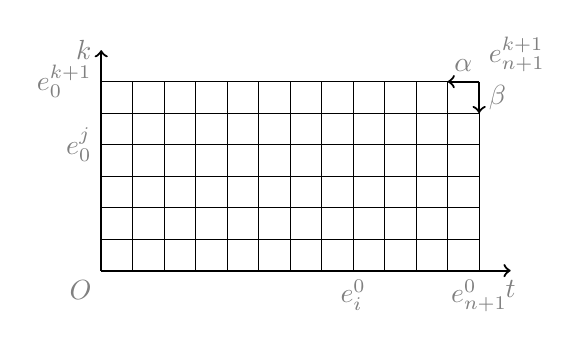
\begin{tikzpicture}[scale=0.4]
    \draw[thick,->] (0, 0) -- (13, 0); \draw[thick,->] (0, 0) -- (0,7); \draw[gray] (0,0) node[anchor=north east] {$O$};
    \draw[gray] (0,7) node[anchor=east] {$k$}; \draw[gray] (13,0) node[anchor=north] {$t$}; \draw[gray] (0,4)
    node[anchor=east] {$e_{0}^{j}$}; \draw[gray] (0,6) node[anchor=east] {$e_{0}^{k+1}$}; \draw[gray] (8,0)
    node[anchor=north] {$e_{i}^{0}$}; \draw[gray] (12,0) node[anchor=north] {$e_{n+1}^{0}$}; \draw[gray] (12,6)
    node[anchor=south west] {$e_{n+1}^{k+1}$}; \foreach \y in {1,2,3,4,5,6} \draw (0,\y) -- (12,\y); \foreach \x in
    {1,2,3,4,5,6,7,8,9,10,11,12} \draw (\x,0) -- (\x,6); \draw[thick,->] (12,6) -- (12, 5); \draw[thick,->] (12,6) --
    (11, 6); \draw[gray] (11.5,6) node[anchor=south] {$\alpha$}; \draw[gray] (12,5.5) node[anchor=west] {$\beta$};
  \end{tikzpicture}
  \caption{误差关系 $e_{n+1}^{k+1}=\alpha e_{n}^{k+1} + \beta e_{n+1}^{k}$}
  \label{fig:error}
\end{figure}

这里选取一个作为例子来说明.想要将 $e_{n+1}^{k+1}$ 移动到 $e_{i}^{0}$, 需要向西移动 $n+1-i$ 步,向南移动 $k+1$ 步.每向西移动一步需要乘以因子 $\alpha$, 每向南移动一步需要乘以因子 $\beta$. 所有可能的路径数为 $\binom{k+n+2-i}{k+1}$. 所有有 $\beta^{k+1} \binom{k+n+2-i}{k+1} \alpha^{n+1-i}e_{i}^{0}$. 类似地,为了移动到 $e_{0}^{j}$, 有 $\alpha^{n+1} \binom{n+k+2-j}{n+1} \beta^{k+1-j}e_{0}^{j}$. 把这些结果加起来,就证明了该结论.

从引理 \ref{lem:error} 可以看出,能够得到一个波形松弛方法误差的精确公式.对于波形松弛方法来说,所有的 $e_{0}^{j}$ 都为零.所以能够得到隐式欧拉波形松弛方法上面的误差结果.

证毕.

\begin{theorem}
\emph{隐式欧拉波形松弛方法的误差为
\begin{equation*}
    e_{n+1}^{k+1}=\beta^{k+1} \sum_{i=1}^{n+1} \binom{k+n+2-i}{k+1} \alpha^{n+1-i}e_{i}^{0},
  \end{equation*}
  式中 $e_{n}^{k}=y_{n}^{k}-y_{n}$, $\displaystyle{\alpha = \frac{1}{1+\Delta t m}}$, 和
  $\displaystyle{\beta = \frac{\Delta t n}{1+\Delta t m}}$.}
\end{theorem}

{\textbf{证明}} 因为所有的 $e_{0}^{j}$ 都为零,该结果可以由引理 \ref{lem:error} 自然得到.

证毕.

\begin{theorem}
  \emph{隐式欧拉波形松弛方法的误差可以用如下式子来控制
  \begin{equation*}
    \| e_{n+1}^{k+1} \| \le \frac{\beta^{k+1} e}{(1-\alpha)^{k+2}},
  \end{equation*}
  式中 $e=\max\limits_{1\le i \le n+1} \|e_{i}^{0}\|$.}
\end{theorem}

{\textbf{证明}} 由下面的几何级数公式
  \begin{equation*}
    \frac{1}{(1-\alpha)^{k+1}}=\sum_{n=0}^{\infty}\binom{k+n}{n}\alpha^n,
  \end{equation*}
  能够得到,如果取 $e=\max\limits_{1\le i \le n+1} \|e_{i}^{0}\|$, 就有
  \begin{equation*}
    \| e_{n+1}^{k+1} \| \le \frac{\beta^{k+1} e}{(1-\alpha)^{k+2}}.
  \end{equation*}

证毕.

从这个定理可以看到,随着 $\beta/(1-\alpha)$ 的减小,误差也在减小.注意到
$\alpha = 1/(1+\Delta t m)$ 和 $\beta = (\Delta t n)/(1+\Delta t m)$, 有
$\beta/(1-\alpha)=n/m$. 事实也是如此,因为当 $n=0$ 时,就是所收敛到的离散格式.

%\subsection{窗口加速技术}
%\esubsection{Windowing Accelerating Technique}
窗口加速技术是由 \cite{zhang1996note} 提出,并在 \cite{jiang2006windowing} 中详细分析的.窗口的长度需要根据所能容忍的误差来决定.取定窗口长度之后,就可以挨个窗口逐次求解了.窗口技术具有天然的可并行性,如图 \ref{fig:para1} 所示.

\begin{figure}[h]
  \centering
  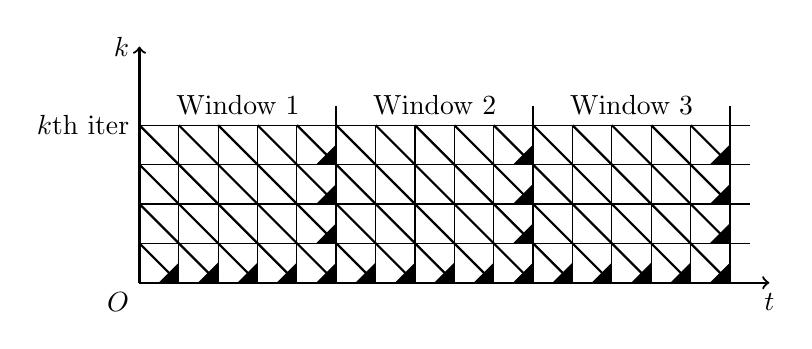
\begin{tikzpicture}[scale=0.5]
    \draw[thick,->] (0, 0) -- (16, 0); \draw[thick,->] (0, 0) -- (0,6); \draw[thick] (0,0) node[anchor=north east] {$O$};
    \draw[thick] (0,6) node[anchor=east] {$k$}; \draw[thick] (16,0) node[anchor=north] {$t$}; \foreach \y in {1,2,3,4}
    \draw (0,\y) -- (15.5,\y); \foreach \x in {1,2,3,4,5,6,7,8,9,10,11,12,13,14,15} \draw (\x,0) -- (\x,4); \draw[thick]
    (5,0) -- (5, 4.5); \draw[thick] (10,0) -- (10, 4.5); \draw[thick] (15,0) -- (15, 4.5); \draw[thick] (2.5,4)
    node[anchor=south] {Window 1}; \draw[thick] (7.5,4) node[anchor=south] {Window 2}; \draw[thick] (12.5,4)
    node[anchor=south] {Window 3}; \draw[thick] (0,4) node[anchor=east] {$k$th iter}; \foreach \z in {0,5,10}{
      \draw[thick,->,-triangle 90] (\z+0,1) -- (\z+1,0); \draw[thick,->,-triangle 90] (\z+0,2) -- (\z+2,0);
      \draw[thick,->,-triangle 90] (\z+0,3) -- (\z+3,0); \draw[thick,->,-triangle 90] (\z+0,4) -- (\z+4,0);
      \draw[thick,->,-triangle 90] (\z+1,4) -- (\z+5,0); \draw[thick,->,-triangle 90] (\z+2,4) -- (\z+5,1);
      \draw[thick,->,-triangle 90] (\z+3,4) -- (\z+5,2); \draw[thick,->,-triangle 90] (\z+4,4) -- (\z+5,3); }
  \end{tikzpicture}
  \caption{窗口技术及其并行策略}
  \label{fig:para1}
\end{figure}

在图 \ref{fig:para1} 中可以看到,窗口之间的技术是串行的,但是,在每个``箭头''上,是可以并行求解的.如果记迭代次数为 $k$, 记每个窗口的时间节点数为 $N$, 那么,需要 $k+N-1$ 步并行的计算.如果串行求解,需要 $Nk$ 步的计算时间.因此,理论的加速比为 $(Nk)/(k+N-1)$.

此外,窗口大小可以由以下公式得到 \cite{jiang2006windowing}
\begin{equation*}
  T_\epsilon=\max\Bigg\{t:\sqrt[k_s]{\int_a^te^{(t-s)L_1}\frac{(t-s)^{k_s-1}}{(k_s-1)!}\,\mathrm{d}s}\le \varepsilon/L_2,\quad t>a\Bigg\},
\end{equation*}
式中 $L_1$ 和 $L_2$ 是由分裂函数所产生的常数, $k_s$ 是每个窗口最大的迭代次数, $a$ 是每个窗口的初始时刻, $\varepsilon$ 是所能容许的误差.

由 \cite{jiang2006windowing} 可知,窗口大小可以取为等间距的,这对于辛方法来说是有利的一个方面,因为取等时间步长是保证长时间计算结果稳定的一个必要条件 \cite{hairer2006geometric}. 这一点是由半群理论所得到的.

\section{流形上基于波形松弛的李群方法}\label{sec:04wrmani}
\esection{Lie Group Method Based on the WR Method on Manifolds}

在这一节里,将介绍适用于一些特定流形上计算的数值方法.该类方法利用了在流形上的作用的李群结构,和其相应的线性空间,即李代数,以及指数映射.

首先考虑这样一类矩阵方程
\begin{equation*}
	y'=A(t)y,\quad t\geq 0,\quad y(0)=y_0,
\end{equation*}
式中 $y_0\in \mathbb{R}^n,\forall t \geq 0,$ $A(t)$ 是一个 $n\times n$ 矩阵.

对于 $n=1$ 的情况,该方程的解可以直接积分得到
\begin{equation*}
	y(t)=e^{\int_0^ta(\xi)d\xi}y_0.
\end{equation*}

然而,对于 $n>1$ 的情况,上面形式的解就不再是方程的解了,只有在满足可交换条件时才能成立.

对于数值解法,正如前面所陈述,对于一个流形上的解,数值结果会远离该流形,导致数值结果不满足理论结果,这并不是我们想要的.因此,有必要重新考虑利用李群的理论,将数值结果限制在该流形上.

在本节,要考虑的是这样一类李群方程
\begin{equation*}
	Y'=A(t,Y)Y,\quad t\geq 0,\quad Y(0)=Y_0,
\end{equation*}
式中 $Y_0\in G $, $A:\mathbb{R}^+\times G\to \mathfrak{g}$, 它的解满足
\begin{equation*}
	Y(t)\in G,\quad t\geq 0.
\end{equation*}

对于这类方程,有几个经典的例子.
\begin{description}
	\item[(1) 正交矩阵流] 满足如下条件的微分方程被称作正交流
	\begin{equation*}
		Y'=A(t,Y)Y,\quad t\geq 0,\quad Y(0)=Y_0\in O(N),
	\end{equation*}
	式中 $A:\mathbb{R}^+\times O(N)\to \mathfrak{so}(N)$. 可以知道对于任意的 $t\geq 0$, 该方程的解 $Y(t)$ 是一个正交矩阵.
	\item[(2) 等谱矩阵流] 满足如下条件的微分方程被称作等谱流
	\begin{equation*}
		Y'=B(t,Y)Y-YB(t,Y),\quad t\geq 0,\quad Y(0)=Y_0\in S_N,
	\end{equation*}
	式中 $B:\mathbb{R}^+\times S_N\to \mathfrak{so}(N)$. 可以知道,该方程的解析解 $Y(t)$ 的特征值随时间保持不变.
\end{description}

\subsection{流形上的李群方法}
\esubsection{Lie Group Method on Manifolds}
这一节,从矩阵李群的概念入手,逐步得到求解流形上微分方程的 Crouch-Grossman 方法和 RK-MK 方法.

\subsubsection{矩阵李群基本概念}
\esubsubsection{Introduction to Matrix Lie Groups}

首先,要对矩阵李群进行讨论.
\begin{definition}
	\emph{一个实数的矩阵李群,是一个光滑的子集 $\mathcal{G}\subseteq \mathbb{R}^{n\times n}$, 在矩阵乘积和矩阵求逆下封闭.记 $I\in \mathcal{G}$ 为单位矩阵.}
\end{definition}

李群的李代数是李群在单位元上的切空间,因此有
\begin{definition}
	\emph{李群 $\mathcal{G}$ 的李代数 $\mathfrak{g}$ 是一个线性子空间 $\mathfrak{g}\subseteq \mathbb{R}^{n\times n}$ 包含了如下形式的所有矩阵
	\begin{equation*}
		\mathfrak{g} = \left\lbrace A \in \mathbb{R}^{n\times n}:A=\left.\frac{d\rho(s)}{ds}\right|_{s=0}\right\rbrace,
	\end{equation*}
	式中 $\rho(s)\in \mathcal{G}$ 是一个光滑曲线,满足 $\rho(0)=I$. 该空间 $\mathfrak{g}$ 在矩阵乘积,标量相乘和矩阵交换子
	\begin{equation*}
		[A,B]=AB-BA,
	\end{equation*}
	下封闭.}
\end{definition}

有了矩阵李群和李代数,就可以定义在矩阵李群上的微分方程.
\begin{definition}
	\emph{在矩阵李群上的微分方程具有如下的形式
	\begin{equation*}
		Y'=A(t,Y)Y,\quad t\geq 0,\quad Y(0)\in \mathcal{G},
	\end{equation*}
	式中 $A:\mathbb{R}\times \mathcal{G}\to \mathfrak{g}$, 并且 $AY$ 就是 $A\in \mathfrak{g}$ 和 $Y\in \mathcal{G}$ 之间的矩阵乘积.}
\end{definition}

对于指数映射,它的形式和指数函数的定义类似.
\begin{definition}
	\emph{矩阵李代数到李群的指数映射 $\mbox{expm}:\mathfrak{g}\to\mathcal{G}$ 定义为
	\begin{equation*}
		\mbox{expm}(A)=\sum_{j=0}^{\infty}\frac{A^j}{j!}.
	\end{equation*}}
\end{definition}

注意到 $\mbox{expm}(O)=I$, 并且对于充分靠近 $O\in \mathfrak{g}$ 的 $A$, 都有一个光滑的逆,记作 $logm:\mathcal{G}\to\mathfrak{g}$.

\begin{definition}
	\emph{矩阵的伴随表示 $Ad$ 和它的导数 $ad$ 有如下定义
	\begin{equation*}
		Ad_P(A)=PAP^{-1},
	\end{equation*}
	\begin{equation*}
		ad_A(B)=AB-BA=[A,B].
	\end{equation*}}
\end{definition}

\begin{definition}
	\emph{指数映射的微分是指数映射的右平凡化切向量,即如下的函数 $dexp:\mathfrak{g}\times \mathfrak{g}\to \mathfrak{g}$, 满足
	\begin{equation*}
		\frac{d}{dt}exp(A(t))=dexp_{A(t)}(A'(t))exp(A(t)).
	\end{equation*}}
\end{definition}

事实上,对于固定的 $A(t)$, 可以看出来 $Ad_A,ad_A,dexp_A$ 都是线性映射.因此,在 $\mathfrak{g}$ 上都可以看作是矩阵.这里的 $dexp_A$ 是一个解析函数
\begin{equation*}
	dexp_A=\frac{\mbox{expm}(ad_A)-I}{ad_A}.
\end{equation*}

该函数可以用指数函数展开
\begin{equation*}
	\begin{aligned}
		dexp_A(C)&=C+\frac{1}{2!}[A,C]+\frac{1}{3!}[A,[A,C]]+\frac{1}{4!}[A,[A,[A,C]]]+\cdots\\
		&=\sum_{j=0}^{\infty}\frac{1}{(j+1)!}ad^j_AC.
	\end{aligned}
\end{equation*}

这里,更需要的是该函数的逆
\begin{equation*}
	dexp_A^{-1}=\frac{ad_A}{\mbox{expm}(ad_A)-I}.
\end{equation*}

对其逆的展开,需要考虑函数
\begin{equation*}
	\frac{x}{e^x-1}=1-\frac{1}{2}x+\frac{1}{12}x^2-\frac{1}{720}x^4+\cdots=\sum_{j=0}^{\infty}\frac{B_j}{j!}x^j,
\end{equation*}
式中 $B_j$ 是伯努利数.该数列在解析数论的黎曼猜想里有着重要的作用.因此,有如下展开
\begin{equation*}
	dexp_A^{-1}(C)=C-\frac{1}{2}[A,C]+\frac{1}{12}[A,[A,C]]+\cdots=\sum_{j=0}^{\infty}\frac{B_j}{j!}ad^j_AC.
\end{equation*}

接下来说明该函数展开的作用,首先给出如下定义
\begin{definition}
	\emph{给定一个函数 $\psi:\mathfrak{g}\to\mathcal{G}$, 其右平凡化切向量被定义为 $d\psi:\mathfrak{g} \times \mathfrak{g} \to \mathfrak{g}$ 满足
	\begin{equation*}
		\frac{d}{dt}\psi(A(t))=d\psi_{A(t)}(A'(t))\psi(A(t)).
	\end{equation*}}
\end{definition}

然后通过 $dexp^{-1}$ 来求得 BCH 公式.定义一个函数 $bch:\mathfrak{g} \times \mathfrak{g} \to \mathfrak{g}$ 满足
\begin{equation*}
	\mbox{expm}(bch(A,B))=\mbox{expm}(A)\mbox{expm}(B).
\end{equation*}

为了计算 $C=bch(A,B)$, 把它写成微分方程.令 $C(t)=bch(tA,B)$. 显然有 $C(0)=B$, 用此来计算 $C(t)$. 把式
\begin{equation*}
	\mbox{expm}(C(t))=\mbox{expm}(tA)\mbox{expm}(B)
\end{equation*}
对 $t$ 求微分,有
\begin{equation*}
	dexp_{C(t)}(C'(t))exp(C(t))=dexp_{tA}exp(tA)exp(B)=A~exp(C(t)),
\end{equation*}
因此有
\begin{equation*}
	C'(t)=dexp_{C(t)}^{-1}(A).
\end{equation*}

于是,有如下定理
\begin{theorem}
	\emph{函数 $C=bch(A,B)$ 可以由如下的微分方程来计算
	\begin{equation*}
		C'(t)=dexp_{C(t)}^{-1}(A),\quad 0\leq t\leq 1,\quad C(0)=B,
	\end{equation*}
	式中 $C(1)=bch(A,B)$.}
\end{theorem}

可以看到,该微分方程右端的式子,可以由前面的展开式得到近似,这对于设计求解李群方程的数值方法有着重要的作用.

关于流形上的李群方法,通常来说有两种手段,一种是 Crouch-Grossman 方法 \cite{crouch1993numerical,klein2013numerical,munthe2013onpost,sonneville2014geome,bras2011anonlinear,kroshko2011integrating} ,另一种是 RK-MK \cite{arieh2005liegroup} 方法.

\subsubsection{Crouch-Grossman 方法}
\esubsubsection{The Crouch-Grossman Methods}
Crouch-Grossman(CG) 方法可以说是李群数值方法的带头人,该方法是较早提出的流形上的优秀的数值方法.有趣的是,该方法最初的应用是机器人和控制理论.

从本质上讲,该算法是将 Runge-Kutta 方法作用到李群方程上的一个有效尝试.该方法通过不断地冻结和融化系数,保证了解的流在流形的配置空间上.

该方法的基本思想是,先沿着一个方向走一小步,然后利用指数映射,将结果投射到流形上.每次都这样,直到完成一步 Runge-Kutta 的步骤.因此,经过一个 CG 方法迭代,数值结果还在流形上.尽管该结果也会带来误差,但是不会脱离流形.

对比 Runge-Kutta 法, Crouch-Grossman 方法的基本形式是
\begin{equation*}
\left.\begin{aligned}
		X_k&=e^{ha_{k,k-1}F_{k-1}}e^{ha_{k,k-2}F_{k-2}}\cdots e^{ha_{k,1}F_{1}}Y_n\\
		F_k&=A(t_n+c_kh,X_k)\\
		Y_{n+1}&=e^{hb_{\nu}F_{\nu}}e^{hb_{\nu-1}F_{\nu-1}}\cdots e^{hb_{1}F_{1}}Y_n
	\end{aligned}\right\rbrace\quad k=1,2,\ldots,\nu.
\end{equation*}

可以看出来,该方法是一个显式方法.一个早先的三步三阶方法 \cite{crouch1993numerical} 是
\begin{equation*}
	\begin{aligned}
		X_1&=Y_n,\\
		F_1&=A(t_n,X_1),\\
		X_2&=e^{\frac{3}{4}hF_1}Y_n,\\
		F_2&=A(t_n+\frac{3}{4}h,X_2),\\
		X_3&=e^{\frac{17}{108}hF_2}e^{\frac{119}{216}hF_1}Y_n,\\
		F_2&=A(t_n+\frac{17}{24}h,X_3),\\
		Y_{n+1}&=e^{\frac{13}{51}hF_3}e^{-\frac{2}{3}hF_2}e^{\frac{24}{17}hF_1}Y_n.
	\end{aligned}
\end{equation*}

后来,有人将其推广到隐式方法,隐式方法需要将上面的 $X_k$ 变成
\begin{equation*}
	X_k=e^{ha_{k,\nu}F_{\nu}}e^{ha_{k,\nu-1}F_{\nu-1}}\cdots e^{ha_{k,1}F_{1}}Y_n,\quad k=1,2,\ldots,\nu.
\end{equation*}

隐式方法的缺点是求解流形上的隐式问题更加复杂.

\subsubsection{RK-MK 方法}
\esubsubsection{The Runge-Kutta-Munthe-Kaas Methods}
相比之下, RK-MK 方法更加实用.这些方法又叫做 RK-MK 类方法,方法及其理论由陆续的几篇文章 \cite{mk1996lie,mk1997numerical,mk1998runge,mk1999high} 建立起来.该方法和 CG 方法类似,利用了指数映射.不同的是, CG 方法每走一小步都要求落回到流形上, RK-MK 方法先在李代数这个线性空间上进行计算,最后用指数映射保证这一步的计算结果在流形上.

该方法建立在如下的理论上.
\begin{theorem}
	\emph{对于很小的 $t\geq 0$, 李群方法的解有如下的形式
	\begin{equation*}
		Y(t)=\mbox{expm}(\Theta(t))Y_0,
	\end{equation*}
	式中 $\Theta \in \mathfrak{g}$ 满足微分方程
	\begin{equation*}
		\Theta'(t)=dexp_{\Theta(t)}^{-1}(A(t,Y))\quad \Theta(0)=O,
	\end{equation*}
	这里的 $dexp$ 为指数映射的微分.}
\end{theorem}

该定理告诉我们,如果能够求得 $\Theta(t)$, 就可以代入这个解,求得李群方程的解.首先,给出 Butcher 表
\begin{center}
  \begin{tabular}{c|cccc}
    $c_1$&$a_{11}$&$a_{12}$&$\cdots$&$a_{1\nu}$\\
    $c_2$&$a_{21}$&$a_{22}$&$\cdots$&$a_{2\nu}$\\
    $\vdots$&$\vdots$&$\vdots$&$\ddots$&$\vdots$\\
    $c_{\nu}$&$a_{\nu 1}$&$a_{\nu 2}$&$\cdots$&$a_{\nu \nu}$\\
    \hline
         &$b_{1}$&$b_{2}$&$\cdots$&$b_{\nu}$
  \end{tabular}
\end{center}
式中这里的常数,为 Runge-Kutta 法里的常数. RK-MK 法利用了 RK 法的基本思想,结合了李群指数映射的特性,具有比较好的数值效果.
\begin{equation*}
	\begin{aligned}
		&\left.\begin{aligned}
		\Theta_k&=\sum_{l=1}^{\nu}a_{k,l}F_l,\\
		A_k&=hA(t_n+c_kh,\mbox{expm}(\Theta_k)Y_n),\\
		F_k&=dexp_{\Theta_k}^{-1}(A_k),
	\end{aligned}\right\rbrace \quad k=1,2,\ldots,\nu\\
		&\begin{aligned}
		\Theta&=\sum_{l=1}^{\nu}b_lF_l,\\
		Y_{n+1}&=\mbox{expm}(\Theta)Y_n.
	\end{aligned}
	\end{aligned}
\end{equation*}

可以看到,这里的 $dexp_{\Theta_k}^{-1}(A_k)$ 可以用前面的展开式进行计算,为了简化,这里只需展开几项进行计算.

需要注意的是,为了计算 $ad^j_AC$, 需要如下递推公式得到
\begin{equation*}
	ad^0(u)(v)=v,
\end{equation*}
\begin{equation*}
	ad^n(u)(v)=ad(u)(ad^{n-1}(u)(v))=[u,[u,[\cdots,[u,v]]]],\quad \forall n \geq 1.
\end{equation*}

展开的项数也有要求,可以根据如下定理.
\begin{theorem}
	\emph{若 Runge-Kutta 方法有 $p$ 阶, $dexp^{-1}$ 展开式中取到 $q$ 项,且 $q\geq p-1$, 则相应的 RK-MK 方法为 $p$ 阶的.}
\end{theorem}

这里给出一个 RK-MK 方法的例子.对于如下的 Butcher 表
\begin{center}
  \begin{tabular}{c|cccc}
    $0$&&&&\\
    $\frac{1}{2}$&$\frac{1}{2}$&&&\\
    $\frac{1}{2}$&$0$&$\frac{1}{2}$&&\\
    $1$&$0$&$0$&$1$&\\
    \hline
         &$\frac{1}{6}$&$\frac{1}{3}$&$\frac{1}{3}$&$\frac{1}{6}$
  \end{tabular}
\end{center}

则对应的 $4$ 阶精度的 RK-MK 法如下
\begin{equation*}
	\begin{aligned}
		&\psi_1=0,\\
		&A_1=hA(t_n,y_n),\\
		&K_1=A_1,\\
		&\psi_2=\frac{1}{2}K_1,\\
		&A_2=hA(t_n+\frac{1}{2}h,e^{\psi_2}y_n),\\
		&K_2=A_2-\frac{1}{2}[\psi_2,A_2]+\frac{1}{12}[\psi_2,[\psi_2,A_2]],\\
		&\psi_3=\frac{1}{2}K_2,\\
		&A_3=hA(t_n+\frac{1}{2}h,e^{\psi_3}y_n),\\
		&K_3=A_3-\frac{1}{2}[\psi_3,A_3]+\frac{1}{12}[\psi_3,[\psi_3,A_3]],\\
		&\psi_4=K_3,\\
		&A_4=hA(t_n+h,e^{\psi_4}y_n),\\
		&K_4=A_4-\frac{1}{2}[\psi_4,A_4]+\frac{1}{12}[\psi_4,[\psi_4,A_4]],\\
		&y_{n+1}=exp(\frac{1}{6}K_1+\frac{1}{3}K_2+\frac{1}{3}K_3+\frac{1}{6}K_4)y_n.
	\end{aligned}
\end{equation*}

可以看出来,和 CG 方法相比,这种方法减少了指数映射的计算次数,因此就减少了计算量和精度分析的难度.

注意到,上面的方法是显式的,这样的计算是很容易的.但是尽管这样计算具有便利性,该计算却不能具有其他很好的效果,如果一个李群方程不仅要求数值结果在流形上,而且要求该数值方法保持某些结构,可能需要一些隐式方法来求解.这个问题类比于哈密尔顿系统,有一个守恒量,但是目前的方法只能保证结果在流形上,却无法保证在流形上有保结构的结果.

对于上面的不足,对于一些情况,需要隐式的 RK-MK 方法,于是就有了对其的显式改造,即利用波形松弛方法进行改造.

%\section{流形上的波形松弛方法}\label{sec:04wrmani}
%\esection{Waveform Relaxation Methods on Manifolds}

\subsection{主要方法讨论}
\esubsection{Discussions on the Main Method}

在本小节,给出隐式的 RK-MK 方法的一个波形松弛改造,首先回归到 RK-MK 的基本算法上
\begin{equation*}
	\begin{aligned}
		&\left.\begin{aligned}
		\Theta_k&=\sum_{l=1}^{\nu}a_{k,l}F_l,\\
		A_k&=hA(t_n+c_kh,\mbox{expm}(\Theta_k)Y_n),\\
		F_k&=dexp_{\Theta_k}^{-1}(A_k),
	\end{aligned}\right\rbrace \quad k=1,2,\ldots,\nu\\
		&\begin{aligned}
		\Theta&=\sum_{l=1}^{\nu}b_lF_l,\\
		Y_{n+1}&=\mbox{expm}(\Theta)Y_n.
	\end{aligned}
	\end{aligned}
\end{equation*}

这里面最重要的是最后一步的更新
\begin{equation*}
	Y_{n+1}=\mbox{expm}(\Theta)Y_n,
\end{equation*}
此处的 $\Theta$ 为李代数上的更新,指数映射将其拉回流形上.前三项循环的部分主要是为了求解 $F_k$, 可以通过代入得到关于 $F_k$ 的代数方程
\begin{equation*}
	F_k=dexp_{\Theta_k}^{-1}(hA(t_n+c_kh,\mbox{expm}(\sum_{l=1}^{\nu}a_{k,l}F_l)Y_n)).
\end{equation*}

因此,该算法可以写成
\begin{equation*}
	\begin{aligned}
		\Theta_k&=\sum_{l=1}^{\nu}a_{k,l}F_l,\quad k=1,2,\ldots,\nu,\\
		F_k&=dexp_{\Theta_k}^{-1}(hA(t_n+c_kh,\mbox{expm}(\sum_{l=1}^{\nu}a_{k,l}F_l)Y_n)),\quad k=1,2,\ldots,\nu,\\
		Y_{n+1}&=\mbox{expm}(\sum_{l=1}^{\nu}b_lF_l)Y_n.
	\end{aligned}
\end{equation*}

可以看到,隐式的 RK-MK 方法就是先求解 $F_k,k=1,2,\ldots,\nu$ 然后代入最后一个式子.

参考辛 Runge-Kutta 波形松弛方法的形式 \cite{bellen1993use} 来设计这里的算法,主要问题是如何使得格式容易计算
\begin{equation*}
  \left\lbrace
    \begin{aligned}
      Y_{n+1}^{r,(k+1)}&=\eta^{(k+1)}(t_{n})+h\sum_{s=1}^{\nu}a_{rs}F(t_{n+1}^{s},Y_{n+1}^{s,(k+1)},Y_{n+1}^{s,(k)}),\quad r=1,\cdots, \nu, \\
      \eta^{(k+1)}(t_{n+1})&=\eta^{(k+1)}(t_{n})+h\sum_{s=1}^{\nu}b_{s}F(t_{n+1}^{s},Y_{n+1}^{s,(k+1)},Y_{n+1}^{s,(k)}).
    \end{aligned}
  \right.
\end{equation*}

要对其中一步
\begin{equation*}
	F_k=dexp_{\Theta_k}^{-1}(hA(t_n+c_kh,\mbox{expm}(\sum_{l=1}^{\nu}a_{k,l}F_l)Y_n)),\quad k=1,2,\ldots,\nu,
\end{equation*}
进行改造,把它展开即
\begin{equation*}
	\begin{aligned}
		F_1&=dexp_{\Theta_1}^{-1}(hA(t_n+c_1h,\mbox{expm}(\sum_{l=1}^{\nu}a_{1,l}F_l)Y_n)),\\
		F_2&=dexp_{\Theta_2}^{-1}(hA(t_n+c_2h,\mbox{expm}(\sum_{l=1}^{\nu}a_{2,l}F_l)Y_n)),\\
		&\cdots \\
		F_{\nu}&=dexp_{\Theta_{\nu}}^{-1}(hA(t_n+c_{\nu}h,\mbox{expm}(\sum_{l=1}^{\nu}a_{\nu,l}F_l)Y_n)),
	\end{aligned}
\end{equation*}
式中 $\Theta_k=\sum_{l=1}^{\nu}a_{k,l}F_l,\quad k=1,2,\ldots,\nu$.

这里,一方面要考虑上面方程里 $F_k$ 的求解,另一方面要考虑最后的步进公式的设置
\begin{equation*}
	Y_{n+1}=\mbox{expm}(\sum_{l=1}^{\nu}b_lF_l)Y_n.
\end{equation*}

如果采用 Picard 波形松弛格式,该算法可以写成
\begin{equation*}
	\left\lbrace\begin{aligned}
		F_1^{n+1,(k+1)}&=dexp_{\Theta_1^{n+1,(k)}}^{-1}(hA(t_n+c_1h,\mbox{expm}(\sum_{l=1}^{\nu}a_{1,l}F_l^{n+1,(k)})Y_n^{(k)})),\\
		F_2^{n+1,(k+1)}&=dexp_{\Theta_2^{n+1,(k)}}^{-1}(hA(t_n+c_2h,\mbox{expm}(\sum_{l=1}^{\nu}a_{2,l}F_l^{n+1,(k)})Y_n^{(k)})),\\
		\cdots \\
		F_{\nu}^{n+1,(k+1)}&=dexp_{\Theta_{\nu}^{n+1,(k)}}^{-1}(hA(t_n+c_{\nu}h,\mbox{expm}(\sum_{l=1}^{\nu}a_{\nu,l}F_l^{n+1,(k)})Y_n^{(k)})),\\
		Y_{n+1}^{(k+1)}&=\mbox{expm}(\sum_{l=1}^{\nu}b_lF_l^{n+1,(k)})Y_n^{(k)},
	\end{aligned}\right.
\end{equation*}
式中 $\Theta_m^{n+1,(k)} = \sum_{l=1}^{\nu}a_{m,l}F_l^{n+1,(k)}$, $F_l^{n+1,(k)}$ 中的下指标 $l$ 是 Runge-Kutta 的步数, 上指标 $k$ 为波形松弛方法的步数, 上指标 $n+1$ 是时间节点序数.

如果采用 Gauss-Jacobi 波形松弛格式,该算法可以写成
\begin{equation*}
	\left\lbrace\begin{aligned}
		F_1^{n+1,(k+1)}&=dexp_{\Theta_1^{n+1,(k)}}^{-1}(hA(t_n+c_1h,\mbox{expm}(a_{1,1}F_1^{n+1,(k+1)}+\sum_{l=1,l\neq 1}^{\nu}a_{1,l}F_l^{n+1,(k)})Y_n^{(k)})),\\
		F_2^{n+1,(k+1)}&=dexp_{\Theta_2^{n+1,(k)}}^{-1}(hA(t_n+c_2h,\mbox{expm}(a_{2,2}F_2^{n+1,(k+1)}+\sum_{l=1,l\neq 2}^{\nu}a_{2,l}F_l^{n+1,(k)})Y_n^{(k)})),\\
		\cdots \\
		F_{\nu}^{n+1,(k+1)}&=dexp_{\Theta_{\nu}^{n+1,(k)}}^{-1}(hA(t_n+c_{\nu}h,\mbox{expm}(a_{\nu,\nu}F_{\nu}^{n+1,(k+1)}+\sum_{l=1,l\neq \nu}^{\nu}a_{\nu,l}F_l^{n+1,(k)})Y_n^{(k)})),\\
		Y_{n+1}^{(k+1)}&=\mbox{expm}(\sum_{l=1}^{\nu}b_lF_l^{n+1,(k)})Y_n^{(k)},
	\end{aligned}\right.
\end{equation*}
式中 $\Theta_m^{n+1,(k)} = F_{m}^{n+1,(k+1)}+\sum_{l=1,l\neq m}^{\nu}a_{m,l}F_l^{n+1,(k)}$.

如果采用 Gauss-Seidel 波形松弛格式,该算法可以写成
\begin{equation*}
	\left\lbrace\begin{aligned}
		F_1^{n+1,(k+1)}&=dexp_{\Theta_1^{n+1,(k)}}^{-1}(hA(t_n+c_1h,\mbox{expm}(a_{1,1}F_1^{n+1,(k+1)}+\sum_{l=2}^{\nu}a_{1,l}F_l^{n+1,(k)})Y_n^{(k)})),\\
		F_2^{n+1,(k+1)}&=dexp_{\Theta_2^{n+1,(k)}}^{-1}(hA(t_n+c_2h,\mbox{expm}(\sum_{l=1}^{2}a_{2,l}F_l^{n+1,(k+1)}+\sum_{l=3}^{\nu}a_{2,l}F_l^{n+1,(k)})Y_n^{(k)})),\\
		\cdots \\
		F_{\nu}^{n+1,(k+1)}&=dexp_{\Theta_{\nu}^{n+1,(k)}}^{-1}(hA(t_n+c_{\nu}h,\mbox{expm}(\sum_{l=1}^{\nu}a_{\nu,l}F_{l}^{n+1,(k+1)})Y_n^{(k)})),\\
		Y_{n+1}^{(k+1)}&=\mbox{expm}(\sum_{l=1}^{\nu}b_lF_l^{n+1,(k)})Y_n^{(k)},
	\end{aligned}\right.
\end{equation*}
式中 $\Theta_m^{n+1,(k)} = \sum_{l=1}^{m}a_{m,l}F_{l}^{n+1,(k+1)}+\sum_{l=m+1}^{\nu}a_{m,l}F_l^{n+1,(k)}$.

也可以设计比 Gauss-Seidel 格式更简单的格式
\begin{equation*}
	\left\lbrace\begin{aligned}
		F_1^{n+1,(k+1)}&=dexp_{\Theta_1^{n+1,(k)}}^{-1}(hA(t_n+c_1h,\mbox{expm}(\sum_{l=1}^{\nu}a_{1,l}F_l^{n+1,(k)})Y_n^{(k)})),\\
		F_2^{n+1,(k+1)}&=dexp_{\Theta_2^{n+1,(k)}}^{-1}(hA(t_n+c_2h,\mbox{expm}(a_{2,1}F_1^{n+1,(k+1)}+\sum_{l=2}^{\nu}a_{2,l}F_l^{n+1,(k)})Y_n^{(k)})),\\
		\cdots \\
		F_{\nu}^{n+1,(k+1)}&=dexp_{\Theta_{\nu}^{n+1,(k)}}^{-1}(hA(t_n+c_{\nu}h,\mbox{expm}(\sum_{l=1}^{\nu-1}a_{\nu,l}F_{l}^{n+1,(k+1)}+a_{\nu,\nu}F_{\nu}^{n+1,(k)})Y_n^{(k)})),\\
		Y_{n+1}^{(k+1)}&=\mbox{expm}(\sum_{l=1}^{\nu}b_lF_l^{n+1,(k)})Y_n^{(k)},
	\end{aligned}\right.
\end{equation*}
式中 $\Theta_m^{n+1,(k)} = \sum_{l=1}^{m-1}a_{m,l}F_{l}^{n+1,(k+1)}+\sum_{l=m}^{\nu}a_{m,l}F_l^{n+1,(k)}$.

%\subsection{基本算法}
%\esubsection{Algorithm}
为了得到较好的计算格式,和辛波形松弛方法一样,继续引入窗口技术,得到如下含有多重循环的算法 \ref{alg:04sym}.

\begin{algorithm}
\caption{李群方程加窗口的波形松弛方法}
\label{alg:04sym}
\begin{algorithmic}
\STATE 初始化解矩阵
\FOR{$w= 1~\texttt{to} ~n_w$}
    \FOR{$k= 1~\texttt{to} ~n_k$}
        \FOR{$s= 1~\texttt{to} ~n_s$}
             \STATE 计算 $Y_{n+1}^{(k+1)}$.
        \ENDFOR
    \ENDFOR
\ENDFOR
\STATE 保存结果.
\end{algorithmic}
\end{algorithm}
在算法 \ref{alg:04sym} 中, $n_w$, $n_k$ 和 $n_s$ 分别代表``窗口数'',``波形松弛迭代次数''和``每个窗口的区间数''.这里需要注意保存至少两步的中间变量 $F_l^{n+1,(k)}$, 才能保证计算正确.

\section{数值实验}\label{sec:03numerical}
\esection{Numerical Experiments}
在本节,将给出四个数值算例来验证我们的算法分析.首先我们把算法的基本框架列出来,见算法 \ref{alg:sym}.

\begin{algorithm}
\caption{窗口辛波形松弛方法}
\label{alg:sym}
\begin{algorithmic}
\STATE 初始化解矩阵
\FOR{$w= 1~\texttt{to} ~n_w$}
    \FOR{$k= 1~\texttt{to} ~n_k$}
        \FOR{$s= 1~\texttt{to} ~n_s$}
             \STATE 用 \eqref{eq:discrete} 计算 $z_{n+1}^{k+1}$.
        \ENDFOR
    \ENDFOR
\ENDFOR
\STATE 保存结果.
\end{algorithmic}
\end{algorithm}

在算法 \ref{alg:sym} 中, $n_w$, $n_k$ 和 $n_s$ 分别代表``窗口数'',``波形松弛迭代次数''和``每个窗口的区间数''. 公式 \eqref{eq:discrete} 可以根据算法的不同进行替换.为了加速算法,可以进行并行计算.该算法在 $t-k$ 平面上的一个图示为图 \ref{fig:para2}.

\begin{figure}[h]
  \centering
  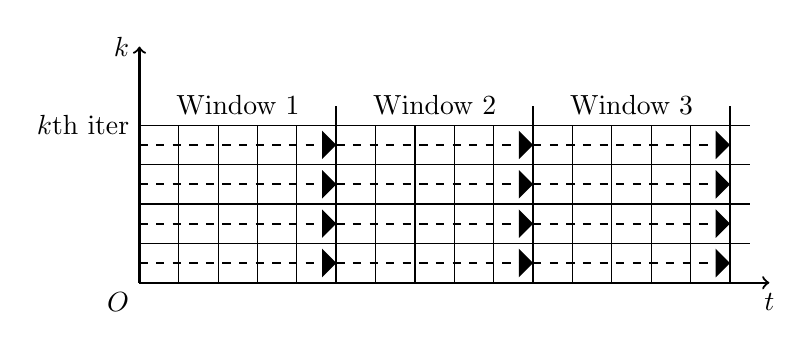
\begin{tikzpicture}[scale=0.5]
    \draw[thick,->] (0, 0) -- (16, 0); \draw[thick,->] (0, 0) -- (0,6); \draw[thick] (0,0) node[anchor=north east] {$O$};
    \draw[thick] (0,6) node[anchor=east] {$k$}; \draw[thick] (16,0) node[anchor=north] {$t$}; \foreach \y in {1,2,3,4}
    \draw (0,\y) -- (15.5,\y); \foreach \x in {1,2,3,4,5,6,7,8,9,10,11,12,13,14,15} \draw (\x,0) -- (\x,4); \draw[thick]
    (5,0) -- (5, 4.5); \draw[thick] (10,0) -- (10, 4.5); \draw[thick] (15,0) -- (15, 4.5); \draw[thick] (2.5,4)
    node[anchor=south] {Window 1}; \draw[thick] (7.5,4) node[anchor=south] {Window 2}; \draw[thick] (12.5,4)
    node[anchor=south] {Window 3}; \draw[thick] (0,4) node[anchor=east] {$k$th iter};
    	\foreach \y in {0,5,10}{
		\foreach \z in {0,1,2,3}{
			\draw[dashed,thick,->,-triangle 90] (\y+0,\z+0.5) -- (\y+5,\z+0.5);
		}
	}
  \end{tikzpicture}
  \caption{算法 \ref{alg:sym} 的图示}
  \label{fig:para2}
\end{figure}

\subsection*{例 1}
考虑如下的一维 sin-Gordon 方程
\begin{equation}\label{eq:singordon}
  \left \{ \begin{array}{l}
      \displaystyle \frac{d^2 u }{d t^2} + u = -\sin u, \quad 0<t \leq t_{\text{end}},\\
      u(x, 0) = 0, \; u_t (x, 0) = 1.
    \end{array} \right.
\end{equation}
令 $q = u$ 和 $\dot{q} = p$, 可以化成如下的哈密尔顿系统
\begin{equation}\label{eq:singordonH}
  \left \{ \begin{array}{l}
      \displaystyle \frac{d q }{d t} = p,\\
      \displaystyle \frac{d p }{d t} = -q - \sin q,
    \end{array} \right.
\end{equation}
初值条件为 $q(0)=0$, $p(0)=1$, 哈密尔顿函数为
\begin{equation*}
  H(q,p) = \frac{p^2}{2} + \frac{q^2}{2} - \cos q.
\end{equation*}

首先考虑辛欧拉波形松弛方法~\eqref{eq:schemejacobi}. 取 $t_{\text{end}} = 200$, 步长为 $h = 1/100$, 波形松弛迭代次数为 $k=15$. 对于窗口加速方法,取每个时间窗口为 $1$. 图 \ref{fig:ex1seucom} 展示了辛欧拉波形松弛方法无窗口加速(左图)和有窗口加速(右图)的比较.发现经典的波形松弛方法需要更多的步数才能收敛.

\begin{figure}[h!]
  \centering
  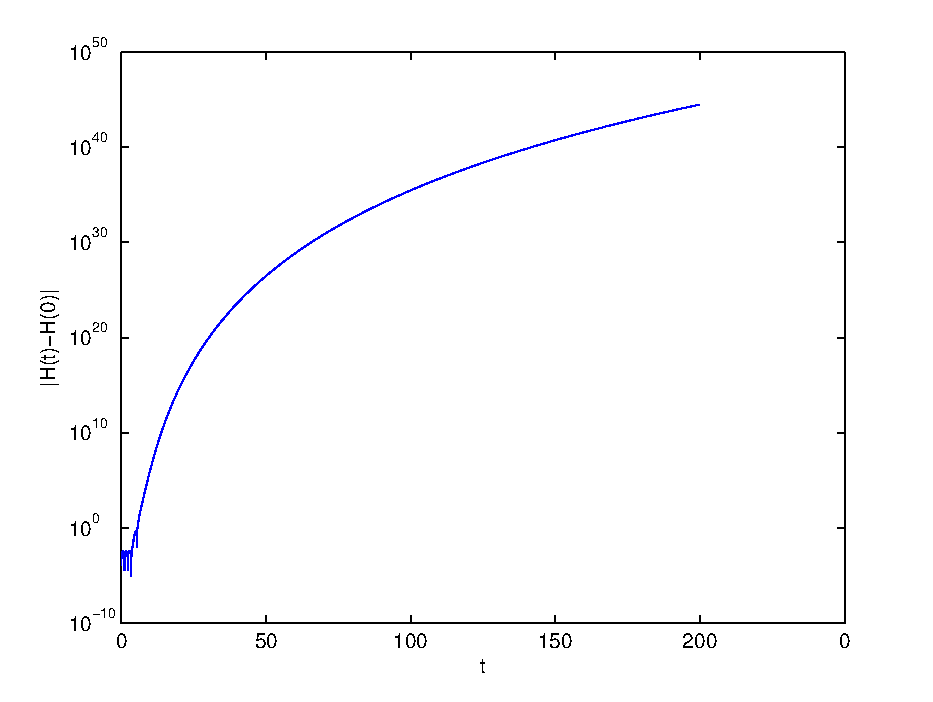
\includegraphics[width=0.45\textwidth]{03/Fig3-1.pdf}
  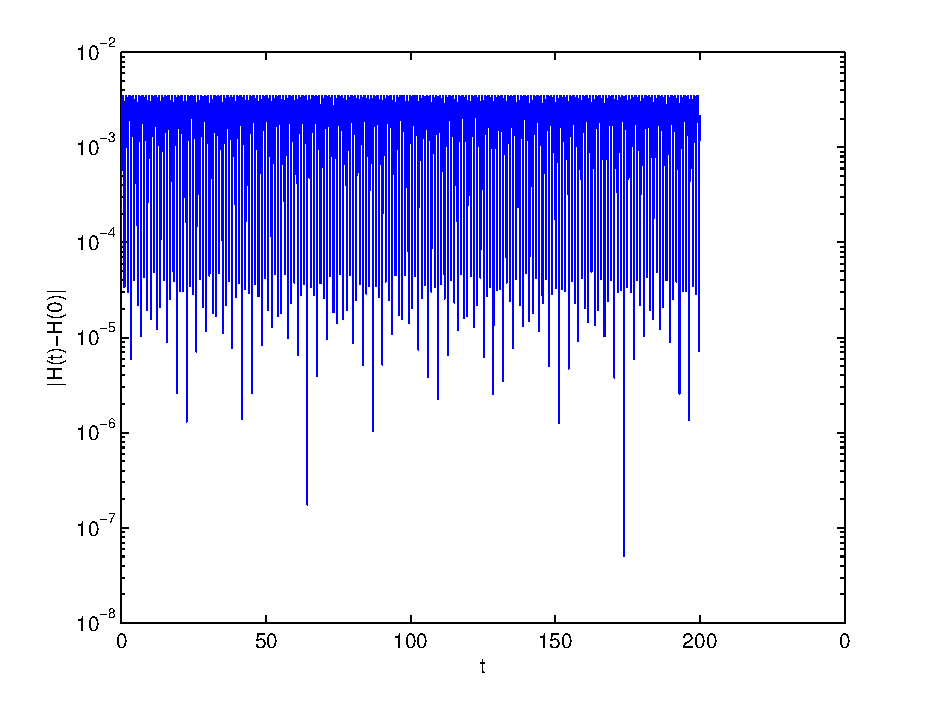
\includegraphics[width=0.45\textwidth]{03/Fig3-2.pdf}
  \caption{sin-Gordon 方程 \eqref{eq:singordon} 辛欧拉波形松弛方法无窗口加速(左图)和有窗口加速(右图)的比较}
  \label{fig:ex1seucom}
\end{figure}

其次,考虑辛 Runge-Kutta 波形松弛方法~\eqref{eq:schemerkjacobi}. 取 $t_{\text{end}} = 200$, 步长为 $h = 1/100$, 波形松弛迭代次数为 $k=15$. 对于窗口加速方法,取每个时间窗口为 $1$. 图 \ref{fig:ex1srkcom} 展示了辛 Runge-Kutta 波形松弛方法无窗口加速(左图)和有窗口加速(右图)的比较.发现经典的波形松弛方法需要更多的步数才能收敛.在本例中使用了表 \ref{tbl:rk} 中的 Butcher 表,其中 $a = 1.351207$.

\begin{table}[h!]
  \centering
  \caption{三阶 Butcher 表}
  \label{tbl:rk}
  \begin{tabular}{c|ccc}
    $\frac{1}{2}a$ & $\frac{1}{2}a$ & & \\
    $\frac{3}{2}a$ & $a$ &$\frac{1}{2}a$  & \\
    $\frac{1}{2} + a$ & $a$ & $a$ &$\frac{1}{2}-a$\\
    \hline
    & $a$ &$a$ & $1-2a$\\
  \end{tabular}
\end{table}

\begin{figure}[h!]
  \centering
  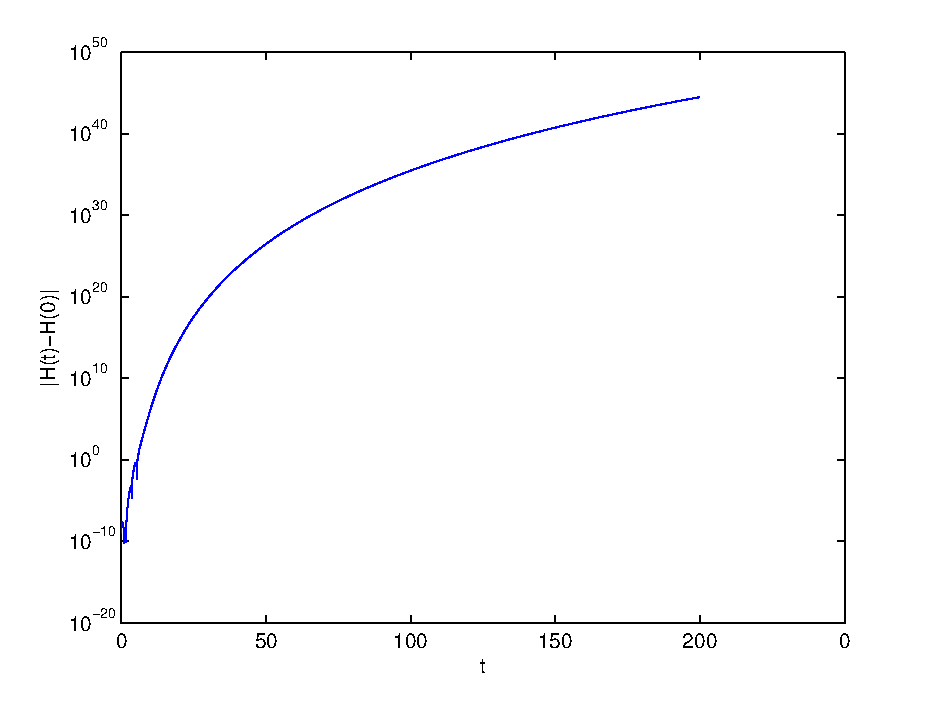
\includegraphics[width=0.45\textwidth]{03/Fig4-1.pdf}
  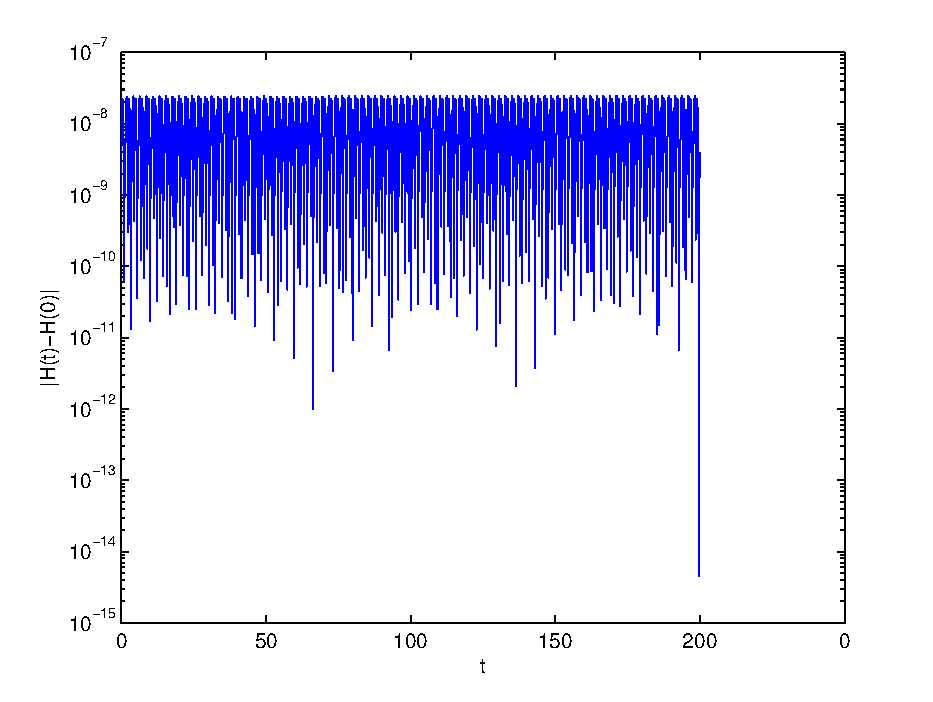
\includegraphics[width=0.45\textwidth]{03/Fig4-2.pdf}
  \caption{sin-Gordon 方程 \eqref{eq:singordon} 辛 Runge-Kutta 波形松弛方法无窗口加速(左图)和有窗口加速(右图)的比较}
  \label{fig:ex1srkcom}
\end{figure}

接下来考虑辛欧拉波形松弛方法和辛 Runge-Kutta 波形松弛方法.取 $t_{\text{end}} = 200$, 步长为 $h = 1/100$, 波形松弛迭代次数为 $k=15$. 对于窗口加速方法,取每个时间窗口为 $1$. 数值结果见表 \ref{tbl:order}. 在此表中辛欧拉波形松弛方法被记作 ``seulerwrwin'',辛 Runge-Kutta 波形松弛方法被记作 ``srkwrwin''.

\begin{table}[h!]
    \begin{center}
    \caption{两种方法随时间步长 $h$ 的变化}
    \label{tbl:order}
    \begin{tabularx}{\linewidth}{XXXXX}
        \toprule[1.5pt]
        h & 4/100 & 2/100 & 1/100 & 1/200\\
        \midrule[1pt]
        seulerwrwin & 0.0143 &0.0071 &0.0035 &0.0017\\
        srkwrwin    & 1.6750e-06 & 1.9805e-07 & 2.4330e-08 & 3.3278e-09\\
        \bottomrule[1.5pt]
    \end{tabularx}
    \end{center}
  \end{table}

最后,考虑该算法的收敛性质,图 \ref{fig:ex1err} 展示了辛欧拉波形松弛方法和辛 Runge-Kutta 波形松弛方法在无窗口的情形下的收敛性质.这里,取 $t_{end} =\textbf{1}$, 步长为 $h=1/100$. 全局最大误差为 $0.0035$.

图 \ref{fig:ex1winerr} 展示了辛欧拉波形松弛方法和辛 Runge-Kutta 波形松弛方法在有窗口的情形下的收敛性质.这里,取 $t_{end} =\textbf{1}$, 步长为 $h=1/100$, 每个时间窗口为 $1$. 全局最大误差为 $2.4330e-08$.

\begin{figure}[h!]
  \centering
  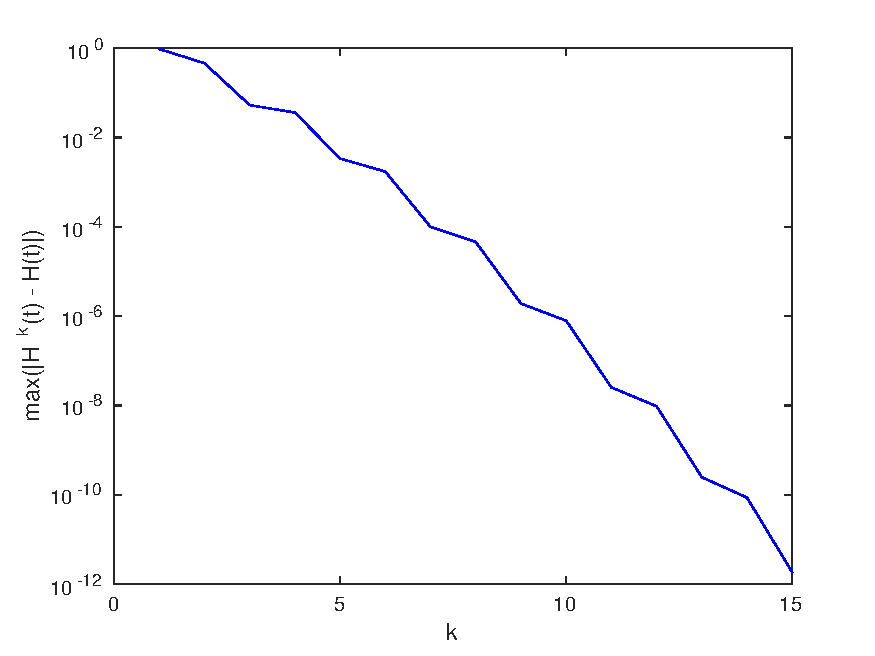
\includegraphics[width=0.45\textwidth]{03/Fig5-1.pdf}
  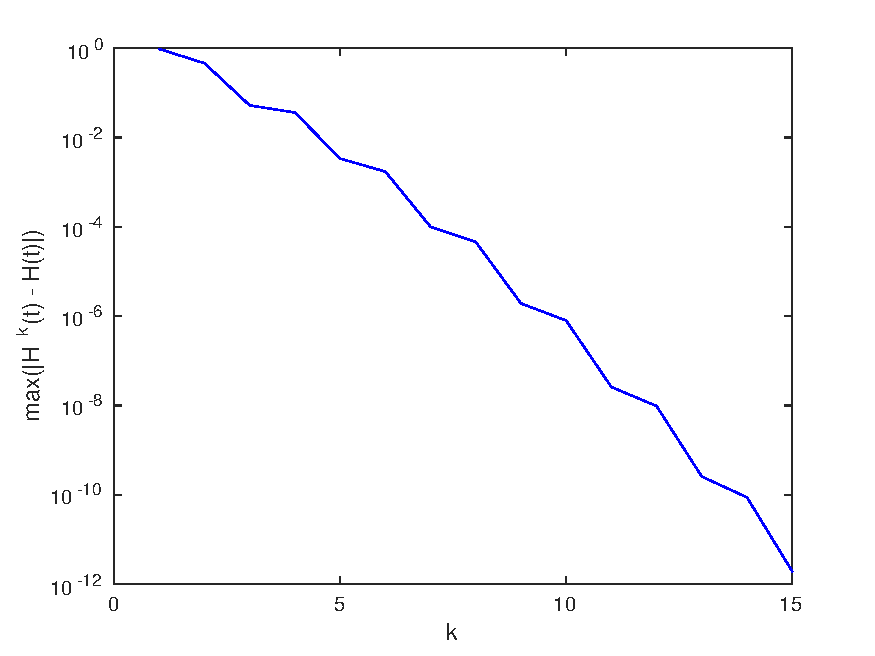
\includegraphics[width=0.45\textwidth]{03/Fig5-2.pdf}
  \caption{sin-Gordon 方程 \eqref{eq:singordon} 辛欧拉波形松弛方法(左图)和辛 Runge-Kutta 波形松弛方法(右图)在无窗口的情形下的比较}
  \label{fig:ex1err}
\end{figure}

\begin{figure}[h!]
  \centering
  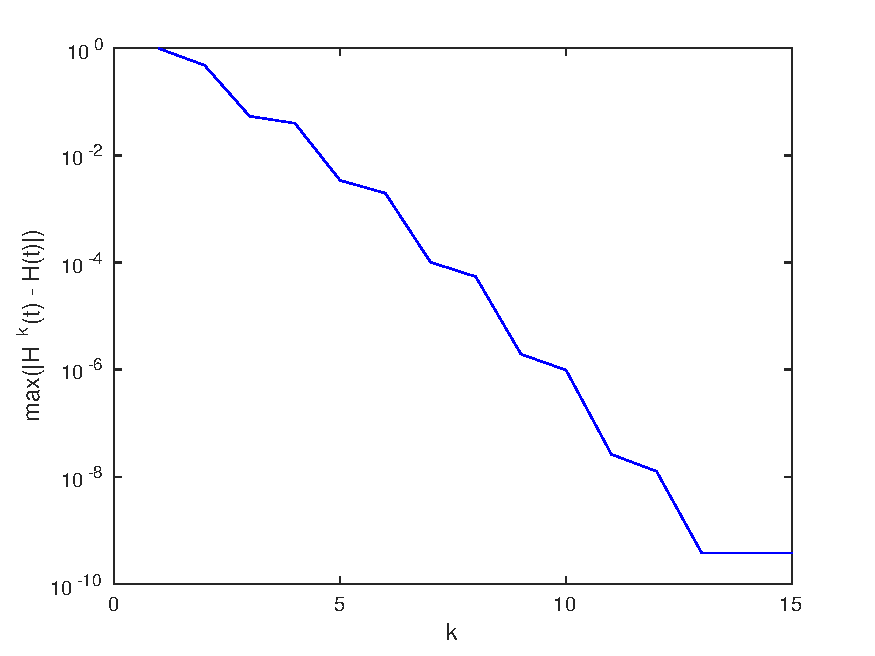
\includegraphics[width=0.45\textwidth]{03/Fig6-1.pdf}
  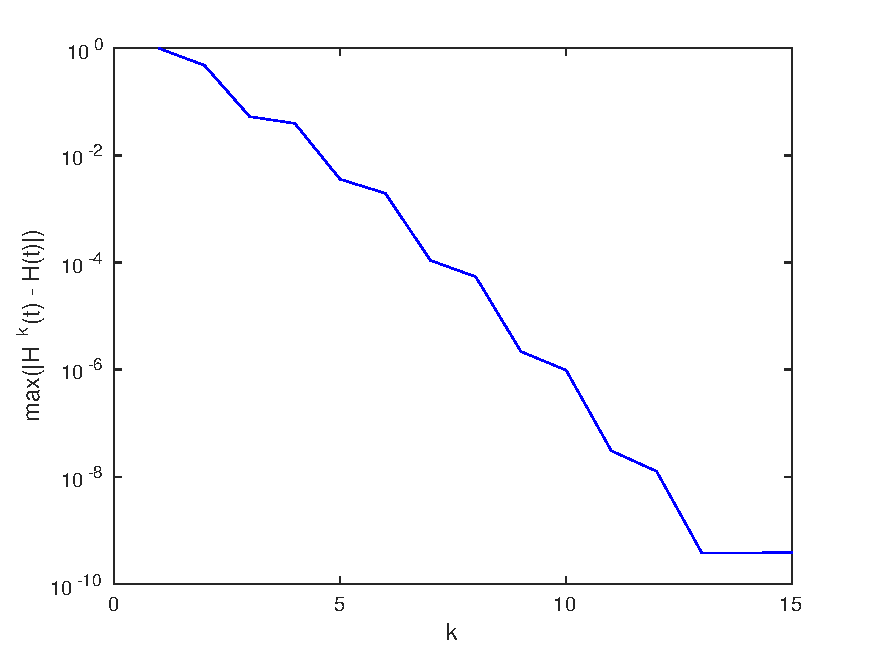
\includegraphics[width=0.45\textwidth]{03/Fig6-2.pdf}
  \caption{sin-Gordon 方程 \eqref{eq:singordon} 辛欧拉波形松弛方法(左图)和辛 Runge-Kutta 波形松弛方法(右图)在有窗口的情形下的比较}
  \label{fig:ex1winerr}
\end{figure}

\subsection*{例 2}
考虑 Fermi-Pasta-Ulam 问题 \cite{hairer2006geometric}. 其哈密尔顿函数为
\begin{equation*}
  \begin{aligned}
    H(q,p) &= \displaystyle{\frac{1}{2}} \sum_{i=1}^{2m} p_i +
    \displaystyle{\frac{\omega^2}{2}} \sum_{i=1}^{m} q_{m+i}^2 +
    \displaystyle{\frac{1}{4}}  \{ (x_1 - x_{m+1})^4 \\
    & \qquad + \sum_{i=1}^{m-1} (x_{i+1} - x_{m+i-1} - x_i - x_{m+i})^4 + (x_{m}
    - x_{2m})^4\},
  \end{aligned}
\end{equation*}
式中 $0<t\leq t_{\text{end}}$, $q_i~(i=1,2,\ldots,m)$ 为第 $i$ 个弹簧的位移,$q_{m+i}~(i=1,2,\ldots,m)$ 为第 $i$ 个弹簧拉伸或收缩的长度, $p_i~(i=1,2,\ldots,m)$ 是它们的速度,见图示~\ref{fig:fpu}.

\begin{figure}[h!]
  \centering
  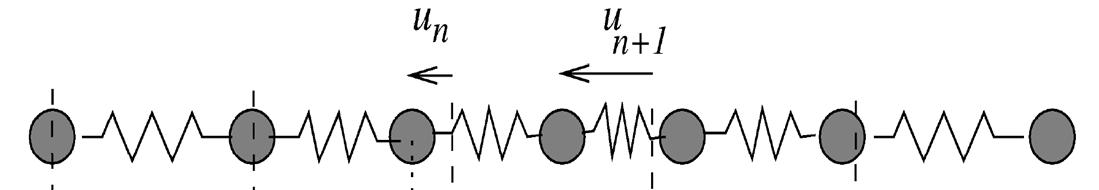
\includegraphics[width=0.7\textwidth]{03/FPUchainedependules.jpg}
  \caption{Fermi-Pasta-Ulam 示意图,图中两端固定}
  \label{fig:fpu}
\end{figure}

在本例中 \cite{hairer2006geometric}, 取 $m=3$, $\omega = 50$,
\begin{equation*}
  q_1(0) = 1, \quad p_1(0) = 1, \quad q_4(0) = \frac{1}{\omega}, \quad p_4(0) = 1,
\end{equation*}
并且其他的初值为 $0$.

首先考虑辛欧拉波形松弛方法~\eqref{eq:schemejacobi}. 取 $t_{\text{end}} = 10$, 步长为 $h = 10^{-3}$, 波形松弛迭代次数为 $k=20$. 对于窗口加速方法,取每个时间窗口为 $0.1$. 图 \ref{fig:ex2seucom} 展示了辛欧拉波形松弛方法无窗口加速(左图)和有窗口加速(右图)的比较.发现经典的波形松弛方法需要更多的步数才能收敛.全局最大误差为 $0.0195$.

\begin{figure}[h!]
  \centering
  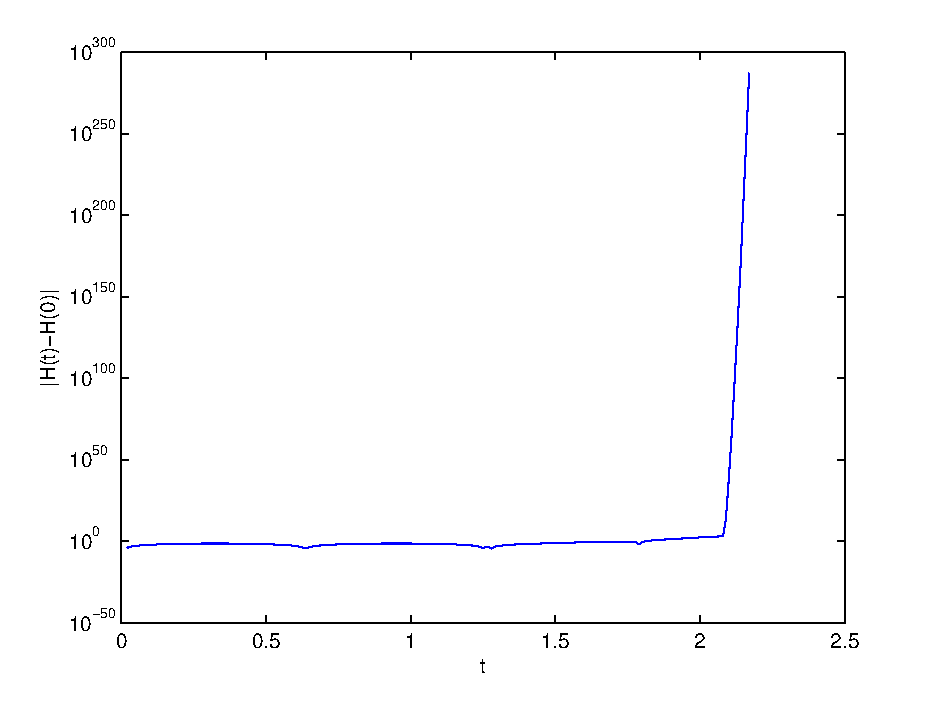
\includegraphics[width=0.45\textwidth]{03/Fig7-1.pdf}
  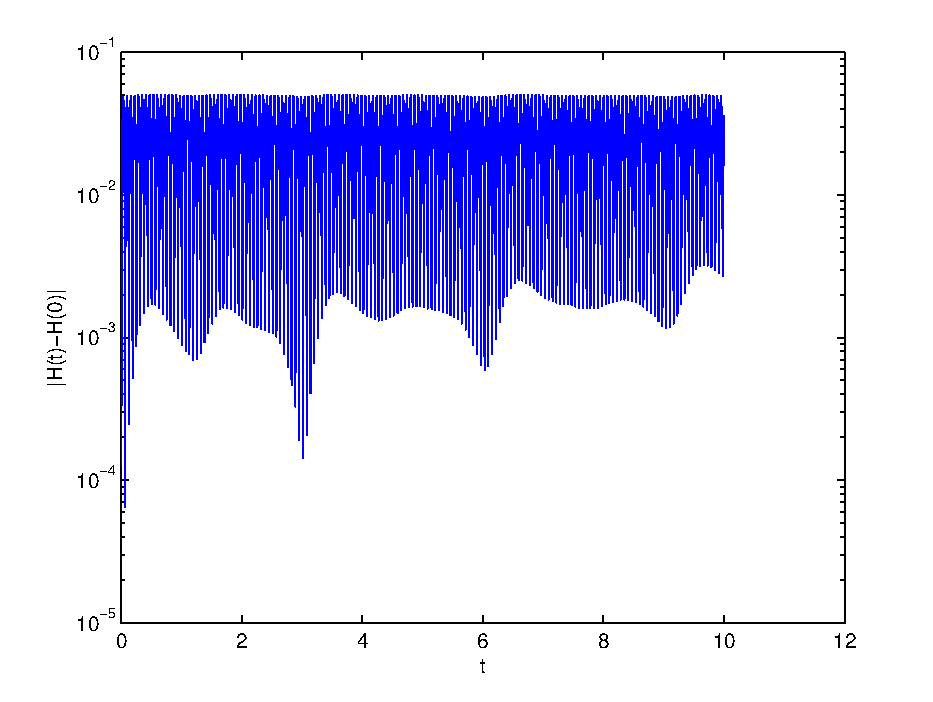
\includegraphics[width=0.45\textwidth]{03/Fig7-2.pdf}
  \caption{Fermi-Pasta-Ulam 问题辛欧拉波形松弛方法无窗口加速(左图)和有窗口加速(右图)的比较}
  \label{fig:ex2seucom}
\end{figure}

其次,考虑辛 Runge-Kutta 波形松弛方法~\eqref{eq:schemerkjacobi}. 取 $t_{\text{end}} = 10$, 步长为 $h = 1/100$, 波形松弛迭代次数为 $k=30$. 对于窗口加速方法,取每个时间窗口为 $0.1$. 图 \ref{fig:ex2srkcom} 展示了辛 Runge-Kutta 波形松弛方法无窗口加速(左图)和有窗口加速(右图)的比较.发现经典的波形松弛方法需要更多的步数才能收敛.在本例中使用了表 \ref{tbl:rk} 中的 Butcher 表,其中 $a = 1.351207$. 全局最大误差为 $1.0948e-06$.

\begin{figure}[h!]
  \centering
  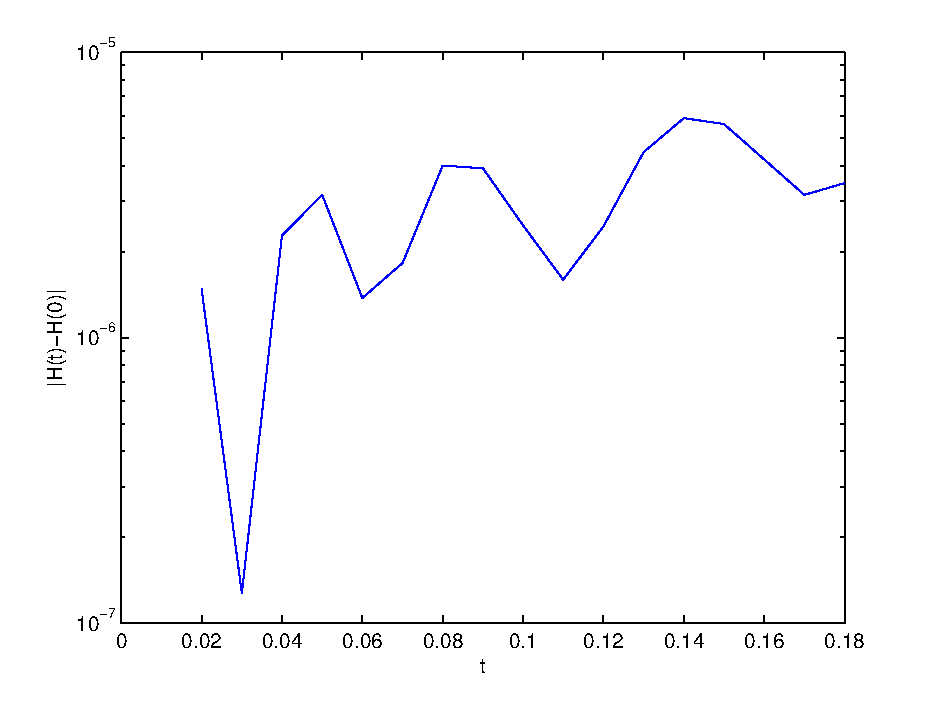
\includegraphics[width=0.45\textwidth]{03/Fig8-1.pdf}
  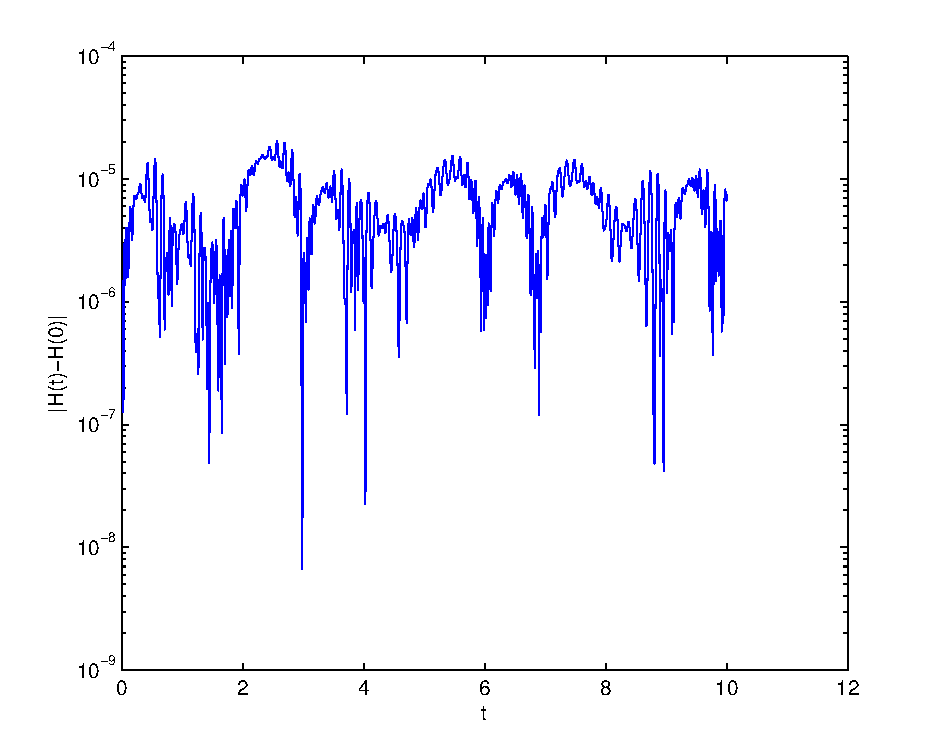
\includegraphics[width=0.45\textwidth]{03/Fig8-2.pdf}
  \caption{Fermi-Pasta-Ulam 问题辛 Runge-Kutta 波形松弛方法无窗口加速(左图)和有窗口加速(右图)的比较}
  \label{fig:ex2srkcom}
\end{figure}

\subsection*{例 3}
考虑如下的非线性波动方程 \cite{wu2013struc}
\begin{equation}\label{eq:nonlinwave}
  \left \{ \begin{array}{l}
      \displaystyle \frac{\partial^2 u }{\partial t^2}
      - \frac{\partial^2 u}{\partial x^2}
      = -\frac{1}{5} u^3 - \frac{1}{10} u^2, \quad 0<x<1, \; 0<t \leq t_{\text{end}},\\
      u(0,t) = u(1,t) = 0, \; u(x, 0) = \dfrac{\sin(\pi x)}{2}, \; u_t (x, 0) = 0.
    \end{array} \right.
\end{equation}
使用二阶中心差分方法,取空间步长为 $\Delta x = 1/N$ 和 $x_i = i \Delta x$, 得到如下的系统

\begin{equation*}
  \left \{ \begin{array}{l}
      \displaystyle \frac{d^2 U }{d t^2} + MU =F(t, U), \quad 0<t \leq t_{\text{end}},\\
      U(0) = (\dfrac{\sin(\pi x_1)}{2}, \ldots, \dfrac{\sin(\pi x_{N-1})}{2})^{T}, \quad U^{'} ={\bf 0},
    \end{array} \right.
\end{equation*}
式中 $U(t)=(u_1(t), \ldots. u_{N-1}(t))^{T}$ 和 $u_i(t) \approx u(x_i,t)$,
$x=1,2,\ldots,N-1$, 和
\begin{equation*}
  M = \frac{1}{\Delta x^2}
  \begin{pmatrix}
    2 & -1 & & &\\
    -1 & 2 & -1 & & \\
    & \ddots & \ddots& \ddots & \\
    & &-1 & 2 &-1 \\
    & & & -1&2\\
  \end{pmatrix},
\end{equation*}
\begin{equation*}
  F(t,U) = \left( -\frac{1}{5}u_1^3 -\frac{1}{10}u_1^2, \ldots,
    -\frac{1}{5}u_{N-1}^3 -\frac{1}{10}u_{N-1}^2 \right)^{T}.
\end{equation*}

令 $q := (q_1, \ldots, q_{N-1})^{T}= U$ 和 $p :=(p_1, \ldots, p_{N-1})^{T}:= \dot{q} = U^{'}$, 得到如下的哈密尔顿系统

\begin{equation}\label{eq:nonlinwaveH}
  \left \{ \begin{array}{l}
      \displaystyle \frac{d q }{d t} = p,\\
      \displaystyle \frac{d p }{d t} = -Mq - f(q),
    \end{array} \right.
\end{equation}
式中
\begin{equation*}
  f(q) = (\frac{1}{5} q_1^3 + \frac{1}{10} q_1^2, \ldots,
  \frac{1}{5} q_{N-1}^3 + \frac{1}{10} q_{N-1}^2)^{T},
\end{equation*}
初值条件为 $q(0)=(\frac{\sin(\pi x_1)}{2}, \ldots,
\frac{\sin(\pi x_{N-1})}{2})^{T}$, $p(0)={\bf 0}$, 其哈密尔顿函数为
$H(q,p) = \frac{1}{2}p^{ T}p + \frac{1}{2}q^{T}q + G(q)$, 式中
\begin{equation*}
  G(q) = \frac{1}{20} q_1^4 + \frac{1}{30} q_1^3 + \ldots + \frac{1}{20}
  q_{N-1}^4 + \frac{1}{30} q_{N-1}^3.
\end{equation*}

首先考虑辛欧拉波形松弛方法~\eqref{eq:schemejacobi}. 取 $t_{\text{end}} = 10$, $N=20$, 步长为 $h = 10^{-3}$, 波形松弛迭代次数为 $k=10$. 对于窗口加速方法,取每个时间窗口为 $0.1$. 图 \ref{fig:ex3seucom} 展示了辛欧拉波形松弛方法无窗口加速(左图)和有窗口加速(右图)的比较.发现经典的波形松弛方法需要更多的步数才能收敛.全局最大误差为 $0.0506$.

\begin{figure}[h!]
  \centering
  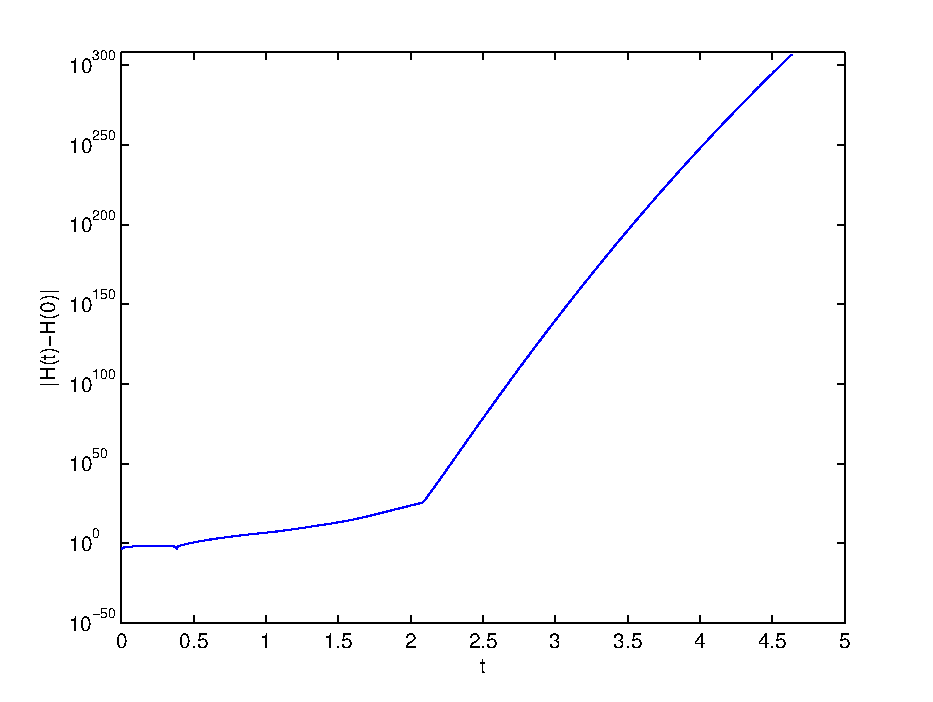
\includegraphics[width=0.45\textwidth]{03/Fig9-1.pdf}
  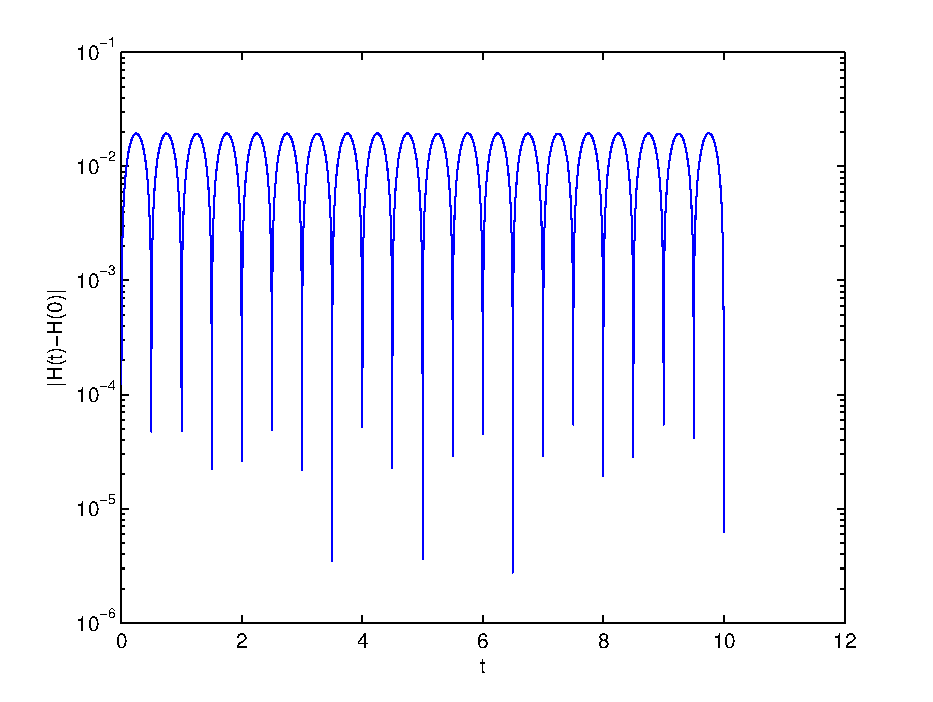
\includegraphics[width=0.45\textwidth]{03/Fig9-2.pdf}
  \caption{非线性波动方程 \eqref{eq:nonlinwave} 辛欧拉波形松弛方法无窗口加速(左图)和有窗口加速(右图)的比较}
  \label{fig:ex3seucom}
\end{figure}

其次,考虑辛 Runge-Kutta 波形松弛方法~\eqref{eq:schemerkjacobi}. 取 $t_{\text{end}} = 10$, $N=20$, 步长为 $h = 1/100$, 波形松弛迭代次数为 $k=30$. 对于窗口加速方法,取每个时间窗口为 $0.1$. 图 \ref{fig:ex3srkcom} 展示了辛 Runge-Kutta 波形松弛方法无窗口加速(左图)和有窗口加速(右图)的比较.发现经典的波形松弛方法需要更多的步数才能收敛.在本例中使用了表 \ref{tbl:rk} 中的 Butcher 表,其中 $a = 1.351207$. 全局最大误差为 $3.7003e-05$.

\begin{figure}[h!]
  \centering
  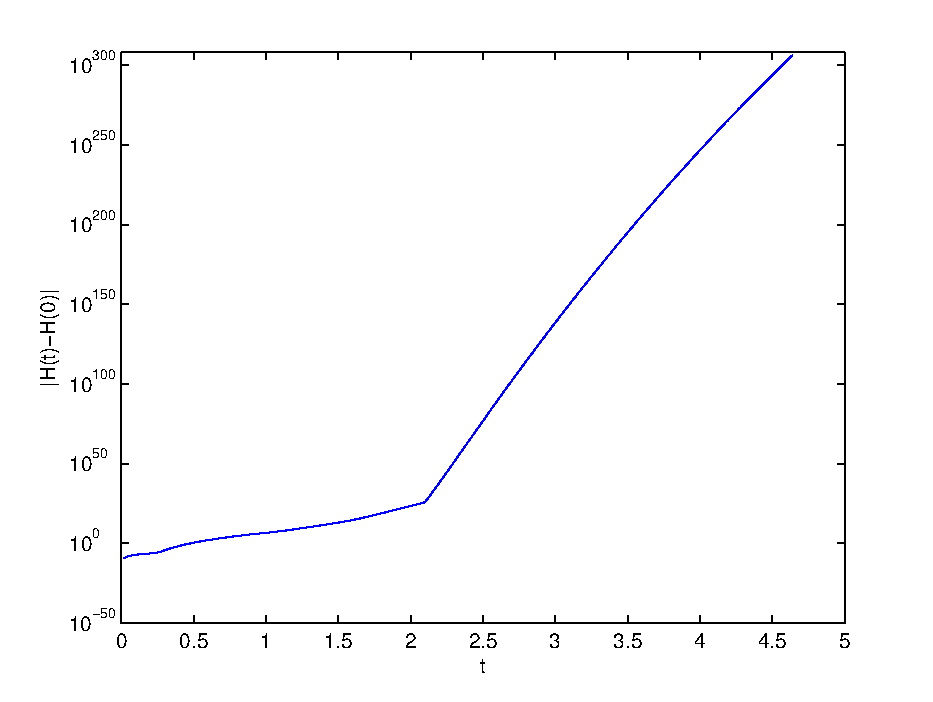
\includegraphics[width=0.45\textwidth]{03/Fig10-1.pdf}
  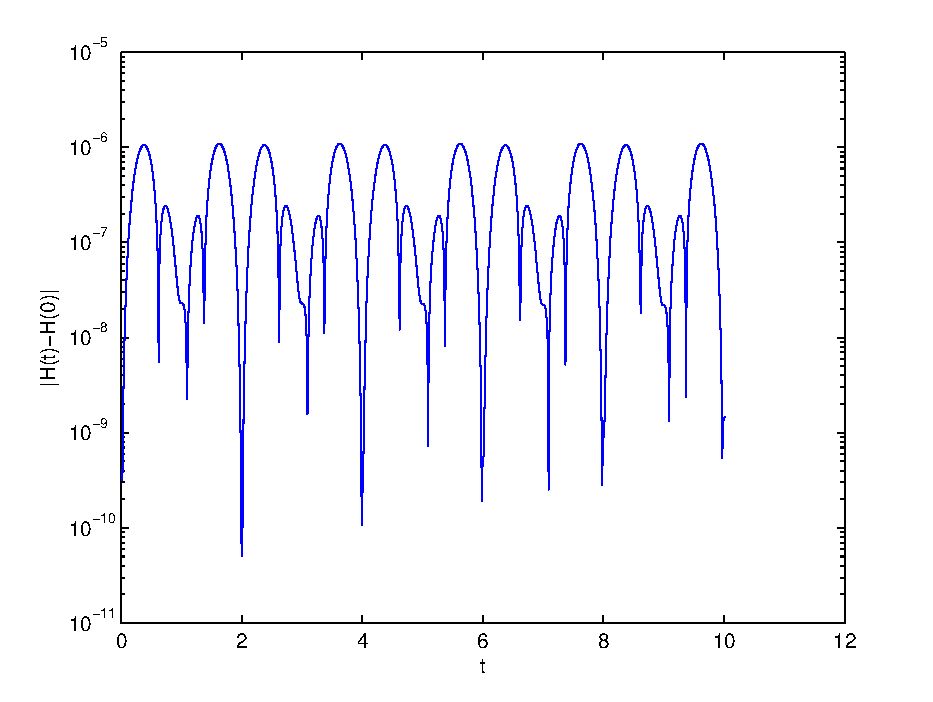
\includegraphics[width=0.45\textwidth]{03/Fig10-2.pdf}
  \caption{非线性波动方程 \eqref{eq:nonlinwave} 辛 Runge-Kutta 波形松弛方法无窗口加速(左图)和有窗口加速(右图)的比较}
  \label{fig:ex3srkcom}
\end{figure}

其数值解的示意图如图 \ref{fig:wavefig}.

\begin{figure}[h!]
  \centering
  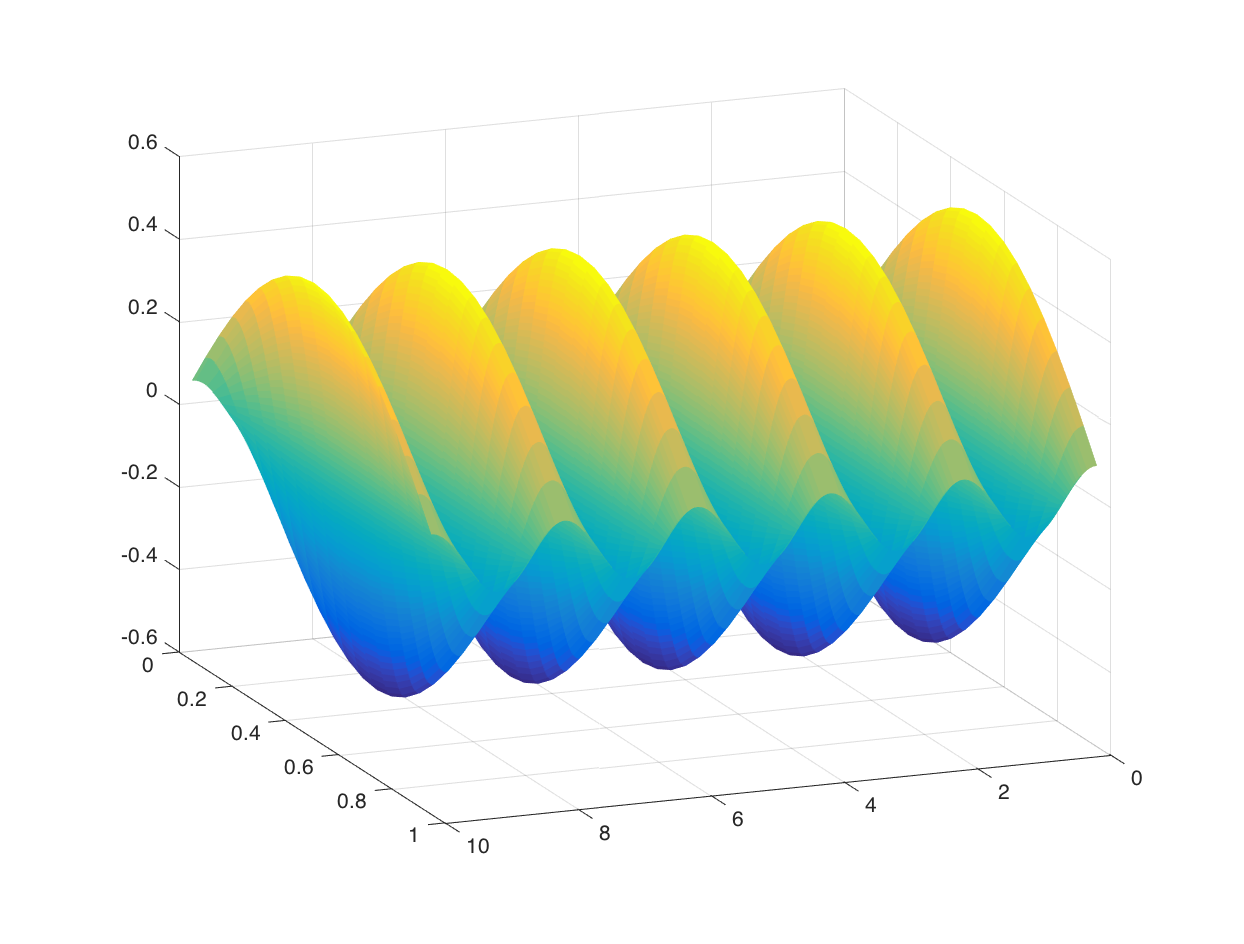
\includegraphics[width=0.7\textwidth]{03/wave.pdf}
  \caption{非线性波动方程的解示意图}
  \label{fig:wavefig}
\end{figure}

\subsection*{例 4}
最后给出一个计算的李群方程的例子,这个例子基于如下形式的三阶常微分方程

\begin{equation*}
  	\begin{pmatrix}
  		\dot{y_1}\\ \dot{y_2}\\ \dot{y_3}
  	\end{pmatrix}=
  	\begin{pmatrix}
  		0&y_3/I_3&-y_2/I_2\\
  		-y_3/I_3&0&y_1/I_1\\
  		y_2/I_2&-y_1/I_1&0
  	\end{pmatrix}
  	\begin{pmatrix}
  	y_1\\ y_2\\ y_3
  	\end{pmatrix},
 \end{equation*}
式中 $I_1,~I_2,~I_3$ 为常数.或者等价地写成
\begin{equation*}
  	\begin{aligned}
  		\dot{y_1}&=a_1 y_2 y_3,\qquad a_1=(I_2-I_3)/(I_2I_3),\\
  		\dot{y_2}&=a_2 y_3 y_1,\qquad a_3=(I_3-I_1)/(I_3I_1),\\
  		\dot{y_3}&=a_3 y_1 y_2,\qquad a_3=(I_1-I_2)/(I_1I_2).
  	\end{aligned}
\end{equation*}
根据李群方程的形式,可以知道
\begin{equation*}
  	A(t,Y)=
  	\begin{pmatrix}
  		0&y_3/I_3&-y_2/I_2\\
  		-y_3/I_3&0&y_1/I_1\\
  		y_2/I_2&-y_1/I_1&0
  	\end{pmatrix}.
 \end{equation*}

该问题描述了刚体的自由运动,其质心在中点.该系统有两个守恒量,可以通过如下计算得到.首先根据如下的式子
\begin{equation*}
	a_1+a_2+a_3=(\frac{1}{I_3}-\frac{1}{I_2})+(\frac{1}{I_1}-\frac{1}{I_3})+(\frac{1}{I_2}-\frac{1}{I_1})=0,
\end{equation*}
得到守恒量
\begin{equation*}
	{y_1}^2+{y_2}^2+{y_3}^2.
\end{equation*}
再根据
\begin{equation*}
	\frac{a_1}{I_1}+\frac{a_2}{I_2}+\frac{a_3}{I_3}=\frac{(I_2-I_3)+(I_3-I_1)+(I_1-I_2)}{I_1I_2I_3}=0,
\end{equation*}
可以得到守恒量
\begin{equation*}
	H(y_1,y_2,y_3)=\frac{1}{2}(\frac{{y_1}^2}{I_1}+\frac{{y_2}^2}{I_2}+\frac{{y_3}^2}{I_3}).
\end{equation*}

可以看到,第一个守恒量描述刚体的形状不变,第二个则描述动能守恒.该问题的解可以看作是一个球体和一个椭球的交线,因此,该解在一个稳定的椭圆上.

这里,使用表 \ref{tbl:04rk3} 中的 Butcher 表,该表对应的 Runge-Kutta 法是一个辛方法.

\begin{table}[h!]
  \centering
  \caption{三阶 Butcher 表}
  \label{tbl:04rk3}
  \begin{tabular}{c|ccc}
    $\frac{1}{2}a$ & $\frac{1}{2}a$ & & \\
    $\frac{3}{2}a$ & $a$ &$\frac{1}{2}a$  & \\
    $\frac{1}{2} + a$ & $a$ & $a$ &$\frac{1}{2}-a$\\
    \hline
    & $a$ &$a$ & $1-2a$\\
  \end{tabular}
\end{table}
其中$a = 1.351207$.

通过计算,能得到如下的数值结果,如图 \ref{fig:rkmk3}. 可以看出,该方法能够保持原格式应有的效果,得到了一个保结构的数值算法.这里,取步长为 $0.3$, 共取了 $500$ 步,分 $10$ 个窗口计算.

\begin{figure}[h!]
  \centering
  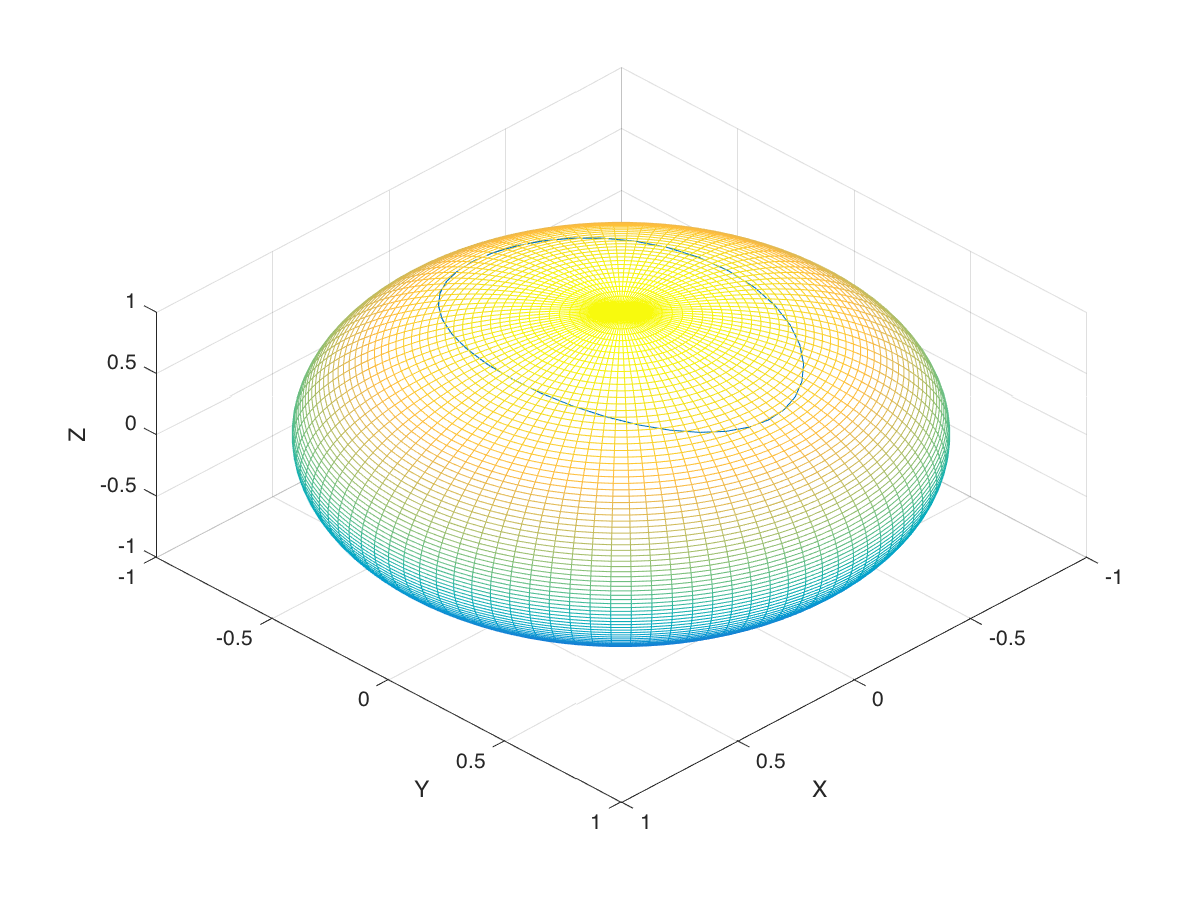
\includegraphics[width=0.7\textwidth]{03/rkmk3.png}
  \caption{改进后方法的数值结果}
  \label{fig:rkmk3}
\end{figure}

 \section{小结}\label{sec:03conclusion}
 \esection{Brief Summary}
在本章中,我们首先提出了求解哈密尔顿系统的辛波形松弛方法.该方法指明了针对该系统应该如何选择分裂函数的问题.为了加速算法,使用了窗口加速技术.我们从连续系统和离散系统两个方面给出了系统哈密尔顿量在迭代下收敛到守恒的量的性质,并在数值结果中验证了这一点.我们还给出了算法的基本流程.

其次,在此基础上,我们对李群方法做出了详细地介绍,分析了其优点和不足,并对隐式的 RK-MK 方法提出了一种改进方法,即用波形松弛方法进行修正.该方法能够缓解隐式 RK-MK 方法的复杂性计算问题,把隐式的计算化为较为简单的显式或者半隐式问题,并用窗口技术进行加速.

最后,我们通过数值结果能够说明该方法的有效性.


\chapter{结论与展望}
\echapter{Conclusions and Expectations}
在本章, 将总结前面章节的主要内容, 并为下一步的研究工作进行展望.
\section{结论}
\esection{Conclusions}
本博士论文主要围绕辛方法,波形松弛方法和李群方法进行了一些数值方法和解析方法的研究.
通过对不守恒的系统进行变换得到了形式较好的守恒系统.通过对隐式格式的修正得到了较为
容易的显式格式.通过李点对称变换得到了形式较为简单的约化方程.具体内容包括以下几个方面:

(一) 在第~2~章,提出了一种新的求解带有齐次边界条件的电报方程的方法.该方法有效
利用了一个将非哈密尔顿系统化为哈密尔顿系统的变换,结合了辛方法的特性,得到了
较好的效果.本章中,讨论了该算法的阶条件、CFL 条件、长时间性质和局限性.在空间离散上
取了二阶的离散格式,得到了 $O(\Delta x^2+ \Delta t^k)$ 的误差界. 该方法的一个优点是
利用了辛方法长时间求解的好的性质.另外,我们的解可以看作一个很优美的哈密尔顿系统
乘以一个函数的结果.方法的基本思想是先变换,再求解,再逆变换,和傅立叶变换的思想
比较类似.数值结果展示了阶条件,算法的有效性和长时间性质.该方法不局限于使用文中提及
的辛格式,其他合适的辛格式也可以使用进来.非齐次的问题,需要增加两个分量来求解,该部分
在文中注解部分有所提及.

(二) 在第~3~章, 将复合变分准则应用到了 (2+1) 维拓展 QZK 方程.应用这些李点对称,
证明了 (2+1) 维拓展 QZK 方程是自共轭的,并且构造了其守恒律.接着,给出了一维子代数
最优系统.通过相应的相似不变量的相似变换, (2+1) 维拓展 QZK 方程变为线性的偏微分方程.
说明了李点对称方法对于拓展 QZK 方程是有效的,该结果对研究该方程起到了积极的指导作用.

(三) 在第~4~章,对波形松弛方法和辛方法做了介绍,并将其应用到哈密尔顿系统上,
提出了求解哈密尔顿系统的辛波形松弛方法,得到了一个很好的设计该格式的等式.该方法
结合了辛方法和波形松弛方法双方的优势,解决了求解隐式辛格式的困难,同时指明了针对该
系统应该如何选择分裂函数的问题.使用窗口加速技术来加速该方法.在辛波形松弛方法的
基础上,对李群方法做出了详细地介绍,分析了其优点和不足,分析了隐式 RK-MK 方法的
必要性,并基于辛波形松弛方法的思路,对隐式的 RK-MK 方法提出了一种改进方法,即用波形
松弛方法进行修正.该方法能够缓解隐式 RK-MK 方法的复杂性计算问题,把隐式的计算化为
较为简单的显式或者半隐式问题,并再次使用窗口计算进行加速.从连续问题和离散后问题
分别给出了系统哈密尔顿量在迭代下收敛到守恒的量的性质,并给出了一个改进的李群 RK-MK
算法,还给出了算法的基本流程.在给出的数值结果中,能看到较好的对辛结构和李群
结构的保持,从而说明了该类方法的可行性和有效性.

\section{展望}
\esection{Expectations}
在本博士论文的基础上,可以从如下几个方面进行进一步的深入研究.一是基于 RK-MK
方法,建立在流形上的保结构数值格式,这将给隐式 RK-MK 方法的使用提供理论依据.二是对
波形松弛方法进行修正和改进,使得数值结果收敛到相应数值格式这一问题变为提高数值格式
的精度.三是对辛波形松弛方法设计并行算法,使波形松弛可以用来设计并行算法的事实成为可能.


\xjtuendcontent

\xjtuspchapter{致\quad 谢}{致\quad 谢}{Acknowledgements}

人生路漫漫,不觉间来交大已经十个春秋.在这段短暂又漫长的人生路里,是这所百年名校教诲培养着我,指引我前进.

我在这里首先要感谢我的导师蒋耀林教授,我成长的每一步和他是分不开的.是老师教导我如何正确选择人生道路,让我少走些弯路;
是老师纠正我性格中的每一个缺点,让我变得越来越坚强强大;是老师教给我``追求=坚持''的等式,让我驶向前方的道路是意志坚定;
是老师给了我一个相对自由的学习空间,让我这些年不受世俗所累安心学习.蒋老师付出的每一分汗水,每一次教诲我都铭记在心,
并以此作为指引我走好前方的路.

我还要感谢在交大教过我的每一位老师,特别是数学分析课程的李惜雯老师,使我领略到了数学的严谨;拓扑学课上的李洪军老师,
将枯燥的课程讲得那样有趣;我重修体育课的张军老师,给我很大的帮助.

我要感谢我的父母,爷爷奶奶及家人,辛辛苦苦把我培养大,不辞辛苦,任劳任怨,对我无私地投入与教导,才有了现在的我.

我要感谢我认识的和认识我的每一个人,他们带我了解了不同的世界,我也从他们那里学到了不少知识.其中包括TUNA组织和里面的朋友们,
xiaq(肖骐),大鹰(汪彧之),康哥(王康)等;我很佩服的姬神(孔祥杰);我很好的朋友们,郑捷宇,张戈,钱黎黎等;打网球的朋友们,
高婷,张晓荷,唐杏,吴杰等;以及认识的大神冯雪,董老师董梦馨,张康,朱婕等等.

我还要感谢同师门的师兄弟姐妹们,是他们让我变得强大,羽翼丰满.他们是张辉,李立,高宁,陈芳,孔旭,刘军,王晓龙,陈海宝,黄芬芬,李荣建,
宋博,刘亚婧,杨媚,彭国俊,丁小丽,许微微,贾纪腾,肖志华,祁振中,袁嘉薇,梁猛,王彦斐,陈诚,杨云波,孙希超,邓定文,邱志勇,杨钧满,苗真,张伟等.
还有工作了的师兄师姐李辉,高静,康艳梅,王宇莹等.

路漫漫其修远兮,吾将上下而求索.愿我在今后的人生道路上,带着积累多年的知识与本领,继续辉煌地走好每一步.


% 将你要引用的文献的 BibTeX 放入 bibliography.bib \xjtubib{reference/phdthesis}

% 将你要引用的文献的 BibTeX 放入 bibliography.bib \xjtubib{reference/mythesis}
% from Hui其中chinesebst是我自己生成的参考文献风格,比较符合中国人的习惯参考文
% 献plain,unsrt,alpha,abbrev,chinesebst,GBT7714-2005NLang,GBT7714-2005AYLang

%\phantomsection \addcontentsline{toc}{chapter}{参考文献}
%\addcontentsline{toe}{chapter}{References} \fontsize{10.5pt}{10.5pt}\selectfont
%\setlength{\baselineskip}{15pt} \addtolength{\bibsep}{-2mm}
%\bibliographystyle{setup/chinesebst1} 
%\bibliography{reference/phdthesis}

\xjtubib{reference/phdthesis}

% \xjtuappendix

% \input{body/appendice.tex}

% \xjtuendappendix

\xjtuspchapter{攻读博士期间取得的研究成果}{攻读博士期间取得的研究成
  果}{Achievements}

% 已发表或已录用的学术论文、已出版的专著/译著、已获授权的专利按参考文献格式列出。
% 科研获奖,列出格式为:获奖人(排名情况).项目名称.奖项名称及等级,发奖机构,
% 获奖时间.与学位论文相关的其它成果参照参考文献格式列出。全部研究成果连续编号编
% 排。

\renewcommand\labelenumi{[\theenumi]}
{\xiaosi \noindent 一、已发表或已录用的学术论文 \begin{enumerate}
  \begin{spacing}{1.0}
  \item Y. Lu and Y. L. Jiang. Symplectic schemes for telegraph equations[J]. Journal of Computational Mathematics, 2016, 34(3):326--340.~(国际知名~SCI~期刊)

  \item Y. L. Jiang, Y. Lu, and C. Chen. Conservation laws and optimal system of extended quantum Zakharov-Kuznetsov equation[J]. Journal of Nonlinear Mathematical Physics, 2016, 23(2): 157--166.~(国际知名~SCI~期刊, IDS~号: DQ2PO)

  \item Y. Lu, Y.L. Jiang and B. Song. Symplectic waveform relaxation methods for Hamiltonian systems[J]. Applied Mathematics and Computation, 2017, 292: 228--239.~(国际知名~SCI~期刊, IDS~号: DX5CM)
  \end{spacing}
\end{enumerate}

\vspace{12pt}

\noindent 二、科研项目
\begin{spacing}{1.0}
  \begin{enumerate}
  \item 大型并行计算的时空区域分解方法: 2011-2014, 国际科技合作项目(科技部), 参加
    者.
  \item 集成电路模拟中的数学方法研究: 2014-2017, 国家自然科学基金项目, 参加者.
  \end{enumerate}
\end{spacing}
}

% \xjtuacademicintegrity
\cleardoublepage
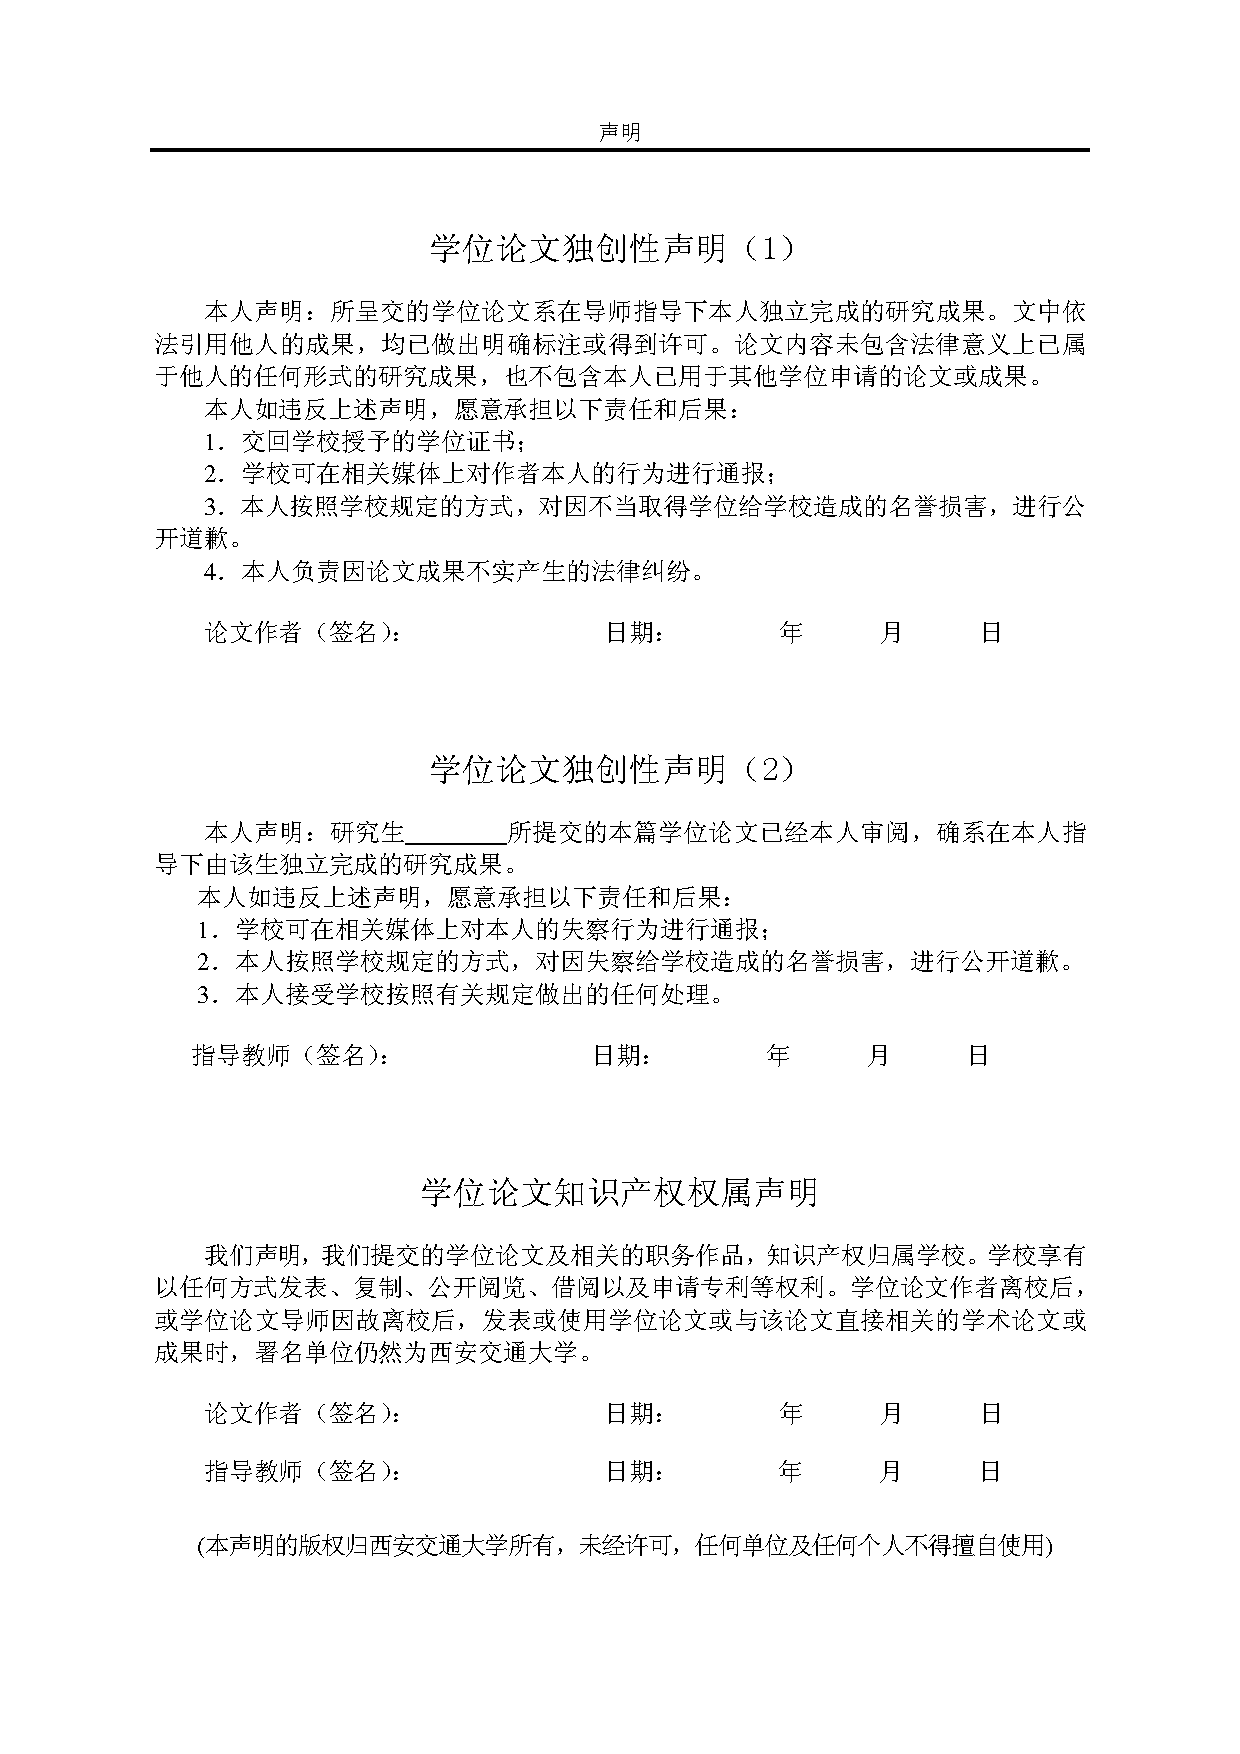
\includepdf[offset=0 18mm]{info/shengming.pdf}

\end{document}
